% Options for packages loaded elsewhere
\PassOptionsToPackage{unicode}{hyperref}
\PassOptionsToPackage{hyphens}{url}
\PassOptionsToPackage{dvipsnames,svgnames,x11names}{xcolor}
%
\documentclass[
  letterpaper,
  DIV=11,
  numbers=noendperiod]{scrreprt}

\usepackage{amsmath,amssymb}
\usepackage{iftex}
\ifPDFTeX
  \usepackage[T1]{fontenc}
  \usepackage[utf8]{inputenc}
  \usepackage{textcomp} % provide euro and other symbols
\else % if luatex or xetex
  \usepackage{unicode-math}
  \defaultfontfeatures{Scale=MatchLowercase}
  \defaultfontfeatures[\rmfamily]{Ligatures=TeX,Scale=1}
\fi
\usepackage{lmodern}
\ifPDFTeX\else  
    % xetex/luatex font selection
\fi
% Use upquote if available, for straight quotes in verbatim environments
\IfFileExists{upquote.sty}{\usepackage{upquote}}{}
\IfFileExists{microtype.sty}{% use microtype if available
  \usepackage[]{microtype}
  \UseMicrotypeSet[protrusion]{basicmath} % disable protrusion for tt fonts
}{}
\makeatletter
\@ifundefined{KOMAClassName}{% if non-KOMA class
  \IfFileExists{parskip.sty}{%
    \usepackage{parskip}
  }{% else
    \setlength{\parindent}{0pt}
    \setlength{\parskip}{6pt plus 2pt minus 1pt}}
}{% if KOMA class
  \KOMAoptions{parskip=half}}
\makeatother
\usepackage{xcolor}
\setlength{\emergencystretch}{3em} % prevent overfull lines
\setcounter{secnumdepth}{5}
% Make \paragraph and \subparagraph free-standing
\ifx\paragraph\undefined\else
  \let\oldparagraph\paragraph
  \renewcommand{\paragraph}[1]{\oldparagraph{#1}\mbox{}}
\fi
\ifx\subparagraph\undefined\else
  \let\oldsubparagraph\subparagraph
  \renewcommand{\subparagraph}[1]{\oldsubparagraph{#1}\mbox{}}
\fi

\usepackage{color}
\usepackage{fancyvrb}
\newcommand{\VerbBar}{|}
\newcommand{\VERB}{\Verb[commandchars=\\\{\}]}
\DefineVerbatimEnvironment{Highlighting}{Verbatim}{commandchars=\\\{\}}
% Add ',fontsize=\small' for more characters per line
\usepackage{framed}
\definecolor{shadecolor}{RGB}{241,243,245}
\newenvironment{Shaded}{\begin{snugshade}}{\end{snugshade}}
\newcommand{\AlertTok}[1]{\textcolor[rgb]{0.68,0.00,0.00}{#1}}
\newcommand{\AnnotationTok}[1]{\textcolor[rgb]{0.37,0.37,0.37}{#1}}
\newcommand{\AttributeTok}[1]{\textcolor[rgb]{0.40,0.45,0.13}{#1}}
\newcommand{\BaseNTok}[1]{\textcolor[rgb]{0.68,0.00,0.00}{#1}}
\newcommand{\BuiltInTok}[1]{\textcolor[rgb]{0.00,0.23,0.31}{#1}}
\newcommand{\CharTok}[1]{\textcolor[rgb]{0.13,0.47,0.30}{#1}}
\newcommand{\CommentTok}[1]{\textcolor[rgb]{0.37,0.37,0.37}{#1}}
\newcommand{\CommentVarTok}[1]{\textcolor[rgb]{0.37,0.37,0.37}{\textit{#1}}}
\newcommand{\ConstantTok}[1]{\textcolor[rgb]{0.56,0.35,0.01}{#1}}
\newcommand{\ControlFlowTok}[1]{\textcolor[rgb]{0.00,0.23,0.31}{#1}}
\newcommand{\DataTypeTok}[1]{\textcolor[rgb]{0.68,0.00,0.00}{#1}}
\newcommand{\DecValTok}[1]{\textcolor[rgb]{0.68,0.00,0.00}{#1}}
\newcommand{\DocumentationTok}[1]{\textcolor[rgb]{0.37,0.37,0.37}{\textit{#1}}}
\newcommand{\ErrorTok}[1]{\textcolor[rgb]{0.68,0.00,0.00}{#1}}
\newcommand{\ExtensionTok}[1]{\textcolor[rgb]{0.00,0.23,0.31}{#1}}
\newcommand{\FloatTok}[1]{\textcolor[rgb]{0.68,0.00,0.00}{#1}}
\newcommand{\FunctionTok}[1]{\textcolor[rgb]{0.28,0.35,0.67}{#1}}
\newcommand{\ImportTok}[1]{\textcolor[rgb]{0.00,0.46,0.62}{#1}}
\newcommand{\InformationTok}[1]{\textcolor[rgb]{0.37,0.37,0.37}{#1}}
\newcommand{\KeywordTok}[1]{\textcolor[rgb]{0.00,0.23,0.31}{#1}}
\newcommand{\NormalTok}[1]{\textcolor[rgb]{0.00,0.23,0.31}{#1}}
\newcommand{\OperatorTok}[1]{\textcolor[rgb]{0.37,0.37,0.37}{#1}}
\newcommand{\OtherTok}[1]{\textcolor[rgb]{0.00,0.23,0.31}{#1}}
\newcommand{\PreprocessorTok}[1]{\textcolor[rgb]{0.68,0.00,0.00}{#1}}
\newcommand{\RegionMarkerTok}[1]{\textcolor[rgb]{0.00,0.23,0.31}{#1}}
\newcommand{\SpecialCharTok}[1]{\textcolor[rgb]{0.37,0.37,0.37}{#1}}
\newcommand{\SpecialStringTok}[1]{\textcolor[rgb]{0.13,0.47,0.30}{#1}}
\newcommand{\StringTok}[1]{\textcolor[rgb]{0.13,0.47,0.30}{#1}}
\newcommand{\VariableTok}[1]{\textcolor[rgb]{0.07,0.07,0.07}{#1}}
\newcommand{\VerbatimStringTok}[1]{\textcolor[rgb]{0.13,0.47,0.30}{#1}}
\newcommand{\WarningTok}[1]{\textcolor[rgb]{0.37,0.37,0.37}{\textit{#1}}}

\providecommand{\tightlist}{%
  \setlength{\itemsep}{0pt}\setlength{\parskip}{0pt}}\usepackage{longtable,booktabs,array}
\usepackage{calc} % for calculating minipage widths
% Correct order of tables after \paragraph or \subparagraph
\usepackage{etoolbox}
\makeatletter
\patchcmd\longtable{\par}{\if@noskipsec\mbox{}\fi\par}{}{}
\makeatother
% Allow footnotes in longtable head/foot
\IfFileExists{footnotehyper.sty}{\usepackage{footnotehyper}}{\usepackage{footnote}}
\makesavenoteenv{longtable}
\usepackage{graphicx}
\makeatletter
\def\maxwidth{\ifdim\Gin@nat@width>\linewidth\linewidth\else\Gin@nat@width\fi}
\def\maxheight{\ifdim\Gin@nat@height>\textheight\textheight\else\Gin@nat@height\fi}
\makeatother
% Scale images if necessary, so that they will not overflow the page
% margins by default, and it is still possible to overwrite the defaults
% using explicit options in \includegraphics[width, height, ...]{}
\setkeys{Gin}{width=\maxwidth,height=\maxheight,keepaspectratio}
% Set default figure placement to htbp
\makeatletter
\def\fps@figure{htbp}
\makeatother
% definitions for citeproc citations
\NewDocumentCommand\citeproctext{}{}
\NewDocumentCommand\citeproc{mm}{%
  \begingroup\def\citeproctext{#2}\cite{#1}\endgroup}
\makeatletter
 % allow citations to break across lines
 \let\@cite@ofmt\@firstofone
 % avoid brackets around text for \cite:
 \def\@biblabel#1{}
 \def\@cite#1#2{{#1\if@tempswa , #2\fi}}
\makeatother
\newlength{\cslhangindent}
\setlength{\cslhangindent}{1.5em}
\newlength{\csllabelwidth}
\setlength{\csllabelwidth}{3em}
\newenvironment{CSLReferences}[2] % #1 hanging-indent, #2 entry-spacing
 {\begin{list}{}{%
  \setlength{\itemindent}{0pt}
  \setlength{\leftmargin}{0pt}
  \setlength{\parsep}{0pt}
  % turn on hanging indent if param 1 is 1
  \ifodd #1
   \setlength{\leftmargin}{\cslhangindent}
   \setlength{\itemindent}{-1\cslhangindent}
  \fi
  % set entry spacing
  \setlength{\itemsep}{#2\baselineskip}}}
 {\end{list}}
\usepackage{calc}
\newcommand{\CSLBlock}[1]{\hfill\break\parbox[t]{\linewidth}{\strut\ignorespaces#1\strut}}
\newcommand{\CSLLeftMargin}[1]{\parbox[t]{\csllabelwidth}{\strut#1\strut}}
\newcommand{\CSLRightInline}[1]{\parbox[t]{\linewidth - \csllabelwidth}{\strut#1\strut}}
\newcommand{\CSLIndent}[1]{\hspace{\cslhangindent}#1}

\KOMAoption{captions}{tableheading}
\makeatletter
\@ifpackageloaded{tcolorbox}{}{\usepackage[skins,breakable]{tcolorbox}}
\@ifpackageloaded{fontawesome5}{}{\usepackage{fontawesome5}}
\definecolor{quarto-callout-color}{HTML}{909090}
\definecolor{quarto-callout-note-color}{HTML}{0758E5}
\definecolor{quarto-callout-important-color}{HTML}{CC1914}
\definecolor{quarto-callout-warning-color}{HTML}{EB9113}
\definecolor{quarto-callout-tip-color}{HTML}{00A047}
\definecolor{quarto-callout-caution-color}{HTML}{FC5300}
\definecolor{quarto-callout-color-frame}{HTML}{acacac}
\definecolor{quarto-callout-note-color-frame}{HTML}{4582ec}
\definecolor{quarto-callout-important-color-frame}{HTML}{d9534f}
\definecolor{quarto-callout-warning-color-frame}{HTML}{f0ad4e}
\definecolor{quarto-callout-tip-color-frame}{HTML}{02b875}
\definecolor{quarto-callout-caution-color-frame}{HTML}{fd7e14}
\makeatother
\makeatletter
\@ifpackageloaded{bookmark}{}{\usepackage{bookmark}}
\makeatother
\makeatletter
\@ifpackageloaded{caption}{}{\usepackage{caption}}
\AtBeginDocument{%
\ifdefined\contentsname
  \renewcommand*\contentsname{Table of contents}
\else
  \newcommand\contentsname{Table of contents}
\fi
\ifdefined\listfigurename
  \renewcommand*\listfigurename{List of Figures}
\else
  \newcommand\listfigurename{List of Figures}
\fi
\ifdefined\listtablename
  \renewcommand*\listtablename{List of Tables}
\else
  \newcommand\listtablename{List of Tables}
\fi
\ifdefined\figurename
  \renewcommand*\figurename{Figure}
\else
  \newcommand\figurename{Figure}
\fi
\ifdefined\tablename
  \renewcommand*\tablename{Table}
\else
  \newcommand\tablename{Table}
\fi
}
\@ifpackageloaded{float}{}{\usepackage{float}}
\floatstyle{ruled}
\@ifundefined{c@chapter}{\newfloat{codelisting}{h}{lop}}{\newfloat{codelisting}{h}{lop}[chapter]}
\floatname{codelisting}{Listing}
\newcommand*\listoflistings{\listof{codelisting}{List of Listings}}
\makeatother
\makeatletter
\makeatother
\makeatletter
\@ifpackageloaded{caption}{}{\usepackage{caption}}
\@ifpackageloaded{subcaption}{}{\usepackage{subcaption}}
\makeatother
\ifLuaTeX
  \usepackage{selnolig}  % disable illegal ligatures
\fi
\usepackage{bookmark}

\IfFileExists{xurl.sty}{\usepackage{xurl}}{} % add URL line breaks if available
\urlstyle{same} % disable monospaced font for URLs
\hypersetup{
  pdftitle={Multilevel Multilingual},
  pdfauthor={Andrew Grogan-Kaylor},
  colorlinks=true,
  linkcolor={blue},
  filecolor={Maroon},
  citecolor={Blue},
  urlcolor={Blue},
  pdfcreator={LaTeX via pandoc}}

\title{Multilevel Multilingual}
\usepackage{etoolbox}
\makeatletter
\providecommand{\subtitle}[1]{% add subtitle to \maketitle
  \apptocmd{\@title}{\par {\large #1 \par}}{}{}
}
\makeatother
\subtitle{Multilevel Models in Stata, R and Julia}
\author{Andrew Grogan-Kaylor}
\date{2024-09-19}

\begin{document}
\maketitle

\renewcommand*\contentsname{Table of contents}
{
\hypersetup{linkcolor=}
\setcounter{tocdepth}{2}
\tableofcontents
}
\listoftables
\bookmarksetup{startatroot}

\chapter{Multilevel Multilingual}\label{multilevel-multilingual}

\begin{quote}
``This curious world which we inhabit is more wonderful than it is
convenient\ldots{}'' (Thoreau, 1975)
\end{quote}

\begin{quote}
``Mathematics is my secret. My secret weakness. I feel like a stubborn,
helpless fool in the middle of a problem. Trapped and crazed. Also,
thrilled.'' (Schanen, 2021)
\end{quote}

\section{Introduction}\label{introduction}

Below, I describe the use of \href{https://www.stata.com/}{Stata}
(StataCorp, 2023), \href{https://www.r-project.org/}{R} (Bates et al.,
2015; R Core Team, 2023), and \href{https://www.julialang.org/}{Julia}
(Bates, 2024; Bezanson et al., 2017) to estimate multilevel models.

All of these software packages can estimate multilevel models and can
visualize relationships in the data. However, there are substantial
differences between the different packages: Stata is proprietary
\emph{for cost} software, which is very well documented and very
intuitive. While it costs money to purchase Stata, the price is often
very reasonable for academic and educational use. R is \emph{free} open
source software which is less intuitive, but there are many excellent
resources for learning R. There is often a cost associated with
purchasing books and other materials for learning R, which sometimes
feels like it offsets the fact that R is free. Julia is newer open
source software, also \emph{free}, and ostensibly much faster than
either Stata or R, which may be an important advantage when running
multilevel models with very large data sets. At this point in time, both
Stata and R feel much more \emph{stable} than Julia which is still
evolving software.

While any of these software packages can be used for learning and
estimating multilevel models, I will offer my own opinion--based upon 15
years of teaching multilevel models at the doctoral level--that Stata
offers the quickest pathway for learning the basic and advanced uses of
multilevel models. I also believe the intuitive nature of Stata syntax
contributes to accurate and replicable work in this area.

\begin{longtable}[]{@{}
  >{\raggedright\arraybackslash}p{(\columnwidth - 4\tabcolsep) * \real{0.1667}}
  >{\raggedright\arraybackslash}p{(\columnwidth - 4\tabcolsep) * \real{0.1528}}
  >{\raggedright\arraybackslash}p{(\columnwidth - 4\tabcolsep) * \real{0.5417}}@{}}
\caption{Software for Multilevel
Modeling}\label{tbl-software}\tabularnewline
\toprule\noalign{}
\begin{minipage}[b]{\linewidth}\raggedright
Software
\end{minipage} & \begin{minipage}[b]{\linewidth}\raggedright
Cost
\end{minipage} & \begin{minipage}[b]{\linewidth}\raggedright
Ease of Use
\end{minipage} \\
\midrule\noalign{}
\endfirsthead
\toprule\noalign{}
\begin{minipage}[b]{\linewidth}\raggedright
Software
\end{minipage} & \begin{minipage}[b]{\linewidth}\raggedright
Cost
\end{minipage} & \begin{minipage}[b]{\linewidth}\raggedright
Ease of Use
\end{minipage} \\
\midrule\noalign{}
\endhead
\bottomrule\noalign{}
\endlastfoot
Stata & some cost & learning curve, but very intuitive for both
multilevel modeling and graphing. \\
R & free & learning curve: intuitive for multilevel modeling; but
steeper learning curve for graphing (\texttt{ggplot}). \\
Julia & free & steep learning curve in general: steep learning curve for
multilevel modeling; and very steep learning curve for graphing.
Graphics libraries are very much under development and in flux. \\
\end{longtable}

\begin{tcolorbox}[enhanced jigsaw, toptitle=1mm, title=\textcolor{quarto-callout-tip-color}{\faLightbulb}\hspace{0.5em}{Results Will Vary Somewhat}, arc=.35mm, colbacktitle=quarto-callout-tip-color!10!white, left=2mm, breakable, toprule=.15mm, colback=white, opacityback=0, colframe=quarto-callout-tip-color-frame, leftrule=.75mm, opacitybacktitle=0.6, bottomtitle=1mm, titlerule=0mm, rightrule=.15mm, coltitle=black, bottomrule=.15mm]

Estimating multilevel models is a complex endeavor. The software details
of how this is accomplished are beyond the purview of this book. Suffice
it to say that across different software packages there will be
differences in estimation routines, resulting in some numerical
differences in the results provided by different software packages.
Substantively speaking, however, results should agree across software.

\end{tcolorbox}

\begin{tcolorbox}[enhanced jigsaw, toptitle=1mm, title=\textcolor{quarto-callout-tip-color}{\faLightbulb}\hspace{0.5em}{Multi-Line Commands}, arc=.35mm, colbacktitle=quarto-callout-tip-color!10!white, left=2mm, breakable, toprule=.15mm, colback=white, opacityback=0, colframe=quarto-callout-tip-color-frame, leftrule=.75mm, opacitybacktitle=0.6, bottomtitle=1mm, titlerule=0mm, rightrule=.15mm, coltitle=black, bottomrule=.15mm]

Sometimes I have written commands out over multiple lines. I have done
this for especially long commands, but have also sometimes done this
simply for the sake of clarity. The different software packages have
different approaches to multi-line commands.

\begin{enumerate}
\def\labelenumi{\arabic{enumi}.}
\tightlist
\item
  By default, \emph{Stata} ends a command at the end of a line. If you
  are going to write a multi-line command you should use the
  \texttt{///} line continuation characters.
\item
  \emph{R} is the software that most naturally can be written using
  multiple lines, as R commands are usually clearly encased in
  parentheses (\texttt{()}) or continued with \texttt{+} signs.
\item
  Like \emph{Stata}, \emph{Julia} expects commands to end at the end of
  a line. If you are going to write a mult-line command, all commands
  except for the last line should end in a character that clearly
  indicates continuation, like a \texttt{+} sign. An alternative is to
  encase the entire Julia command in an outer set of parentheses
  (\texttt{()}).
\end{enumerate}

\end{tcolorbox}

\begin{tcolorbox}[enhanced jigsaw, toptitle=1mm, title=\textcolor{quarto-callout-tip-color}{\faLightbulb}\hspace{0.5em}{Running Statistical Packages in Quarto}, arc=.35mm, colbacktitle=quarto-callout-tip-color!10!white, left=2mm, breakable, toprule=.15mm, colback=white, opacityback=0, colframe=quarto-callout-tip-color-frame, leftrule=.75mm, opacitybacktitle=0.6, bottomtitle=1mm, titlerule=0mm, rightrule=.15mm, coltitle=black, bottomrule=.15mm]

I used Quarto (Allaire et al., 2024) (\url{https://quarto.org/}) to
create this Appendix. Quarto is a programming and publishing environment
that can run multiple programming languages, including Stata, R and
Julia, and that can write to multiple output formats including HTML,
PDF, and MS Word. To run Stata, I used the \texttt{Statamarkdown}
library (Hemken, 2023) in R to connect Stata to Quarto. Quarto has a
built in connection to R, and runs R without issue. To run Julia, I used
the \texttt{JuliaCall} library (Li, 2019) in R to connect Quarto to
Julia.

Of course, each of these programs can be run by itself, if you have them
installed on your computer.

\end{tcolorbox}

\section{The Data}\label{sec-data}

\begin{tcolorbox}[enhanced jigsaw, toptitle=1mm, title=\textcolor{quarto-callout-note-color}{\faInfo}\hspace{0.5em}{Datasets}, arc=.35mm, colbacktitle=quarto-callout-note-color!10!white, left=2mm, breakable, toprule=.15mm, colback=white, opacityback=0, colframe=quarto-callout-note-color-frame, leftrule=.75mm, opacitybacktitle=0.6, bottomtitle=1mm, titlerule=0mm, rightrule=.15mm, coltitle=black, bottomrule=.15mm]

The examples use the \texttt{simulated\_multilevel\_data.dta} and
\texttt{simulated\_multilevel\_longitudinal\_data.dta} files.

Here is a
\href{https://github.com/agrogan1/multilevel-multilingual/raw/main/simulated_multilevel_data.dta}{direct
link} to download the cross-sectional data.

Here is a
\href{https://github.com/agrogan1/multilevel-multilingual/raw/main/simulated_multilevel_longitudinal_data.dta}{direct
link} to download the longitudinal data.

\end{tcolorbox}

\begin{longtable}[]{@{}
  >{\centering\arraybackslash}p{(\columnwidth - 12\tabcolsep) * \real{0.1266}}
  >{\centering\arraybackslash}p{(\columnwidth - 12\tabcolsep) * \real{0.0759}}
  >{\centering\arraybackslash}p{(\columnwidth - 12\tabcolsep) * \real{0.1139}}
  >{\centering\arraybackslash}p{(\columnwidth - 12\tabcolsep) * \real{0.0759}}
  >{\centering\arraybackslash}p{(\columnwidth - 12\tabcolsep) * \real{0.1392}}
  >{\centering\arraybackslash}p{(\columnwidth - 12\tabcolsep) * \real{0.1899}}
  >{\centering\arraybackslash}p{(\columnwidth - 12\tabcolsep) * \real{0.2785}}@{}}

\caption{\label{tbl-multilingual1}Sample of Simulated Multilevel Data}

\tabularnewline

\caption{Table continues below}\tabularnewline
\toprule\noalign{}
\begin{minipage}[b]{\linewidth}\centering
country
\end{minipage} & \begin{minipage}[b]{\linewidth}\centering
HDI
\end{minipage} & \begin{minipage}[b]{\linewidth}\centering
family
\end{minipage} & \begin{minipage}[b]{\linewidth}\centering
id
\end{minipage} & \begin{minipage}[b]{\linewidth}\centering
identity
\end{minipage} & \begin{minipage}[b]{\linewidth}\centering
intervention
\end{minipage} & \begin{minipage}[b]{\linewidth}\centering
physical\_punishment
\end{minipage} \\
\midrule\noalign{}
\endfirsthead
\toprule\noalign{}
\begin{minipage}[b]{\linewidth}\centering
country
\end{minipage} & \begin{minipage}[b]{\linewidth}\centering
HDI
\end{minipage} & \begin{minipage}[b]{\linewidth}\centering
family
\end{minipage} & \begin{minipage}[b]{\linewidth}\centering
id
\end{minipage} & \begin{minipage}[b]{\linewidth}\centering
identity
\end{minipage} & \begin{minipage}[b]{\linewidth}\centering
intervention
\end{minipage} & \begin{minipage}[b]{\linewidth}\centering
physical\_punishment
\end{minipage} \\
\midrule\noalign{}
\endhead
\bottomrule\noalign{}
\endlastfoot
1 & 69 & 1 & 1.1 & 1 & 0 & 3 \\
1 & 69 & 2 & 1.2 & 1 & 1 & 2 \\
1 & 69 & 3 & 1.3 & 0 & 1 & 3 \\
1 & 69 & 4 & 1.4 & 1 & 0 & 0 \\
1 & 69 & 5 & 1.5 & 1 & 0 & 4 \\
1 & 69 & 6 & 1.6 & 0 & 1 & 5 \\

\end{longtable}

\begin{longtable}[]{@{}
  >{\centering\arraybackslash}p{(\columnwidth - 2\tabcolsep) * \real{0.1250}}
  >{\centering\arraybackslash}p{(\columnwidth - 2\tabcolsep) * \real{0.1389}}@{}}

\caption{\label{tbl-multilingual1}Sample of Simulated Multilevel Data}

\tabularnewline

\toprule\noalign{}
\begin{minipage}[b]{\linewidth}\centering
warmth
\end{minipage} & \begin{minipage}[b]{\linewidth}\centering
outcome
\end{minipage} \\
\midrule\noalign{}
\endhead
\bottomrule\noalign{}
\endlastfoot
3 & 57.47 \\
1 & 50.1 \\
2 & 52.92 \\
5 & 60.17 \\
4 & 55.05 \\
3 & 49.81 \\

\end{longtable}

\section{An Introduction To Equations and Syntax}\label{sec-syntax}

To explain statistical syntax for each software, I consider the general
case of a multilevel model with dependent variable \texttt{y},
independent variables \texttt{x} and \texttt{z}, clustering variable
\texttt{group}, and a random slope for \texttt{x}. \emph{i} is the index
for the person, while \emph{j} is the index for the group.

\begin{equation}\phantomsection\label{eq-MLMsimple}{y = \beta_0 + \beta_1 x_{ij} + \beta_2 z_{ij} + u_{0j} + u_{1j} \times x_{ij} + e_{ij}}\end{equation}

\subsection{Stata}

In Stata \texttt{mixed}, the syntax for a multilevel model of the form
described in Equation~\ref{eq-MLMsimple} is:

\begin{Shaded}
\begin{Highlighting}[]
\NormalTok{mixed }\FunctionTok{y}\NormalTok{ x z || }\FunctionTok{group}\NormalTok{: x}
\end{Highlighting}
\end{Shaded}

\subsection{R}

In R \texttt{lme4}, the syntax for a multilevel model of the form
described in Equation~\ref{eq-MLMsimple} is:

\begin{Shaded}
\begin{Highlighting}[]
\FunctionTok{library}\NormalTok{(lme4)}

\FunctionTok{lmer}\NormalTok{(y }\SpecialCharTok{\textasciitilde{}}\NormalTok{ x }\SpecialCharTok{+}\NormalTok{ z }\SpecialCharTok{+}\NormalTok{ (}\DecValTok{1} \SpecialCharTok{+}\NormalTok{ x }\SpecialCharTok{||}\NormalTok{ group), }\AttributeTok{data =}\NormalTok{ ...)}
\end{Highlighting}
\end{Shaded}

\subsection{Julia}

In Julia \texttt{MixedModels}, the syntax for a multilevel model of the
form described in Equation~\ref{eq-MLMsimple} is:

\begin{Shaded}
\begin{Highlighting}[]
\ImportTok{using} \BuiltInTok{MixedModels}

\FunctionTok{fit}\NormalTok{(MixedModel, }\PreprocessorTok{@formula}\NormalTok{(y }\OperatorTok{\textasciitilde{}}\NormalTok{ x }\OperatorTok{+}\NormalTok{ z }\OperatorTok{+}\NormalTok{ (}\FloatTok{1} \OperatorTok{+}\NormalTok{ x }\OperatorTok{|}\NormalTok{ group)), data)}
\end{Highlighting}
\end{Shaded}

\bookmarksetup{startatroot}

\chapter{Statistical Workflows}\label{statistical-workflows}

\section{Statistical Software Is Best Run Using a
Script}\label{statistical-software-is-best-run-using-a-script}

Many statistical workflows--whatever the statistical package being
used--follow the same conceptual pattern.

\begin{figure}[H]

{\centering 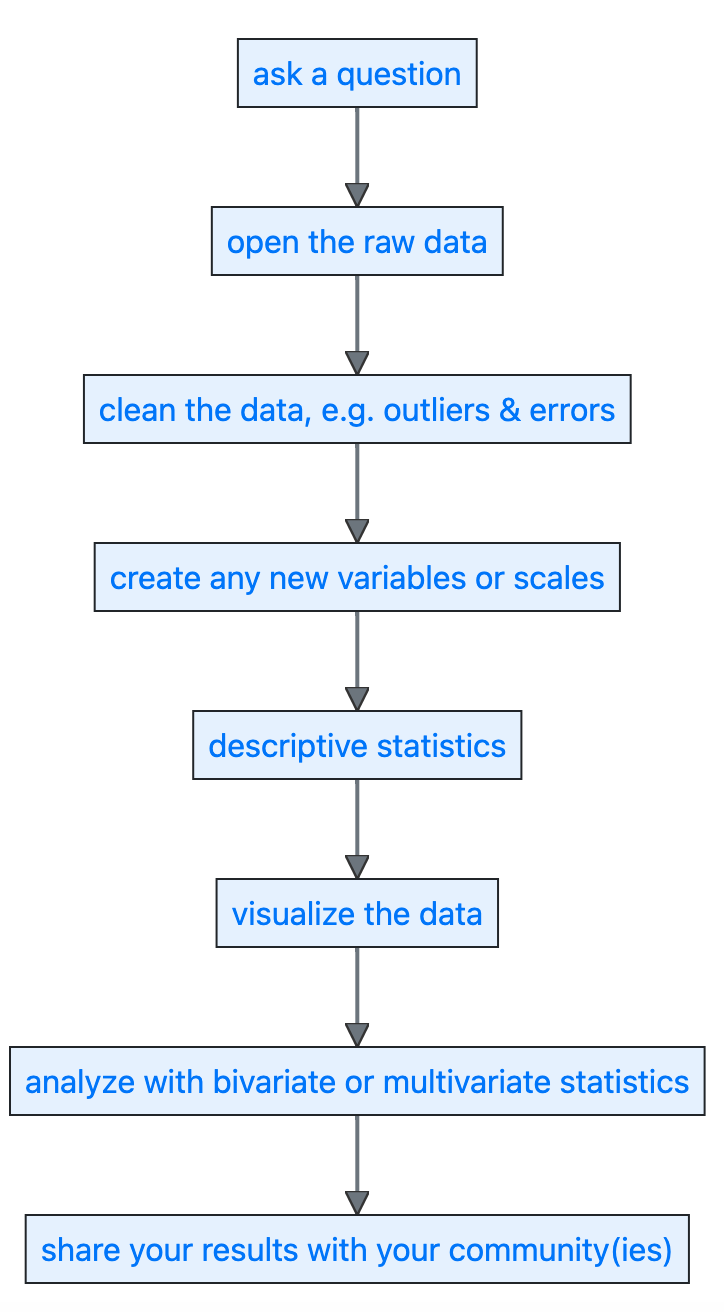
\includegraphics[width=0.33\textwidth,height=\textheight]{workflow.png}

}

\caption{A Common Statistical Workflow}

\end{figure}%

Increasingly, we want to think about workflows that are

\begin{itemize}
\tightlist
\item
  \textbf{documentable}, \textbf{transparent}, and \textbf{auditable}:
  We have a record of what we did if we want to double check our work,
  clarify a result, or develop a new project with a similar process. We,
  or others, can find the inevitable errors in our work, \textbf{and
  correct them}.
\item
  \textbf{replicable}: Others can replicate our findings with the same
  or new data.
\item
  \textbf{scalable}: We are developing a process that can be as easily
  used with \emph{thousands} or \emph{millions} of rows of data as it
  can with \emph{ten} rows of data. We are developing a process that can
  be easily repeated if we are \emph{constantly getting new or updated
  data}, e.g.~getting new data every week, or every month.
\end{itemize}

\section{Scripts}\label{scripts}

For most statistical workflows, we will often want to write a script or
code. Data analysis scripts can be stored in a Quarto document (Allaire
et al., 2024) as they are in this Appendix, or every statistical package
has its own unique format for storing scripts as a text file: in Stata,
scripts are stored in \texttt{.do} files; in R, scripts are stored in
\texttt{.R} files, and in Julia, scripts are stored in \texttt{.jl}
files.

\section{Script Flow}\label{sec-script-flow}

A good practice when writing a script, is to have a script that begins
with the raw data, moves through any necessary re-coding or cleaning of
the data, generates descriptive statistics, generates the appropriate
multivariate results, and then generates any necessary visualizations.

\section{Good Statistical Workflows Allow Multiple Statistical
Packages}\label{sec-multiple-packages}

While this Appendix focuses on the use of each individual statistical
package on its own, it is certainly possible to use multiple statistical
packages as part of the same workflow. For example, one might employ
Stata to carry out data management tasks, and then possibly use R to run
a multilevel model with a more complicated multilevel structure, such as
a cross-classified model, or Julia to more quickly run a model with a
large data.

\section{Good Statistical Workflows Require Safe
Workspaces}\label{good-statistical-workflows-require-safe-workspaces}

It is also \emph{very important} to be aware that good complex workflows
are \emph{highly iterative} and \emph{highly collaborative}. Good
complex workflows require a \emph{safe workspace} in which team members
feel free to admit their own errors, and help with others' mistakes in a
non-judgmental fashion. Such a \emph{safe environment} is necessary to
build an environment where the \emph{overall error rate} is low.

\section{Good Statistical Workflows Require Patience And Can Be
Psychologically
Demanding}\label{good-statistical-workflows-require-patience-and-can-be-psychologically-demanding}

Developing a good documented and auditable workflow that is implemented
in code requires a lot of patience, and often, \textbf{many iterations}.
Working through these many iterations can be psychologically demanding.
It is important to remember that careful attention to getting the
details right early in the research process, while sometimes tiring and
frustrating, will pay large dividends later on when the research is
reviewed, presented, published and read.

\section{Good Statistical Workflows Often Allow Multiple Principled Ways
Forward}\label{good-statistical-workflows-often-allow-multiple-principled-ways-forward}

One of my most recent ideas about statistical workflows is that there
are certainly \emph{wrong} decisions that one can make with data.

For example, I would not want to write the paper that says that smoking
prevents lung cancer, nor would I want to write a paper saying physical
punishment is good for children.

That being said, I think there are often \emph{multiple principled ways
forward}.

Often the key is not so much to make the 100\% correct decision, but to
make one of \emph{several possible principled decisions}.

Then after making a \emph{principled decision}, one is
\emph{transparent} and \emph{thorough} about describing the decision
that one made.

For example, in implementing a multilevel analysis, I would have many
choices: I could estimate only a random intercept; estimate one or more
random slopes; or estimate all possible random slopes. The random
effects could be correlated or uncorrelated. I could estimate only main
effects, or could estimate interactions of several variables. Each of
these would be a different, yet principled, approach to analyzing the
data.

In science and statistics, we often want an answer that provides one
clear direction. Instead, I'm increasingly convinced that the best
science (and teaching!) often involves engaging in open discussion about
the multiple possible alternatives, and then choosing one principled
solution, and being transparent about its implementation.

\bookmarksetup{startatroot}

\chapter{Storing Statistical Data}\label{storing-statistical-data}

\section{Spreadsheets}\label{spreadsheets}

Spreadsheets are sometimes used to collect and store data. Spreadsheets
may sometimes be used because they are the only program that some
individuals or agencies have for storing data. Spreadsheet programs may
also be used because spreadsheets can be very intuitive and easy ways of
managing small amounts of data.

However, spreadsheets may be problematic as an ultimate data storage
solution for a number of reasons detailed below, especially as data sets
grow in size. Notably, statistical programs like
\href{https://www.stata.com/}{Stata},
\href{https://www.r-project.org/}{R}, or
\href{https://julialang.org/}{Julia} can all store additional
information with each variable such as: a \emph{variable label},
describing the contents of the variable, or the survey question that
resulted in the variable; and a \emph{value label}, which attaches
qualitative information to each possible value of the response.

Spreadsheets do not generally contain this extra information about each
variable, or column of data, which may lead to errors in working with
quantitative information.

\begin{tcolorbox}[enhanced jigsaw, toptitle=1mm, title=\textcolor{quarto-callout-warning-color}{\faExclamationTriangle}\hspace{0.5em}{If Data Are Stored In A Spreadsheet, Variable Names Should Be Limited To
a Single Row of the Spreadsheet}, arc=.35mm, colbacktitle=quarto-callout-warning-color!10!white, left=2mm, breakable, toprule=.15mm, colback=white, opacityback=0, colframe=quarto-callout-warning-color-frame, leftrule=.75mm, opacitybacktitle=0.6, bottomtitle=1mm, titlerule=0mm, rightrule=.15mm, coltitle=black, bottomrule=.15mm]

If spreadsheets are used to store data, the first row of the data should
be used to list the variable names, as is seen in the example below.
Rows other than the first row should not contain additional information
about the variables, but should only contain data.

\begin{longtable}[]{@{}
  >{\centering\arraybackslash}p{(\columnwidth - 12\tabcolsep) * \real{0.1266}}
  >{\centering\arraybackslash}p{(\columnwidth - 12\tabcolsep) * \real{0.0759}}
  >{\centering\arraybackslash}p{(\columnwidth - 12\tabcolsep) * \real{0.1139}}
  >{\centering\arraybackslash}p{(\columnwidth - 12\tabcolsep) * \real{0.0759}}
  >{\centering\arraybackslash}p{(\columnwidth - 12\tabcolsep) * \real{0.1392}}
  >{\centering\arraybackslash}p{(\columnwidth - 12\tabcolsep) * \real{0.1899}}
  >{\centering\arraybackslash}p{(\columnwidth - 12\tabcolsep) * \real{0.2785}}@{}}

\caption{\label{tbl-spreadsheet}Example Data As Stored in A Spreadsheet}

\tabularnewline

\caption{Table continues below}\tabularnewline
\toprule\noalign{}
\begin{minipage}[b]{\linewidth}\centering
country
\end{minipage} & \begin{minipage}[b]{\linewidth}\centering
HDI
\end{minipage} & \begin{minipage}[b]{\linewidth}\centering
family
\end{minipage} & \begin{minipage}[b]{\linewidth}\centering
id
\end{minipage} & \begin{minipage}[b]{\linewidth}\centering
identity
\end{minipage} & \begin{minipage}[b]{\linewidth}\centering
intervention
\end{minipage} & \begin{minipage}[b]{\linewidth}\centering
physical\_punishment
\end{minipage} \\
\midrule\noalign{}
\endfirsthead
\toprule\noalign{}
\begin{minipage}[b]{\linewidth}\centering
country
\end{minipage} & \begin{minipage}[b]{\linewidth}\centering
HDI
\end{minipage} & \begin{minipage}[b]{\linewidth}\centering
family
\end{minipage} & \begin{minipage}[b]{\linewidth}\centering
id
\end{minipage} & \begin{minipage}[b]{\linewidth}\centering
identity
\end{minipage} & \begin{minipage}[b]{\linewidth}\centering
intervention
\end{minipage} & \begin{minipage}[b]{\linewidth}\centering
physical\_punishment
\end{minipage} \\
\midrule\noalign{}
\endhead
\bottomrule\noalign{}
\endlastfoot
1 & 69 & 1 & 1.1 & 1 & 0 & 3 \\
1 & 69 & 2 & 1.2 & 1 & 1 & 2 \\
1 & 69 & 3 & 1.3 & 0 & 1 & 3 \\
1 & 69 & 4 & 1.4 & 1 & 0 & 0 \\
1 & 69 & 5 & 1.5 & 1 & 0 & 4 \\
1 & 69 & 6 & 1.6 & 0 & 1 & 5 \\

\end{longtable}

\begin{longtable}[]{@{}
  >{\centering\arraybackslash}p{(\columnwidth - 2\tabcolsep) * \real{0.1250}}
  >{\centering\arraybackslash}p{(\columnwidth - 2\tabcolsep) * \real{0.1389}}@{}}

\caption{\label{tbl-spreadsheet}Example Data As Stored in A Spreadsheet}

\tabularnewline

\toprule\noalign{}
\begin{minipage}[b]{\linewidth}\centering
warmth
\end{minipage} & \begin{minipage}[b]{\linewidth}\centering
outcome
\end{minipage} \\
\midrule\noalign{}
\endhead
\bottomrule\noalign{}
\endlastfoot
3 & 57.47 \\
1 & 50.1 \\
2 & 52.92 \\
5 & 60.17 \\
4 & 55.05 \\
3 & 49.81 \\

\end{longtable}

\end{tcolorbox}

\section{Data in Statistical Format}\label{data-in-statistical-format}

I load the data from a statistical program.

\subsection{Describe The Data}\label{describe-the-data}

Notice how a description of the data contains information that helps us
to understand the variables.

\begin{longtable}[]{@{}
  >{\centering\arraybackslash}p{(\columnwidth - 4\tabcolsep) * \real{0.0833}}
  >{\centering\arraybackslash}p{(\columnwidth - 4\tabcolsep) * \real{0.3056}}
  >{\centering\arraybackslash}p{(\columnwidth - 4\tabcolsep) * \real{0.4306}}@{}}

\caption{\label{tbl-varlabels}Variable Labels}

\tabularnewline

\toprule\noalign{}
\begin{minipage}[b]{\linewidth}\centering
pos
\end{minipage} & \begin{minipage}[b]{\linewidth}\centering
variable
\end{minipage} & \begin{minipage}[b]{\linewidth}\centering
label
\end{minipage} \\
\midrule\noalign{}
\endhead
\bottomrule\noalign{}
\endlastfoot
1 & country & country id \\
2 & HDI & Human Development Index \\
3 & family & family id \\
4 & id & unique country family id \\
5 & identity & hypothetical identity group variable \\
6 & intervention & recieved intervention \\
7 & physical\_punishment & physical punishment in past week \\
8 & warmth & parental warmth in past week \\
9 & outcome & beneficial outcome \\

\end{longtable}

\subsection{Descriptive Statistics}\label{descriptive-statistics}

\begin{tcolorbox}[enhanced jigsaw, toptitle=1mm, title=\textcolor{quarto-callout-tip-color}{\faLightbulb}\hspace{0.5em}{Variable Labels and Value Labels Help Us Understand Our Data}, arc=.35mm, colbacktitle=quarto-callout-tip-color!10!white, left=2mm, breakable, toprule=.15mm, colback=white, opacityback=0, colframe=quarto-callout-tip-color-frame, leftrule=.75mm, opacitybacktitle=0.6, bottomtitle=1mm, titlerule=0mm, rightrule=.15mm, coltitle=black, bottomrule=.15mm]

Notice how the descriptive statistics and graph are informative in that
they contain information on the \emph{variable label} and \emph{value
label}. These help us to get an intuitive sense of the information in
the data. We see this information when we list out the data as well.

\end{tcolorbox}

\begin{longtable}[]{@{}
  >{\centering\arraybackslash}p{(\columnwidth - 6\tabcolsep) * \real{0.2083}}
  >{\centering\arraybackslash}p{(\columnwidth - 6\tabcolsep) * \real{0.2222}}
  >{\centering\arraybackslash}p{(\columnwidth - 6\tabcolsep) * \real{0.2361}}
  >{\centering\arraybackslash}p{(\columnwidth - 6\tabcolsep) * \real{0.2639}}@{}}

\caption{\label{tbl-descriptives}Descriptive Statistics}

\tabularnewline

\caption{Table continues below}\tabularnewline
\toprule\noalign{}
\begin{minipage}[b]{\linewidth}\centering
country
\end{minipage} & \begin{minipage}[b]{\linewidth}\centering
HDI
\end{minipage} & \begin{minipage}[b]{\linewidth}\centering
family
\end{minipage} & \begin{minipage}[b]{\linewidth}\centering
id
\end{minipage} \\
\midrule\noalign{}
\endfirsthead
\toprule\noalign{}
\begin{minipage}[b]{\linewidth}\centering
country
\end{minipage} & \begin{minipage}[b]{\linewidth}\centering
HDI
\end{minipage} & \begin{minipage}[b]{\linewidth}\centering
family
\end{minipage} & \begin{minipage}[b]{\linewidth}\centering
id
\end{minipage} \\
\midrule\noalign{}
\endhead
\bottomrule\noalign{}
\endlastfoot
1 : 100 & Min. :33.00 & Min. : 1.00 & Length:3000 \\
2 : 100 & 1st Qu.:53.00 & 1st Qu.: 25.75 & Class :character \\
3 : 100 & Median :70.00 & Median : 50.50 & Mode :character \\
4 : 100 & Mean :64.77 & Mean : 50.50 & NA \\
5 : 100 & 3rd Qu.:81.00 & 3rd Qu.: 75.25 & NA \\
6 : 100 & Max. :87.00 & Max. :100.00 & NA \\
(Other):2400 & NA & NA & NA \\

\end{longtable}

\begin{longtable}[]{@{}
  >{\centering\arraybackslash}p{(\columnwidth - 6\tabcolsep) * \real{0.2278}}
  >{\centering\arraybackslash}p{(\columnwidth - 6\tabcolsep) * \real{0.2911}}
  >{\centering\arraybackslash}p{(\columnwidth - 6\tabcolsep) * \real{0.2785}}
  >{\centering\arraybackslash}p{(\columnwidth - 6\tabcolsep) * \real{0.2025}}@{}}

\caption{\label{tbl-descriptives}Descriptive Statistics}

\tabularnewline

\caption{Table continues below}\tabularnewline
\toprule\noalign{}
\begin{minipage}[b]{\linewidth}\centering
identity
\end{minipage} & \begin{minipage}[b]{\linewidth}\centering
intervention
\end{minipage} & \begin{minipage}[b]{\linewidth}\centering
physical\_punishment
\end{minipage} & \begin{minipage}[b]{\linewidth}\centering
warmth
\end{minipage} \\
\midrule\noalign{}
\endfirsthead
\toprule\noalign{}
\begin{minipage}[b]{\linewidth}\centering
identity
\end{minipage} & \begin{minipage}[b]{\linewidth}\centering
intervention
\end{minipage} & \begin{minipage}[b]{\linewidth}\centering
physical\_punishment
\end{minipage} & \begin{minipage}[b]{\linewidth}\centering
warmth
\end{minipage} \\
\midrule\noalign{}
\endhead
\bottomrule\noalign{}
\endlastfoot
Identity B:1507 & no intervention:1547 & Min. :0.000 & Min. :0.000 \\
Identity A:1493 & intervention :1453 & 1st Qu.:2.000 & 1st Qu.:2.000 \\
NA & NA & Median :2.000 & Median :4.000 \\
NA & NA & Mean :2.479 & Mean :3.522 \\
NA & NA & 3rd Qu.:3.000 & 3rd Qu.:5.000 \\
NA & NA & Max. :5.000 & Max. :7.000 \\
NA & NA & NA & NA \\

\end{longtable}

\begin{longtable}[]{@{}
  >{\centering\arraybackslash}p{(\columnwidth - 0\tabcolsep) * \real{0.2222}}@{}}

\caption{\label{tbl-descriptives}Descriptive Statistics}

\tabularnewline

\toprule\noalign{}
\begin{minipage}[b]{\linewidth}\centering
outcome
\end{minipage} \\
\midrule\noalign{}
\endhead
\bottomrule\noalign{}
\endlastfoot
Min. :29.61 \\
1st Qu.:48.02 \\
Median :52.45 \\
Mean :52.43 \\
3rd Qu.:56.86 \\
Max. :74.84 \\
NA \\

\end{longtable}

\subsection{Graph}\label{graph}

\begin{figure}

\centering{

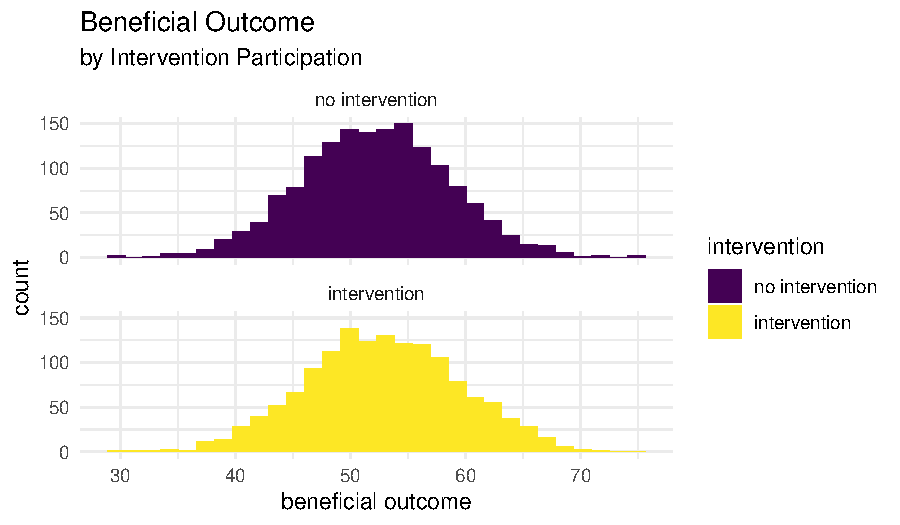
\includegraphics{storage-multilingual_files/figure-pdf/fig-graph-statistical-1.pdf}

}

\caption{\label{fig-graph-statistical}Graph from Data Stored in
Statistical Software}

\end{figure}%

\subsection{List Out A Sample Of The
Data}\label{list-out-a-sample-of-the-data}

\begin{longtable}[]{@{}
  >{\centering\arraybackslash}p{(\columnwidth - 10\tabcolsep) * \real{0.1389}}
  >{\centering\arraybackslash}p{(\columnwidth - 10\tabcolsep) * \real{0.0833}}
  >{\centering\arraybackslash}p{(\columnwidth - 10\tabcolsep) * \real{0.1250}}
  >{\centering\arraybackslash}p{(\columnwidth - 10\tabcolsep) * \real{0.0833}}
  >{\centering\arraybackslash}p{(\columnwidth - 10\tabcolsep) * \real{0.1806}}
  >{\centering\arraybackslash}p{(\columnwidth - 10\tabcolsep) * \real{0.2500}}@{}}

\caption{\label{tbl-head}Sample of Data}

\tabularnewline

\caption{Table continues below}\tabularnewline
\toprule\noalign{}
\begin{minipage}[b]{\linewidth}\centering
country
\end{minipage} & \begin{minipage}[b]{\linewidth}\centering
HDI
\end{minipage} & \begin{minipage}[b]{\linewidth}\centering
family
\end{minipage} & \begin{minipage}[b]{\linewidth}\centering
id
\end{minipage} & \begin{minipage}[b]{\linewidth}\centering
identity
\end{minipage} & \begin{minipage}[b]{\linewidth}\centering
intervention
\end{minipage} \\
\midrule\noalign{}
\endfirsthead
\toprule\noalign{}
\begin{minipage}[b]{\linewidth}\centering
country
\end{minipage} & \begin{minipage}[b]{\linewidth}\centering
HDI
\end{minipage} & \begin{minipage}[b]{\linewidth}\centering
family
\end{minipage} & \begin{minipage}[b]{\linewidth}\centering
id
\end{minipage} & \begin{minipage}[b]{\linewidth}\centering
identity
\end{minipage} & \begin{minipage}[b]{\linewidth}\centering
intervention
\end{minipage} \\
\midrule\noalign{}
\endhead
\bottomrule\noalign{}
\endlastfoot
1 & 69 & 1 & 1.1 & Identity A & no intervention \\
1 & 69 & 2 & 1.2 & Identity A & intervention \\
1 & 69 & 3 & 1.3 & Identity B & intervention \\
1 & 69 & 4 & 1.4 & Identity A & no intervention \\
1 & 69 & 5 & 1.5 & Identity A & no intervention \\
1 & 69 & 6 & 1.6 & Identity B & intervention \\

\end{longtable}

\begin{longtable}[]{@{}
  >{\centering\arraybackslash}p{(\columnwidth - 4\tabcolsep) * \real{0.3056}}
  >{\centering\arraybackslash}p{(\columnwidth - 4\tabcolsep) * \real{0.1250}}
  >{\centering\arraybackslash}p{(\columnwidth - 4\tabcolsep) * \real{0.1389}}@{}}

\caption{\label{tbl-head}Sample of Data}

\tabularnewline

\toprule\noalign{}
\begin{minipage}[b]{\linewidth}\centering
physical\_punishment
\end{minipage} & \begin{minipage}[b]{\linewidth}\centering
warmth
\end{minipage} & \begin{minipage}[b]{\linewidth}\centering
outcome
\end{minipage} \\
\midrule\noalign{}
\endhead
\bottomrule\noalign{}
\endlastfoot
3 & 3 & 57.47 \\
2 & 1 & 50.1 \\
3 & 2 & 52.92 \\
0 & 5 & 60.17 \\
4 & 4 & 55.05 \\
5 & 3 & 49.81 \\

\end{longtable}

\section{Data In Spreadsheet Format}\label{data-in-spreadsheet-format}

I now import the spreadsheet data file. I use the first row of data as
variable names.

We see right away that the data are less informative.

\subsection{Describe The Data}\label{describe-the-data-1}

Notice how a description of the data no longer contains much of the
information that helped us to understand the variables.

\begin{longtable}[]{@{}
  >{\centering\arraybackslash}p{(\columnwidth - 4\tabcolsep) * \real{0.0833}}
  >{\centering\arraybackslash}p{(\columnwidth - 4\tabcolsep) * \real{0.3056}}
  >{\centering\arraybackslash}p{(\columnwidth - 4\tabcolsep) * \real{0.1111}}@{}}

\caption{\label{tbl-varlabels2}Example Data As Stored in A Spreadsheet}

\tabularnewline

\toprule\noalign{}
\begin{minipage}[b]{\linewidth}\centering
pos
\end{minipage} & \begin{minipage}[b]{\linewidth}\centering
variable
\end{minipage} & \begin{minipage}[b]{\linewidth}\centering
label
\end{minipage} \\
\midrule\noalign{}
\endhead
\bottomrule\noalign{}
\endlastfoot
1 & country & NA \\
2 & HDI & NA \\
3 & family & NA \\
4 & id & NA \\
5 & identity & NA \\
6 & intervention & NA \\
7 & physical\_punishment & NA \\
8 & warmth & NA \\
9 & outcome & NA \\

\end{longtable}

\begin{longtable}[]{@{}
  >{\centering\arraybackslash}p{(\columnwidth - 12\tabcolsep) * \real{0.1266}}
  >{\centering\arraybackslash}p{(\columnwidth - 12\tabcolsep) * \real{0.0759}}
  >{\centering\arraybackslash}p{(\columnwidth - 12\tabcolsep) * \real{0.1139}}
  >{\centering\arraybackslash}p{(\columnwidth - 12\tabcolsep) * \real{0.0759}}
  >{\centering\arraybackslash}p{(\columnwidth - 12\tabcolsep) * \real{0.1392}}
  >{\centering\arraybackslash}p{(\columnwidth - 12\tabcolsep) * \real{0.1899}}
  >{\centering\arraybackslash}p{(\columnwidth - 12\tabcolsep) * \real{0.2785}}@{}}

\caption{\label{tbl-spreadsheet2}Example Data As Stored in A
Spreadsheet}

\tabularnewline

\caption{Table continues below}\tabularnewline
\toprule\noalign{}
\begin{minipage}[b]{\linewidth}\centering
country
\end{minipage} & \begin{minipage}[b]{\linewidth}\centering
HDI
\end{minipage} & \begin{minipage}[b]{\linewidth}\centering
family
\end{minipage} & \begin{minipage}[b]{\linewidth}\centering
id
\end{minipage} & \begin{minipage}[b]{\linewidth}\centering
identity
\end{minipage} & \begin{minipage}[b]{\linewidth}\centering
intervention
\end{minipage} & \begin{minipage}[b]{\linewidth}\centering
physical\_punishment
\end{minipage} \\
\midrule\noalign{}
\endfirsthead
\toprule\noalign{}
\begin{minipage}[b]{\linewidth}\centering
country
\end{minipage} & \begin{minipage}[b]{\linewidth}\centering
HDI
\end{minipage} & \begin{minipage}[b]{\linewidth}\centering
family
\end{minipage} & \begin{minipage}[b]{\linewidth}\centering
id
\end{minipage} & \begin{minipage}[b]{\linewidth}\centering
identity
\end{minipage} & \begin{minipage}[b]{\linewidth}\centering
intervention
\end{minipage} & \begin{minipage}[b]{\linewidth}\centering
physical\_punishment
\end{minipage} \\
\midrule\noalign{}
\endhead
\bottomrule\noalign{}
\endlastfoot
1 & 69 & 1 & 1.1 & 1 & 0 & 3 \\
1 & 69 & 2 & 1.2 & 1 & 1 & 2 \\
1 & 69 & 3 & 1.3 & 0 & 1 & 3 \\
1 & 69 & 4 & 1.4 & 1 & 0 & 0 \\
1 & 69 & 5 & 1.5 & 1 & 0 & 4 \\
1 & 69 & 6 & 1.6 & 0 & 1 & 5 \\

\end{longtable}

\begin{longtable}[]{@{}
  >{\centering\arraybackslash}p{(\columnwidth - 2\tabcolsep) * \real{0.1250}}
  >{\centering\arraybackslash}p{(\columnwidth - 2\tabcolsep) * \real{0.1389}}@{}}

\caption{\label{tbl-spreadsheet2}Example Data As Stored in A
Spreadsheet}

\tabularnewline

\toprule\noalign{}
\begin{minipage}[b]{\linewidth}\centering
warmth
\end{minipage} & \begin{minipage}[b]{\linewidth}\centering
outcome
\end{minipage} \\
\midrule\noalign{}
\endhead
\bottomrule\noalign{}
\endlastfoot
3 & 57.47 \\
1 & 50.1 \\
2 & 52.92 \\
5 & 60.17 \\
4 & 55.05 \\
3 & 49.81 \\

\end{longtable}

\begin{tcolorbox}[enhanced jigsaw, toptitle=1mm, title=\textcolor{quarto-callout-warning-color}{\faExclamationTriangle}\hspace{0.5em}{Warning}, arc=.35mm, colbacktitle=quarto-callout-warning-color!10!white, left=2mm, breakable, toprule=.15mm, colback=white, opacityback=0, colframe=quarto-callout-warning-color-frame, leftrule=.75mm, opacitybacktitle=0.6, bottomtitle=1mm, titlerule=0mm, rightrule=.15mm, coltitle=black, bottomrule=.15mm]

Adding this valuable information back into the data set may take a great
deal of extra effort.

\end{tcolorbox}

\subsection{Descriptive Statistics}\label{descriptive-statistics-1}

Notice here how the descriptive statistics and graph are much less
informative. For example, it is now not immediately clear what the
values of \texttt{identity} or \texttt{intervention} represent. The
information on variable labels and value labels will have to be added
back into the data when preparing a final product for dissemination.

\begin{longtable}[]{@{}
  >{\centering\arraybackslash}p{(\columnwidth - 6\tabcolsep) * \real{0.2083}}
  >{\centering\arraybackslash}p{(\columnwidth - 6\tabcolsep) * \real{0.2222}}
  >{\centering\arraybackslash}p{(\columnwidth - 6\tabcolsep) * \real{0.2361}}
  >{\centering\arraybackslash}p{(\columnwidth - 6\tabcolsep) * \real{0.2639}}@{}}

\caption{\label{tbl-descriptives2}Descriptive Statistics}

\tabularnewline

\caption{Table continues below}\tabularnewline
\toprule\noalign{}
\begin{minipage}[b]{\linewidth}\centering
country
\end{minipage} & \begin{minipage}[b]{\linewidth}\centering
HDI
\end{minipage} & \begin{minipage}[b]{\linewidth}\centering
family
\end{minipage} & \begin{minipage}[b]{\linewidth}\centering
id
\end{minipage} \\
\midrule\noalign{}
\endfirsthead
\toprule\noalign{}
\begin{minipage}[b]{\linewidth}\centering
country
\end{minipage} & \begin{minipage}[b]{\linewidth}\centering
HDI
\end{minipage} & \begin{minipage}[b]{\linewidth}\centering
family
\end{minipage} & \begin{minipage}[b]{\linewidth}\centering
id
\end{minipage} \\
\midrule\noalign{}
\endhead
\bottomrule\noalign{}
\endlastfoot
Min. : 1.0 & Min. :33.00 & Min. : 1.00 & Length:3000 \\
1st Qu.: 8.0 & 1st Qu.:53.00 & 1st Qu.: 25.75 & Class :character \\
Median :15.5 & Median :70.00 & Median : 50.50 & Mode :character \\
Mean :15.5 & Mean :64.77 & Mean : 50.50 & NA \\
3rd Qu.:23.0 & 3rd Qu.:81.00 & 3rd Qu.: 75.25 & NA \\
Max. :30.0 & Max. :87.00 & Max. :100.00 & NA \\

\end{longtable}

\begin{longtable}[]{@{}
  >{\centering\arraybackslash}p{(\columnwidth - 6\tabcolsep) * \real{0.2361}}
  >{\centering\arraybackslash}p{(\columnwidth - 6\tabcolsep) * \real{0.2361}}
  >{\centering\arraybackslash}p{(\columnwidth - 6\tabcolsep) * \real{0.3056}}
  >{\centering\arraybackslash}p{(\columnwidth - 6\tabcolsep) * \real{0.2222}}@{}}

\caption{\label{tbl-descriptives2}Descriptive Statistics}

\tabularnewline

\caption{Table continues below}\tabularnewline
\toprule\noalign{}
\begin{minipage}[b]{\linewidth}\centering
identity
\end{minipage} & \begin{minipage}[b]{\linewidth}\centering
intervention
\end{minipage} & \begin{minipage}[b]{\linewidth}\centering
physical\_punishment
\end{minipage} & \begin{minipage}[b]{\linewidth}\centering
warmth
\end{minipage} \\
\midrule\noalign{}
\endfirsthead
\toprule\noalign{}
\begin{minipage}[b]{\linewidth}\centering
identity
\end{minipage} & \begin{minipage}[b]{\linewidth}\centering
intervention
\end{minipage} & \begin{minipage}[b]{\linewidth}\centering
physical\_punishment
\end{minipage} & \begin{minipage}[b]{\linewidth}\centering
warmth
\end{minipage} \\
\midrule\noalign{}
\endhead
\bottomrule\noalign{}
\endlastfoot
Min. :0.0000 & Min. :0.0000 & Min. :0.000 & Min. :0.000 \\
1st Qu.:0.0000 & 1st Qu.:0.0000 & 1st Qu.:2.000 & 1st Qu.:2.000 \\
Median :0.0000 & Median :0.0000 & Median :2.000 & Median :4.000 \\
Mean :0.4977 & Mean :0.4843 & Mean :2.479 & Mean :3.522 \\
3rd Qu.:1.0000 & 3rd Qu.:1.0000 & 3rd Qu.:3.000 & 3rd Qu.:5.000 \\
Max. :1.0000 & Max. :1.0000 & Max. :5.000 & Max. :7.000 \\

\end{longtable}

\begin{longtable}[]{@{}
  >{\centering\arraybackslash}p{(\columnwidth - 0\tabcolsep) * \real{0.2222}}@{}}

\caption{\label{tbl-descriptives2}Descriptive Statistics}

\tabularnewline

\toprule\noalign{}
\begin{minipage}[b]{\linewidth}\centering
outcome
\end{minipage} \\
\midrule\noalign{}
\endhead
\bottomrule\noalign{}
\endlastfoot
Min. :29.61 \\
1st Qu.:48.02 \\
Median :52.45 \\
Mean :52.43 \\
3rd Qu.:56.86 \\
Max. :74.84 \\

\end{longtable}

\subsection{Graph}\label{graph-1}

While the graph has an informative title, as well as informative axis
labels, a crucial piece of information is missing: what each status of
the intervention represents.

\begin{figure}

\centering{

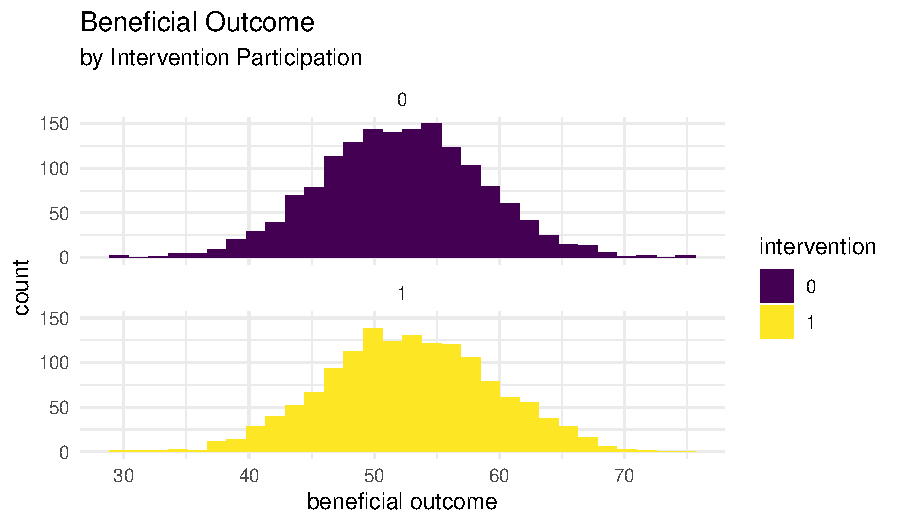
\includegraphics{storage-multilingual_files/figure-pdf/fig-graph-spreadsheet-1.pdf}

}

\caption{\label{fig-graph-spreadsheet}Graph from Data Stored in
Spreadsheet}

\end{figure}%

\section{A Few Final Issues}\label{a-few-final-issues}

Notice, finally, how spreadsheets don't enforce the idea of whether
variables are \emph{numeric}, or \emph{text}, and so would allow storage
of different types of information in the same column. Relatedly,
\emph{numeric} variables may be improperly stored as \emph{text}, often
necessitating recoding before graphical or statistical procedures can be
employed.

Second, a spreadsheet would allow some of your columns to have the same
name, which might make data difficult to work with in other software.

Lastly, spreadsheets do not enforce the idea that the data have a
\emph{structure} wherein the \emph{column header} is a \emph{variable
name}, while the \emph{other rows} are \emph{data}.

\begin{longtable}[]{@{}
  >{\raggedright\arraybackslash}p{(\columnwidth - 6\tabcolsep) * \real{0.1667}}
  >{\raggedright\arraybackslash}p{(\columnwidth - 6\tabcolsep) * \real{0.1111}}
  >{\raggedright\arraybackslash}p{(\columnwidth - 6\tabcolsep) * \real{0.3194}}
  >{\raggedright\arraybackslash}p{(\columnwidth - 6\tabcolsep) * \real{0.3611}}@{}}
\caption{A Spreadsheet Table With Problematic
Organization}\label{tbl-problematic}\tabularnewline
\toprule\noalign{}
\begin{minipage}[b]{\linewidth}\raggedright
x
\end{minipage} & \begin{minipage}[b]{\linewidth}\raggedright
y
\end{minipage} & \begin{minipage}[b]{\linewidth}\raggedright
verylongvariablename
\end{minipage} & \begin{minipage}[b]{\linewidth}\raggedright
verylongvariablename
\end{minipage} \\
\midrule\noalign{}
\endfirsthead
\toprule\noalign{}
\begin{minipage}[b]{\linewidth}\raggedright
x
\end{minipage} & \begin{minipage}[b]{\linewidth}\raggedright
y
\end{minipage} & \begin{minipage}[b]{\linewidth}\raggedright
verylongvariablename
\end{minipage} & \begin{minipage}[b]{\linewidth}\raggedright
verylongvariablename
\end{minipage} \\
\midrule\noalign{}
\endhead
\bottomrule\noalign{}
\endlastfoot
100 & 1 & Smith & 20 \\
200 & 2 & 30 & NA \\
not applicable & x & yes & 60 \\
& & some other random information & \\
\end{longtable}

\section{File Organization}\label{file-organization}

Files for all of your work should not be stored all together in
\texttt{downloads}. Ideally, you should have a specific set of folders
for your work. Each project, should be stored in its own individual
folder. Ideally, each project folder would have a separate sub-folder
for separate aspects of the project such as data, code or syntax, and
various outputs.

\begin{figure}[H]

{\centering 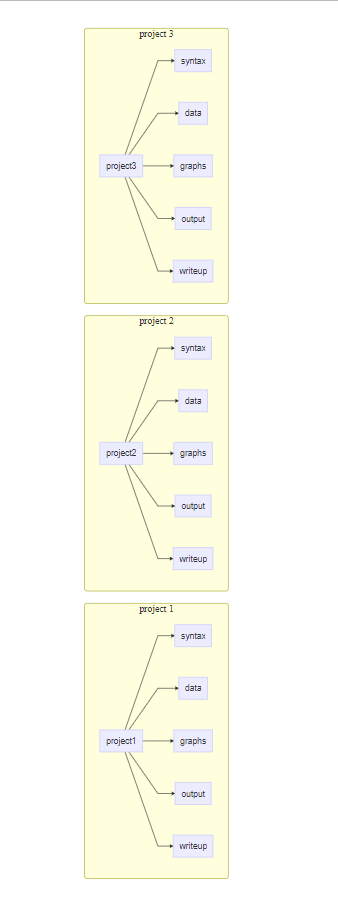
\includegraphics{storage.png}

}

\caption{A Hypothetical Set of Folders and Subfolders}

\end{figure}%

\bookmarksetup{startatroot}

\chapter{Descriptive Statistics}\label{descriptive-statistics-2}

\section{Descriptive Statistics}\label{descriptive-statistics-3}

\subsection{Stata}

\begin{Shaded}
\begin{Highlighting}[]

\KeywordTok{use}\NormalTok{ simulated\_multilevel\_data.dta }\CommentTok{// use data}
\end{Highlighting}
\end{Shaded}

We use \texttt{summarize} for \emph{continuous} variables, and
\texttt{tabulate} for \emph{categorical} variables.

\begin{Shaded}
\begin{Highlighting}[]
\KeywordTok{summarize}\NormalTok{ outcome warmth physical\_punishment HDI}

\KeywordTok{tabulate} \KeywordTok{identity}

\KeywordTok{tabulate}\NormalTok{ intervention}
\end{Highlighting}
\end{Shaded}

\begin{verbatim}
    Variable |        Obs        Mean    Std. dev.       Min        Max
-------------+---------------------------------------------------------
     outcome |      3,000    52.43327    6.530996   29.60798   74.83553
      warmth |      3,000    3.521667    1.888399          0          7
physical_p~t |      3,000    2.478667    1.360942          0          5
         HDI |      3,000    64.76667    17.24562         33         87


hypothetica |
 l identity |
      group |
   variable |      Freq.     Percent        Cum.
------------+-----------------------------------
          0 |      1,507       50.23       50.23
          1 |      1,493       49.77      100.00
------------+-----------------------------------
      Total |      3,000      100.00


   recieved |
interventio |
          n |      Freq.     Percent        Cum.
------------+-----------------------------------
          0 |      1,547       51.57       51.57
          1 |      1,453       48.43      100.00
------------+-----------------------------------
      Total |      3,000      100.00
\end{verbatim}

\subsection{R}

\begin{Shaded}
\begin{Highlighting}[]
\FunctionTok{library}\NormalTok{(haven) }\CommentTok{\# read data in Stata format}

\NormalTok{df }\OtherTok{\textless{}{-}} \FunctionTok{read\_dta}\NormalTok{(}\StringTok{"simulated\_multilevel\_data.dta"}\NormalTok{)}
\end{Highlighting}
\end{Shaded}

R's descriptive statistics functions rely heavily on whether a variable
is a \emph{numeric} variable, or a \emph{factor} variable. Below, I
convert two variables to factors (\texttt{factor}) before using
\texttt{summary}\footnote{\texttt{skimr} is an excellent new alternative
  library for generating descriptive statistics in R.} to generate
descriptive statistics.

\begin{Shaded}
\begin{Highlighting}[]
\NormalTok{df}\SpecialCharTok{$}\NormalTok{country }\OtherTok{\textless{}{-}} \FunctionTok{factor}\NormalTok{(df}\SpecialCharTok{$}\NormalTok{country)}

\NormalTok{df}\SpecialCharTok{$}\NormalTok{identity }\OtherTok{\textless{}{-}} \FunctionTok{factor}\NormalTok{(df}\SpecialCharTok{$}\NormalTok{identity)}

\NormalTok{df}\SpecialCharTok{$}\NormalTok{intervention }\OtherTok{\textless{}{-}} \FunctionTok{factor}\NormalTok{(df}\SpecialCharTok{$}\NormalTok{intervention)}

\FunctionTok{summary}\NormalTok{(df)}
\end{Highlighting}
\end{Shaded}

\begin{verbatim}
    country          HDI            family            id            identity
 1      : 100   Min.   :33.00   Min.   :  1.00   Length:3000        0:1507  
 2      : 100   1st Qu.:53.00   1st Qu.: 25.75   Class :character   1:1493  
 3      : 100   Median :70.00   Median : 50.50   Mode  :character           
 4      : 100   Mean   :64.77   Mean   : 50.50                              
 5      : 100   3rd Qu.:81.00   3rd Qu.: 75.25                              
 6      : 100   Max.   :87.00   Max.   :100.00                              
 (Other):2400                                                               
 intervention physical_punishment     warmth         outcome     
 0:1547       Min.   :0.000       Min.   :0.000   Min.   :29.61  
 1:1453       1st Qu.:2.000       1st Qu.:2.000   1st Qu.:48.02  
              Median :2.000       Median :4.000   Median :52.45  
              Mean   :2.479       Mean   :3.522   Mean   :52.43  
              3rd Qu.:3.000       3rd Qu.:5.000   3rd Qu.:56.86  
              Max.   :5.000       Max.   :7.000   Max.   :74.84  
                                                                 
\end{verbatim}

\subsection{Julia}

\begin{Shaded}
\begin{Highlighting}[]
\ImportTok{using} \BuiltInTok{Tables}\NormalTok{, }\BuiltInTok{MixedModels}\NormalTok{, }\BuiltInTok{MixedModelsExtras}\NormalTok{, }\BuiltInTok{StatFiles}\NormalTok{, }\BuiltInTok{DataFrames}\NormalTok{, }\BuiltInTok{CategoricalArrays}\NormalTok{, }\BuiltInTok{DataFramesMeta}

\NormalTok{df }\OperatorTok{=} \FunctionTok{DataFrame}\NormalTok{(}\FunctionTok{load}\NormalTok{(}\StringTok{"simulated\_multilevel\_data.dta"}\NormalTok{))}
\end{Highlighting}
\end{Shaded}

Similarly to R, Julia relies on the idea of \emph{variable type}. I use
\texttt{transform} to convert the appropriate variables to
\emph{categorical} variables.

\begin{Shaded}
\begin{Highlighting}[]
\PreprocessorTok{@transform}\NormalTok{!(df, }\OperatorTok{:}\NormalTok{country }\OperatorTok{=} \FunctionTok{categorical}\NormalTok{(}\OperatorTok{:}\NormalTok{country))}

\PreprocessorTok{@transform}\NormalTok{!(df, }\OperatorTok{:}\NormalTok{identity }\OperatorTok{=} \FunctionTok{categorical}\NormalTok{(}\OperatorTok{:}\NormalTok{identity))}

\PreprocessorTok{@transform}\NormalTok{!(df, }\OperatorTok{:}\NormalTok{intervention }\OperatorTok{=} \FunctionTok{categorical}\NormalTok{(}\OperatorTok{:}\NormalTok{intervention))}
\end{Highlighting}
\end{Shaded}

\begin{Shaded}
\begin{Highlighting}[]

\FunctionTok{describe}\NormalTok{(df) }\CommentTok{\# descriptive statistics}
\end{Highlighting}
\end{Shaded}

\begin{verbatim}
9×7 DataFrame
 Row │ variable             mean     min     median  max      nmissing  eltype ⋯
     │ Symbol               Union…   Any     Union…  Any      Int64     Union  ⋯
─────┼──────────────────────────────────────────────────────────────────────────
   1 │ country                       1.0             30.0            0  Union{ ⋯
   2 │ HDI                  64.7667  33.0    70.0    87.0            0  Union{
   3 │ family               50.5     1.0     50.5    100.0           0  Union{
   4 │ id                            1.1             9.99            0  Union{
   5 │ identity                      0.0             1.0             0  Union{ ⋯
   6 │ intervention                  0.0             1.0             0  Union{
   7 │ physical_punishment  2.47867  0.0     2.0     5.0             0  Union{
   8 │ warmth               3.52167  0.0     4.0     7.0             0  Union{
   9 │ outcome              52.4333  29.608  52.449  74.8355         0  Union{ ⋯
                                                                1 column omitted
\end{verbatim}

\section{Interpretation}\label{interpretation}

Examining descriptive statistics is an important first step in any
analysis. It is important to examine your descriptive statistics before
skipping ahead to more sophisticated analyses, such as multilevel
models.

In examining the descriptive statistics for this data, we get a sense of
the data.

\begin{itemize}
\tightlist
\item
  \texttt{outcome} has a mean of approximately 52 and ranges from
  approximately 30 to 75.
\item
  \texttt{warmth} and \texttt{physical\ punishment} are both variables
  that represent the number of times that parents use each of these
  forms of discipline in a week. The average of the former is about 3.5,
  while the average of the latter is about 2.5.
\item
  \texttt{HDI}, the Human Development Index has an average of about 65,
  and a wide range.
\item
  \texttt{identity} is a categorical variable for a hypothetical
  identity group, and has values of 0 and 1.
\item
  \texttt{intervention} is also a categorical variable, and has values
  of 0 and 1.
\end{itemize}

\bookmarksetup{startatroot}

\chapter{Unconditional Models}\label{unconditional-models}

\section{Two Level Model}\label{two-level-model}

An \emph{unconditional} multilevel model is a model with no independent
variables. One should always run an unconditional model as the first
step of a multilevel model in order to get a sense of the way that
variation is apportioned in the model across the different levels.

\subsection{The Equation}\label{the-equation}

\begin{equation}\phantomsection\label{eq-MLMunconditional}{\text{outcome}_{ij}= \beta_0 + u_{0j} + e_{ij}}\end{equation}

The Intraclass Correlation Coefficient (ICC) is given by:

\begin{equation}\phantomsection\label{eq-ICCunconditional}{\text{ICC} = \frac{var(u_{0j})}{var(u_{0j}) + var(e_{ij})}}\end{equation}

In a two level multilevel model, the ICC provides a measure of the
proportion of variation attributable to Level 2.

\subsection{Run Models}\label{run-models}

\subsubsection{Stata}

\begin{Shaded}
\begin{Highlighting}[]

\KeywordTok{use}\NormalTok{ simulated\_multilevel\_data.dta }\CommentTok{// use data}

\NormalTok{mixed outcome || country:  }\CommentTok{// unconditional model}

\KeywordTok{estat}\NormalTok{ icc }\CommentTok{// ICC}
\end{Highlighting}
\end{Shaded}

\begin{verbatim}
Performing EM optimization ...

Performing gradient-based optimization: 
Iteration 0:  Log likelihood = -9802.8371  
Iteration 1:  Log likelihood = -9802.8371  

Computing standard errors ...

Mixed-effects ML regression                           Number of obs    = 3,000
Group variable: country                               Number of groups =    30
                                                      Obs per group:
                                                                   min =   100
                                                                   avg = 100.0
                                                                   max =   100
                                                      Wald chi2(0)     =     .
Log likelihood = -9802.8371                           Prob > chi2      =     .

------------------------------------------------------------------------------
     outcome | Coefficient  Std. err.      z    P>|z|     [95% conf. interval]
-------------+----------------------------------------------------------------
       _cons |   52.43327   .3451217   151.93   0.000     51.75685     53.1097
------------------------------------------------------------------------------

------------------------------------------------------------------------------
  Random-effects parameters  |   Estimate   Std. err.     [95% conf. interval]
-----------------------------+------------------------------------------------
country: Identity            |
                  var(_cons) |   3.178658   .9226737      1.799552    5.614658
-----------------------------+------------------------------------------------
               var(Residual) |   39.46106   1.024013      37.50421       41.52
------------------------------------------------------------------------------
LR test vs. linear model: chibar2(01) = 166.31        Prob >= chibar2 = 0.0000


Intraclass correlation

------------------------------------------------------------------------------
                       Level |        ICC   Std. err.     [95% conf. interval]
-----------------------------+------------------------------------------------
                     country |   .0745469   .0201254      .0434963    .1248696
------------------------------------------------------------------------------
\end{verbatim}

\subsubsection{R}

\begin{Shaded}
\begin{Highlighting}[]
\FunctionTok{library}\NormalTok{(haven)}

\NormalTok{df }\OtherTok{\textless{}{-}} \FunctionTok{read\_dta}\NormalTok{(}\StringTok{"simulated\_multilevel\_data.dta"}\NormalTok{)}
\end{Highlighting}
\end{Shaded}

\begin{Shaded}
\begin{Highlighting}[]
\FunctionTok{library}\NormalTok{(lme4) }\CommentTok{\# estimate multilevel models}

\NormalTok{fit0 }\OtherTok{\textless{}{-}} \FunctionTok{lmer}\NormalTok{(outcome }\SpecialCharTok{\textasciitilde{}}\NormalTok{ (}\DecValTok{1} \SpecialCharTok{|}\NormalTok{ country),}
             \AttributeTok{data =}\NormalTok{ df) }\CommentTok{\# unconditional model}

\FunctionTok{summary}\NormalTok{(fit0)}
\end{Highlighting}
\end{Shaded}

\begin{verbatim}
Linear mixed model fit by REML ['lmerMod']
Formula: outcome ~ (1 | country)
   Data: df

REML criterion at convergence: 19605.9

Scaled residuals: 
    Min      1Q  Median      3Q     Max 
-3.3844 -0.6655 -0.0086  0.6725  3.6626 

Random effects:
 Groups   Name        Variance Std.Dev.
 country  (Intercept)  3.302   1.817   
 Residual             39.461   6.282   
Number of obs: 3000, groups:  country, 30

Fixed effects:
            Estimate Std. Error t value
(Intercept)   52.433      0.351   149.4
\end{verbatim}

\begin{Shaded}
\begin{Highlighting}[]
\FunctionTok{library}\NormalTok{(performance)}

\NormalTok{performance}\SpecialCharTok{::}\FunctionTok{icc}\NormalTok{(fit0) }\CommentTok{\# ICC}
\end{Highlighting}
\end{Shaded}

\begin{verbatim}
# Intraclass Correlation Coefficient

    Adjusted ICC: 0.077
  Unadjusted ICC: 0.077
\end{verbatim}

\subsubsection{Julia}

\begin{Shaded}
\begin{Highlighting}[]
\ImportTok{using} \BuiltInTok{Tables}\NormalTok{, }\BuiltInTok{MixedModels}\NormalTok{, }\BuiltInTok{MixedModelsExtras}\NormalTok{, }
\BuiltInTok{StatFiles}\NormalTok{, }\BuiltInTok{DataFrames}\NormalTok{, }\BuiltInTok{CategoricalArrays}\NormalTok{, }\BuiltInTok{DataFramesMeta}

\NormalTok{df }\OperatorTok{=} \FunctionTok{DataFrame}\NormalTok{(}\FunctionTok{load}\NormalTok{(}\StringTok{"simulated\_multilevel\_data.dta"}\NormalTok{))}
\end{Highlighting}
\end{Shaded}

\begin{Shaded}
\begin{Highlighting}[]
\PreprocessorTok{@transform}\NormalTok{!(df, }\OperatorTok{:}\NormalTok{country }\OperatorTok{=} \FunctionTok{categorical}\NormalTok{(}\OperatorTok{:}\NormalTok{country))}
\end{Highlighting}
\end{Shaded}

\begin{Shaded}
\begin{Highlighting}[]

\NormalTok{m0 }\OperatorTok{=} \FunctionTok{fit}\NormalTok{(MixedModel, }
         \PreprocessorTok{@formula}\NormalTok{(outcome }\OperatorTok{\textasciitilde{}}\NormalTok{ (}\FloatTok{1} \OperatorTok{|}\NormalTok{ country)), df) }\CommentTok{\# unconditional model}
\end{Highlighting}
\end{Shaded}

\begin{verbatim}
Linear mixed model fit by maximum likelihood
 outcome ~ 1 + (1 | country)
   logLik   -2 logLik     AIC       AICc        BIC    
 -9802.8371 19605.6742 19611.6742 19611.6822 19629.6933

Variance components:
            Column   Variance Std.Dev.
country  (Intercept)   3.17863 1.78287
Residual              39.46106 6.28180
 Number of obs: 3000; levels of grouping factors: 30

  Fixed-effects parameters:
──────────────────────────────────────────────────
               Coef.  Std. Error       z  Pr(>|z|)
──────────────────────────────────────────────────
(Intercept)  52.4333    0.345121  151.93    <1e-99
──────────────────────────────────────────────────
\end{verbatim}

\begin{Shaded}
\begin{Highlighting}[]

\FunctionTok{icc}\NormalTok{(m0) }\CommentTok{\# ICC}
\end{Highlighting}
\end{Shaded}

\begin{verbatim}
0.07454637475695493
\end{verbatim}

\subsection{Interpretation}\label{interpretation-1}

In each case, the software finds that nearly 8\% of the variation in the
outcome is explainable by the clustering of the observations in each
country.

\section{Three Level Model}\label{three-level-model}

\subsection{The Equation}\label{the-equation-1}

\begin{equation}\phantomsection\label{eq-MLMunconditional3}{\text{outcome}_{ij}= \beta_0 + u_{0j} + v_{0i} + e_{ij}}\end{equation}

As discussed in the main text, in a three level model, there are two
intraclass correlation coefficients (StataCorp, 2023). The formulas for
the Intraclass Correlation Coefficient (ICC) are given by (StataCorp,
2023):

\begin{equation}\phantomsection\label{eq-ICCunconditional3A}{\text{ICC} = \frac{var(u_{0j})}{var(u_{0j}) + var(v_{0i}) + var(e_{ij})}}\end{equation}

Following StataCorp (2023), Equation~\ref{eq-ICCunconditional3A} is the
correlation of responses for person-timepoints from the same country but
different persons.

\begin{equation}\phantomsection\label{eq-ICCunconditional3B}{\text{ICC} = \frac{var(u_{0j}) + var(v_{0i})}{var(u_{0j}) + var(v_{0i}) + var(e_{ij})}}\end{equation}

Again, closely following StataCorp (2023),
Equation~\ref{eq-ICCunconditional3B} is the correlation of responses for
person-timepoints from the same country and same person.

\subsection{Run Models}\label{run-models-1}

\subsubsection{Stata}

\begin{Shaded}
\begin{Highlighting}[]

\KeywordTok{use}\NormalTok{ simulated\_multilevel\_longitudinal\_data.dta }\CommentTok{// use data}

\NormalTok{mixed outcome || country: || id: }\CommentTok{// unconditional model}
  
\KeywordTok{estat}\NormalTok{ icc }\CommentTok{// ICC}
\end{Highlighting}
\end{Shaded}

\begin{verbatim}
Performing EM optimization ...

Performing gradient-based optimization: 
Iteration 0:  Log likelihood = -29058.266  
Iteration 1:  Log likelihood = -29058.259  
Iteration 2:  Log likelihood = -29058.259  

Computing standard errors ...

Mixed-effects ML regression                              Number of obs = 9,000

        Grouping information
        -------------------------------------------------------------
                        |     No. of       Observations per group
         Group variable |     groups    Minimum    Average    Maximum
        ----------------+--------------------------------------------
                country |         30        300      300.0        300
                     id |      3,000          3        3.0          3
        -------------------------------------------------------------

                                                         Wald chi2(0)  =     .
Log likelihood = -29058.259                              Prob > chi2   =     .

------------------------------------------------------------------------------
     outcome | Coefficient  Std. err.      z    P>|z|     [95% conf. interval]
-------------+----------------------------------------------------------------
       _cons |   53.37768   .3387943   157.55   0.000     52.71366    54.04171
------------------------------------------------------------------------------

------------------------------------------------------------------------------
  Random-effects parameters  |   Estimate   Std. err.     [95% conf. interval]
-----------------------------+------------------------------------------------
country: Identity            |
                  var(_cons) |   3.232092   .8891367      1.885043     5.54174
-----------------------------+------------------------------------------------
id: Identity                 |
                  var(_cons) |   11.72403   .5747501      10.64996    12.90641
-----------------------------+------------------------------------------------
               var(Residual) |   28.23424   .5154843      27.24178    29.26287
------------------------------------------------------------------------------
LR test vs. linear model: chi2(2) = 1314.88               Prob > chi2 = 0.0000

Note: LR test is conservative and provided only for reference.


Intraclass correlation

------------------------------------------------------------------------------
                       Level |        ICC   Std. err.     [95% conf. interval]
-----------------------------+------------------------------------------------
                     country |   .0748336   .0190847      .0450028    .1219141
                  id|country |   .3462837   .0171461      .3134867    .3806097
------------------------------------------------------------------------------
\end{verbatim}

\subsubsection{R}

In R, the ICC for a three level model is easiest to estimate ``by
hand''.

\begin{Shaded}
\begin{Highlighting}[]
\FunctionTok{library}\NormalTok{(haven)}

\NormalTok{dfL }\OtherTok{\textless{}{-}} \FunctionTok{read\_dta}\NormalTok{(}\StringTok{"simulated\_multilevel\_longitudinal\_data.dta"}\NormalTok{)}
\end{Highlighting}
\end{Shaded}

\begin{Shaded}
\begin{Highlighting}[]
\FunctionTok{library}\NormalTok{(lme4) }\CommentTok{\# estimate multilevel models}

\NormalTok{fit0L }\OtherTok{\textless{}{-}} \FunctionTok{lmer}\NormalTok{(outcome }\SpecialCharTok{\textasciitilde{}}\NormalTok{ (}\DecValTok{1} \SpecialCharTok{|}\NormalTok{ country}\SpecialCharTok{/}\NormalTok{id),}
             \AttributeTok{data =}\NormalTok{ dfL) }\CommentTok{\# unconditional model}

\FunctionTok{summary}\NormalTok{(fit0L)}
\end{Highlighting}
\end{Shaded}

\begin{verbatim}
Linear mixed model fit by REML ['lmerMod']
Formula: outcome ~ (1 | country/id)
   Data: dfL

REML criterion at convergence: 58116.8

Scaled residuals: 
    Min      1Q  Median      3Q     Max 
-3.7858 -0.6059 -0.0062  0.6017  3.4348 

Random effects:
 Groups     Name        Variance Std.Dev.
 id:country (Intercept) 11.724   3.424   
 country    (Intercept)  3.351   1.830   
 Residual               28.234   5.314   
Number of obs: 9000, groups:  id:country, 3000; country, 30

Fixed effects:
            Estimate Std. Error t value
(Intercept)  53.3777     0.3446   154.9
\end{verbatim}

\begin{Shaded}
\begin{Highlighting}[]
\FloatTok{3.351} \SpecialCharTok{/}\NormalTok{ (}\FloatTok{11.724} \SpecialCharTok{+} \FloatTok{3.351} \SpecialCharTok{+} \FloatTok{28.234}\NormalTok{)}
\end{Highlighting}
\end{Shaded}

\begin{verbatim}
[1] 0.07737422
\end{verbatim}

\begin{Shaded}
\begin{Highlighting}[]
\NormalTok{(}\FloatTok{3.351} \SpecialCharTok{+} \FloatTok{11.724}\NormalTok{) }\SpecialCharTok{/}\NormalTok{ (}\FloatTok{11.724} \SpecialCharTok{+} \FloatTok{3.351} \SpecialCharTok{+} \FloatTok{28.234}\NormalTok{)}
\end{Highlighting}
\end{Shaded}

\begin{verbatim}
[1] 0.3480801
\end{verbatim}

\subsubsection{Julia}

In Julia, the ICC for a three level model is also easiest to estimate
``by hand''.

\begin{Shaded}
\begin{Highlighting}[]
\ImportTok{using} \BuiltInTok{Tables}\NormalTok{, }\BuiltInTok{MixedModels}\NormalTok{, }\BuiltInTok{StatFiles}\NormalTok{, }\BuiltInTok{DataFrames}\NormalTok{, }\BuiltInTok{CategoricalArrays}\NormalTok{, }\BuiltInTok{DataFramesMeta}

\NormalTok{dfL }\OperatorTok{=} \FunctionTok{DataFrame}\NormalTok{(}\FunctionTok{load}\NormalTok{(}\StringTok{"simulated\_multilevel\_longitudinal\_data.dta"}\NormalTok{))}
\end{Highlighting}
\end{Shaded}

\begin{Shaded}
\begin{Highlighting}[]
\PreprocessorTok{@transform}\NormalTok{!(dfL, }\OperatorTok{:}\NormalTok{country }\OperatorTok{=} \FunctionTok{categorical}\NormalTok{(}\OperatorTok{:}\NormalTok{country))}
\end{Highlighting}
\end{Shaded}

\begin{Shaded}
\begin{Highlighting}[]

\NormalTok{m0L }\OperatorTok{=} \FunctionTok{fit}\NormalTok{(MixedModel, }\PreprocessorTok{@formula}\NormalTok{(outcome }\OperatorTok{\textasciitilde{}} 
\NormalTok{                                 (}\FloatTok{1} \OperatorTok{|}\NormalTok{ country) }\OperatorTok{+} 
\NormalTok{                                 (}\FloatTok{1} \OperatorTok{|}\NormalTok{ id)), dfL)}
\end{Highlighting}
\end{Shaded}

\begin{verbatim}
Linear mixed model fit by maximum likelihood
 outcome ~ 1 + (1 | country) + (1 | id)
    logLik   -2 logLik      AIC         AICc        BIC     
 -29058.2592  58116.5184  58124.5184  58124.5229  58152.9384

Variance components:
            Column   Variance Std.Dev.
id       (Intercept)  11.72401 3.42403
country  (Intercept)   3.23190 1.79775
Residual              28.23426 5.31359
 Number of obs: 9000; levels of grouping factors: 3000, 30

  Fixed-effects parameters:
──────────────────────────────────────────────────
               Coef.  Std. Error       z  Pr(>|z|)
──────────────────────────────────────────────────
(Intercept)  53.3777    0.338785  157.56    <1e-99
──────────────────────────────────────────────────
\end{verbatim}

\begin{Shaded}
\begin{Highlighting}[]

\FloatTok{3.23190} \OperatorTok{/}\NormalTok{ (}\FloatTok{11.72401} \OperatorTok{+} \FloatTok{3.23190} \OperatorTok{+} \FloatTok{28.23426}\NormalTok{)}
\end{Highlighting}
\end{Shaded}

\begin{verbatim}
0.07482952718176382
\end{verbatim}

\begin{Shaded}
\begin{Highlighting}[]

\NormalTok{(}\FloatTok{3.23190} \OperatorTok{+} \FloatTok{11.72401}\NormalTok{) }\OperatorTok{/}\NormalTok{ (}\FloatTok{11.72401} \OperatorTok{+} \FloatTok{3.23190} \OperatorTok{+} \FloatTok{28.23426}\NormalTok{)}
\end{Highlighting}
\end{Shaded}

\begin{verbatim}
0.34628041519632824
\end{verbatim}

\subsection{Interpretation}\label{interpretation-2}

Each software suggests that almost 8\% of the variation in the outcome
is within time points for different individuals within the same country,
while almost 35\% of the variation in the outcome is within time points
for the same individual within the same country.

\bookmarksetup{startatroot}

\chapter{Cross Sectional Multilevel Models}\label{sec-crosssectional}

\section{The Equation}\label{the-equation-2}

Recall the general model of Equation~\ref{eq-MLMsimple}, and the syntax
outlined in Section~\ref{sec-syntax}. Below in
Equation~\ref{eq-MLMsubstantive}, we consider a more substantive
example.

\begin{equation}\phantomsection\label{eq-MLMsubstantive}{\text{outcome}_{ij}= \beta_0 + \beta_1 \text{warmth}_{ij} +}\end{equation}

\[\beta_2 \text{physical punishment}_{ij} +\]

\[\beta_3 \text{identity}_{ij} + \beta_4 \text{intervention}_{ij} + \beta_5 \text{HDI}_{j} +\]

\[u_{0j} + u_{1j} \times \text{warmth}_{ij} + e_{ij}\]

\section{Correlated and Uncorrelated Random
Effects}\label{sec-correlated-uncorrelated}

Consider the covariance matrix of random effects (e.g.~\(u_{0j}\) and
\(u_{1j}\)). In Equation~\ref{eq-varcovar} the covariances of the random
effects are constrained to be zero.

\begin{equation}\phantomsection\label{eq-varcovar}{\begin{bmatrix}
var(u_{0j}) & 0 \\
0 & var(u_{1j}) 
\end{bmatrix}}\end{equation}

As discussed in the Chapter on multilevel models with cross-sectional
data, however, one can consider a multilevel model in which the random
effects are correlated, as is the case in Equation~\ref{eq-varcovaruns}.

\begin{equation}\phantomsection\label{eq-varcovaruns}{\begin{bmatrix}
var(u_{0j}) & cov(u_{0j}, u_{1j}) \\
cov(u_{0j}, u_{1j}) & var(u_{1j}) 
\end{bmatrix}}\end{equation}

Procedures for estimating models with uncorrelated and correlated random
effects are detailed below (Bates et al., 2015; Bates, 2024; StataCorp,
2023).

\begin{longtable}[]{@{}
  >{\raggedright\arraybackslash}p{(\columnwidth - 4\tabcolsep) * \real{0.1667}}
  >{\raggedright\arraybackslash}p{(\columnwidth - 4\tabcolsep) * \real{0.3056}}
  >{\raggedright\arraybackslash}p{(\columnwidth - 4\tabcolsep) * \real{0.3889}}@{}}
\caption{Correlated and Uncorrelated Random
Effects}\label{tbl-REs}\tabularnewline
\toprule\noalign{}
\begin{minipage}[b]{\linewidth}\raggedright
Software
\end{minipage} & \begin{minipage}[b]{\linewidth}\raggedright
Uncorrelated Random Effects
\end{minipage} & \begin{minipage}[b]{\linewidth}\raggedright
Correlated Random Effects
\end{minipage} \\
\midrule\noalign{}
\endfirsthead
\toprule\noalign{}
\begin{minipage}[b]{\linewidth}\raggedright
Software
\end{minipage} & \begin{minipage}[b]{\linewidth}\raggedright
Uncorrelated Random Effects
\end{minipage} & \begin{minipage}[b]{\linewidth}\raggedright
Correlated Random Effects
\end{minipage} \\
\midrule\noalign{}
\endhead
\bottomrule\noalign{}
\endlastfoot
Stata & default & add option: \texttt{,\ cov(uns)} \\
R & separate random effects from grouping variable with
\texttt{\textbar{}\textbar{}} & separate random effects from grouping
variable with \texttt{\textbar{}} \\
Julia & separate terms for each random effect e.g.
\texttt{(1\ \textbar{}\ group)\ +} \texttt{(0\ +\ x\ \textbar{}\ group)}
& separate random effects from grouping variable with
\texttt{\textbar{}}. \\
\end{longtable}

All models in the examples below are run with \emph{uncorrelated} random
effects, but could just as easily be run with \emph{correlated} random
effects.

\section{Run The Models}\label{run-the-models}

\begin{tcolorbox}[enhanced jigsaw, toptitle=1mm, title=\textcolor{quarto-callout-warning-color}{\faExclamationTriangle}\hspace{0.5em}{Continuous and Categorical Variables}, arc=.35mm, colbacktitle=quarto-callout-warning-color!10!white, left=2mm, breakable, toprule=.15mm, colback=white, opacityback=0, colframe=quarto-callout-warning-color-frame, leftrule=.75mm, opacitybacktitle=0.6, bottomtitle=1mm, titlerule=0mm, rightrule=.15mm, coltitle=black, bottomrule=.15mm]

Statistically--as noted in the main text--it is important to be clear on
whether independent variables in one's model are continuous or
categorical. \emph{Continuous} variables can be entered
straightforwardly into statistical syntax. \emph{Categorical} variables,
on the other hand usually require specific attention in statistical
software. In Stata, categorical variables are indicated in a statistical
model by prefixing them with an \texttt{i.}. In R, categorical variables
are distinguished by making them into factors
e.g.~\texttt{x\ \textless{}-\ factor(x)}. In Julia, categorical
variables are created by using the \texttt{@transform} syntax detailed
below.

\end{tcolorbox}

\subsection{Stata}

\subsubsection{Get The Data}\label{get-the-data}

\begin{Shaded}
\begin{Highlighting}[]

\KeywordTok{use}\NormalTok{ simulated\_multilevel\_data.dta}
\end{Highlighting}
\end{Shaded}

\subsubsection{Run The Model}\label{run-the-model}

\begin{Shaded}
\begin{Highlighting}[]
\NormalTok{mixed outcome warmth physical\_punishment i.}\KeywordTok{identity}\NormalTok{ i.intervention HDI || }\CommentTok{/// }
\NormalTok{country: warmth}
\end{Highlighting}
\end{Shaded}

\begin{verbatim}
Performing EM optimization ...

Performing gradient-based optimization: 
Iteration 0:  Log likelihood = -9626.6279  
Iteration 1:  Log likelihood =  -9626.607  
Iteration 2:  Log likelihood =  -9626.607  

Computing standard errors ...

Mixed-effects ML regression                          Number of obs    =  3,000
Group variable: country                              Number of groups =     30
                                                     Obs per group:
                                                                  min =    100
                                                                  avg =  100.0
                                                                  max =    100
                                                     Wald chi2(5)     = 334.14
Log likelihood =  -9626.607                          Prob > chi2      = 0.0000

-------------------------------------------------------------------------------------
            outcome | Coefficient  Std. err.      z    P>|z|     [95% conf. interval]
--------------------+----------------------------------------------------------------
             warmth |   .8345368   .0637213    13.10   0.000     .7096453    .9594282
physical_punishment |  -.9916657   .0797906   -12.43   0.000    -1.148052   -.8352791
         1.identity |  -.3004767   .2170295    -1.38   0.166    -.7258466    .1248933
     1.intervention |   .6396427   .2174519     2.94   0.003     .2134448    1.065841
                HDI |   -.003228   .0199257    -0.16   0.871    -.0422817    .0358256
              _cons |   51.99991   1.371257    37.92   0.000      49.3123    54.68753
-------------------------------------------------------------------------------------

------------------------------------------------------------------------------
  Random-effects parameters  |   Estimate   Std. err.     [95% conf. interval]
-----------------------------+------------------------------------------------
country: Independent         |
                 var(warmth) |   .0227504   .0257784      .0024689    .2096436
                  var(_cons) |   2.963975   .9737647      1.556777    5.643163
-----------------------------+------------------------------------------------
               var(Residual) |   34.97499   .9097109      33.23668    36.80422
------------------------------------------------------------------------------
LR test vs. linear model: chi2(2) = 205.74                Prob > chi2 = 0.0000

Note: LR test is conservative and provided only for reference.
\end{verbatim}

\subsection{R}

\subsubsection{Get The Data}\label{get-the-data-1}

\begin{Shaded}
\begin{Highlighting}[]
\FunctionTok{library}\NormalTok{(haven)}

\NormalTok{df }\OtherTok{\textless{}{-}} \FunctionTok{read\_dta}\NormalTok{(}\StringTok{"simulated\_multilevel\_data.dta"}\NormalTok{)}
\end{Highlighting}
\end{Shaded}

\subsubsection{Change Some Variables To
Categorical}\label{change-some-variables-to-categorical}

\begin{Shaded}
\begin{Highlighting}[]
\NormalTok{df}\SpecialCharTok{$}\NormalTok{identity }\OtherTok{\textless{}{-}} \FunctionTok{factor}\NormalTok{(df}\SpecialCharTok{$}\NormalTok{identity)}

\NormalTok{df}\SpecialCharTok{$}\NormalTok{intervention }\OtherTok{\textless{}{-}} \FunctionTok{factor}\NormalTok{(df}\SpecialCharTok{$}\NormalTok{intervention)}
\end{Highlighting}
\end{Shaded}

\subsubsection{Run The Model}\label{run-the-model-1}

\begin{tcolorbox}[enhanced jigsaw, toptitle=1mm, title=\textcolor{quarto-callout-caution-color}{\faFire}\hspace{0.5em}{Caution}, arc=.35mm, colbacktitle=quarto-callout-caution-color!10!white, left=2mm, breakable, toprule=.15mm, colback=white, opacityback=0, colframe=quarto-callout-caution-color-frame, leftrule=.75mm, opacitybacktitle=0.6, bottomtitle=1mm, titlerule=0mm, rightrule=.15mm, coltitle=black, bottomrule=.15mm]

\texttt{lme4} does not directly provide p values in results, because of
some disagreement over exactly how these p values should be calculated.
Therefore, in this Appendix, I also call library \texttt{lmerTest} to
provide p values for \texttt{lme4} results.

\end{tcolorbox}

\begin{tcolorbox}[enhanced jigsaw, toptitle=1mm, title=\textcolor{quarto-callout-tip-color}{\faLightbulb}\hspace{0.5em}{Tip}, arc=.35mm, colbacktitle=quarto-callout-tip-color!10!white, left=2mm, breakable, toprule=.15mm, colback=white, opacityback=0, colframe=quarto-callout-tip-color-frame, leftrule=.75mm, opacitybacktitle=0.6, bottomtitle=1mm, titlerule=0mm, rightrule=.15mm, coltitle=black, bottomrule=.15mm]

R prefers to use scientific notation when possible. I find that the use
of scientific notation can be confusing in reading results. I turn off
scientific notation by setting a penalty for its use:
\texttt{options(scipen\ =\ 999)}.

\end{tcolorbox}

\begin{Shaded}
\begin{Highlighting}[]
\FunctionTok{library}\NormalTok{(lme4) }

\FunctionTok{library}\NormalTok{(lmerTest)}

\FunctionTok{options}\NormalTok{(}\AttributeTok{scipen =} \DecValTok{999}\NormalTok{) }

\NormalTok{fit1 }\OtherTok{\textless{}{-}} \FunctionTok{lmer}\NormalTok{(outcome }\SpecialCharTok{\textasciitilde{}}\NormalTok{ warmth }\SpecialCharTok{+}\NormalTok{ physical\_punishment }\SpecialCharTok{+} 
\NormalTok{               identity }\SpecialCharTok{+}\NormalTok{ intervention }\SpecialCharTok{+}\NormalTok{ HDI }\SpecialCharTok{+}
\NormalTok{               (}\DecValTok{1} \SpecialCharTok{+}\NormalTok{ warmth }\SpecialCharTok{||}\NormalTok{ country),}
             \AttributeTok{data =}\NormalTok{ df)}

\FunctionTok{summary}\NormalTok{(fit1)}
\end{Highlighting}
\end{Shaded}

\begin{verbatim}
Linear mixed model fit by REML. t-tests use Satterthwaite's method [
lmerModLmerTest]
Formula: outcome ~ warmth + physical_punishment + identity + intervention +  
    HDI + (1 + warmth || country)
   Data: df

REML criterion at convergence: 19268.8

Scaled residuals: 
    Min      1Q  Median      3Q     Max 
-3.9774 -0.6563  0.0186  0.6645  3.6730 

Random effects:
 Groups    Name        Variance Std.Dev.
 country   (Intercept)  3.19120 1.786   
 country.1 warmth       0.02464 0.157   
 Residual              35.01779 5.918   
Number of obs: 3000, groups:  country, 30

Fixed effects:
                       Estimate  Std. Error          df t value
(Intercept)           52.011324    1.414976   30.293141  36.758
warmth                 0.834562    0.064250   41.896457  12.989
physical_punishment   -0.991893    0.079845 2968.012381 -12.423
identity1             -0.300354    0.217179 2970.108153  -1.383
intervention1          0.639060    0.217603 2971.186718   2.937
HDI                   -0.003394    0.020598   27.592814  -0.165
                                Pr(>|t|)    
(Intercept)         < 0.0000000000000002 ***
warmth              0.000000000000000277 ***
physical_punishment < 0.0000000000000002 ***
identity1                        0.16678    
intervention1                    0.00334 ** 
HDI                              0.87030    
---
Signif. codes:  0 '***' 0.001 '**' 0.01 '*' 0.05 '.' 0.1 ' ' 1

Correlation of Fixed Effects:
            (Intr) warmth physc_ idntt1 intrv1
warmth      -0.124                            
physcl_pnsh -0.149 -0.003                     
identity1   -0.072 -0.012 -0.003              
interventn1 -0.082  0.034  0.022 -0.018       
HDI         -0.943 -0.006  0.009 -0.001  0.000
\end{verbatim}

\subsection{Julia}

\subsubsection{Get The Data}\label{get-the-data-2}

\begin{Shaded}
\begin{Highlighting}[]
\ImportTok{using} \BuiltInTok{Tables}\NormalTok{, }\BuiltInTok{MixedModels}\NormalTok{, }\BuiltInTok{StatFiles}\NormalTok{, }\BuiltInTok{DataFrames}\NormalTok{, }\BuiltInTok{CategoricalArrays}\NormalTok{, }\BuiltInTok{DataFramesMeta}

\NormalTok{df }\OperatorTok{=} \FunctionTok{DataFrame}\NormalTok{(}\FunctionTok{load}\NormalTok{(}\StringTok{"simulated\_multilevel\_data.dta"}\NormalTok{))}
\end{Highlighting}
\end{Shaded}

\subsubsection{Change Some Variables To
Categorical}\label{change-some-variables-to-categorical-1}

\begin{Shaded}
\begin{Highlighting}[]
\PreprocessorTok{@transform}\NormalTok{!(df, }\OperatorTok{:}\NormalTok{country }\OperatorTok{=} \FunctionTok{categorical}\NormalTok{(}\OperatorTok{:}\NormalTok{country))}

\PreprocessorTok{@transform}\NormalTok{!(df, }\OperatorTok{:}\NormalTok{identity }\OperatorTok{=} \FunctionTok{categorical}\NormalTok{(}\OperatorTok{:}\NormalTok{identity))}

\PreprocessorTok{@transform}\NormalTok{!(df, }\OperatorTok{:}\NormalTok{intervention }\OperatorTok{=} \FunctionTok{categorical}\NormalTok{(}\OperatorTok{:}\NormalTok{intervention))}
\end{Highlighting}
\end{Shaded}

\subsubsection{Run The Model}\label{run-the-model-2}

\begin{Shaded}
\begin{Highlighting}[]

\NormalTok{m1 }\OperatorTok{=} \FunctionTok{fit}\NormalTok{(MixedModel, }\PreprocessorTok{@formula}\NormalTok{(outcome }\OperatorTok{\textasciitilde{}}\NormalTok{ warmth }\OperatorTok{+}\NormalTok{ physical\_punishment }\OperatorTok{+} 
\NormalTok{               identity }\OperatorTok{+}\NormalTok{ intervention }\OperatorTok{+}\NormalTok{ HDI }\OperatorTok{+}
\NormalTok{               (}\FloatTok{1} \OperatorTok{|}\NormalTok{ country) }\OperatorTok{+}
\NormalTok{               (}\FloatTok{0} \OperatorTok{+}\NormalTok{ warmth }\OperatorTok{|}\NormalTok{ country)), df)}
\end{Highlighting}
\end{Shaded}

\begin{verbatim}
Linear mixed model fit by maximum likelihood
 outcome ~ 1 + warmth + physical_punishment + identity + intervention + HDI + (1 | country) + (0 + warmth | country)
   logLik   -2 logLik     AIC       AICc        BIC    
 -9626.6070 19253.2140 19271.2140 19271.2742 19325.2713

Variance components:
            Column    Variance Std.Dev.   Corr.
country  (Intercept)   2.963849 1.721583
         warmth        0.022756 0.150852   .  
Residual              34.974984 5.913965
 Number of obs: 3000; levels of grouping factors: 30

  Fixed-effects parameters:
─────────────────────────────────────────────────────────────
                          Coef.  Std. Error       z  Pr(>|z|)
─────────────────────────────────────────────────────────────
(Intercept)          51.9999      1.37124     37.92    <1e-99
warmth                0.834537    0.0637228   13.10    <1e-38
physical_punishment  -0.991665    0.0797906  -12.43    <1e-34
identity: 1.0        -0.300475    0.217029    -1.38    0.1662
intervention: 1.0     0.639641    0.217452     2.94    0.0033
HDI                  -0.0032286   0.0199255   -0.16    0.8713
─────────────────────────────────────────────────────────────
\end{verbatim}

\section{Interpretation}\label{interpretation-3}

Models suggest that parental warmth is associated with increases in the
beneficial outcome, while physical punishment is associated with
decreases in the beneficial outcome. The intervention is associated with
increases in the outcome. There is insufficient evidence that either
identity group or the Human Development Index are associated with the
outcome.

\bookmarksetup{startatroot}

\chapter{Longitudinal Multilevel Models}\label{sec-longitudinal}

\section{The Data}\label{the-data}

The data employed in these examples are a longitudinal extension of the
data described in Section~\ref{sec-data}.

\section{The Equation}\label{the-equation-3}

\begin{equation}\phantomsection\label{eq-MLM-longitudinal}{\text{outcome}_{itj} = \beta_0 + \beta_1 \text{parental warmth}_{itj} + \beta_2 \text{physical punishment}_{itj} + \beta_3 \text{time}_{itj} \ + }\end{equation}

\[\beta_4 \text{identity}_{itj} + \beta_5 \text{intervention}_{itj} + \beta_6 \text{HDI}_{j} +\]

\[u_{0j} + u_{1j} \times \text{parental warmth}_{itj} \ + \]

\[v_{0ij} + v_{1ij} \times \text{time}_{itj} + e_{itj}\]

\section{Growth Trajectories}\label{growth-trajectories}

Remember, following the discussion in the main text, that in
longitudinal multilevel models, the variable for \emph{time} assumes an
important role as we are often thinking of a \emph{growth trajectory}
over time.

As discussed in the main text, think about a model where \emph{identity}
is a (1/0) variable for membership in one of two groups:

\[\text{outcome} = \beta_0 + \beta_t \text{time} + \beta_\text{identity} \text{identity} + \beta_\text{interaction} \text{identity} \times \text{time} + u_{0i} + e_{it}\]

Then, each identity group has its own intercept and time trajectory:

\begin{longtable}[]{@{}
  >{\raggedright\arraybackslash}p{(\columnwidth - 4\tabcolsep) * \real{0.0875}}
  >{\raggedright\arraybackslash}p{(\columnwidth - 4\tabcolsep) * \real{0.4375}}
  >{\raggedright\arraybackslash}p{(\columnwidth - 4\tabcolsep) * \real{0.4750}}@{}}
\caption{Slope and Intercept for Each
Group}\label{tbl-trajectory}\tabularnewline
\toprule\noalign{}
\begin{minipage}[b]{\linewidth}\raggedright
Group
\end{minipage} & \begin{minipage}[b]{\linewidth}\raggedright
Intercept
\end{minipage} & \begin{minipage}[b]{\linewidth}\raggedright
Slope (Time Trajectory)
\end{minipage} \\
\midrule\noalign{}
\endfirsthead
\toprule\noalign{}
\begin{minipage}[b]{\linewidth}\raggedright
Group
\end{minipage} & \begin{minipage}[b]{\linewidth}\raggedright
Intercept
\end{minipage} & \begin{minipage}[b]{\linewidth}\raggedright
Slope (Time Trajectory)
\end{minipage} \\
\midrule\noalign{}
\endhead
\bottomrule\noalign{}
\endlastfoot
0 & \(\beta_0\) & \(\beta_t\) \\
1 & \(\beta_0 + \beta_\text{identity}\) &
\(\beta_t + \beta_\text{interaction}\) \\
\end{longtable}

\begin{tcolorbox}[enhanced jigsaw, toptitle=1mm, title=\textcolor{quarto-callout-tip-color}{\faLightbulb}\hspace{0.5em}{Main Effects and Interactions}, arc=.35mm, colbacktitle=quarto-callout-tip-color!10!white, left=2mm, breakable, toprule=.15mm, colback=white, opacityback=0, colframe=quarto-callout-tip-color-frame, leftrule=.75mm, opacitybacktitle=0.6, bottomtitle=1mm, titlerule=0mm, rightrule=.15mm, coltitle=black, bottomrule=.15mm]

Thus, again following the main text, in longitudinal multilevel models,
\emph{main effects} modify the \emph{intercept} of the time trajectory,
while \emph{interactions with time}, modify the \emph{slope} of the time
trajectory. Below, we run models with \emph{main effects only}, then
models with \emph{main effects, and interactions with time}.

\end{tcolorbox}

\section{Run The Models}\label{run-the-models-1}

\begin{tcolorbox}[enhanced jigsaw, toptitle=1mm, title=\textcolor{quarto-callout-warning-color}{\faExclamationTriangle}\hspace{0.5em}{Warning}, arc=.35mm, colbacktitle=quarto-callout-warning-color!10!white, left=2mm, breakable, toprule=.15mm, colback=white, opacityback=0, colframe=quarto-callout-warning-color-frame, leftrule=.75mm, opacitybacktitle=0.6, bottomtitle=1mm, titlerule=0mm, rightrule=.15mm, coltitle=black, bottomrule=.15mm]

Remember that we are estimating a model in which time points are nested
inside families, who are in turn nested inside countries. For each
software package, it is accordingly important to specify the way in
which different levels of the data are nested. Pay careful attention to
the syntax examples below with regard to \texttt{id} and
\texttt{country}

\end{tcolorbox}

\subsection{Stata}

\subsubsection{Get The Data}\label{get-the-data-3}

\begin{Shaded}
\begin{Highlighting}[]

\KeywordTok{use}\NormalTok{ simulated\_multilevel\_longitudinal\_data.dta}
\end{Highlighting}
\end{Shaded}

\subsubsection{Run The Models}\label{run-the-models-2}

\paragraph{Main Effects Only}\label{main-effects-only}

\begin{Shaded}
\begin{Highlighting}[]
\NormalTok{mixed outcome t warmth physical\_punishment i.}\KeywordTok{identity}\NormalTok{ i.intervention HDI || }\CommentTok{/// }
\NormalTok{country: || id: t}
\end{Highlighting}
\end{Shaded}

\begin{verbatim}
Performing EM optimization ...

Performing gradient-based optimization: 
Iteration 0:  Log likelihood = -28523.888  
Iteration 1:  Log likelihood = -28500.378  
Iteration 2:  Log likelihood = -28500.105  
Iteration 3:  Log likelihood = -28500.086  
Iteration 4:  Log likelihood = -28500.086  

Computing standard errors ...

Mixed-effects ML regression                            Number of obs =   9,000

        Grouping information
        -------------------------------------------------------------
                        |     No. of       Observations per group
         Group variable |     groups    Minimum    Average    Maximum
        ----------------+--------------------------------------------
                country |         30        300      300.0        300
                     id |      3,000          3        3.0          3
        -------------------------------------------------------------

                                                       Wald chi2(6)  = 1208.49
Log likelihood = -28500.086                            Prob > chi2   =  0.0000

-------------------------------------------------------------------------------------
            outcome | Coefficient  Std. err.      z    P>|z|     [95% conf. interval]
--------------------+----------------------------------------------------------------
                  t |   .9433792   .0658667    14.32   0.000     .8142828    1.072476
             warmth |   .9140251   .0379154    24.11   0.000     .8397122     .988338
physical_punishment |   -1.00861   .0497766   -20.26   0.000    -1.106171   -.9110499
         1.identity |  -.1319026   .1516462    -0.87   0.384    -.4291236    .1653184
     1.intervention |   .8592402   .1519616     5.65   0.000     .5614009     1.15708
                HDI |   .0007913   .0200615     0.04   0.969    -.0385285     .040111
              _cons |   50.38381   1.367464    36.84   0.000     47.70363    53.06399
-------------------------------------------------------------------------------------

------------------------------------------------------------------------------
  Random-effects parameters  |   Estimate   Std. err.     [95% conf. interval]
-----------------------------+------------------------------------------------
country: Identity            |
                  var(_cons) |   3.418565   .9268849      2.009349    5.816108
-----------------------------+------------------------------------------------
id: Independent              |
                      var(t) |   1.27e-08   2.25e-06      7.3e-160    2.2e+143
                  var(_cons) |    8.42116   .4720261      7.545013    9.399046
-----------------------------+------------------------------------------------
               var(Residual) |   26.02918   .4753157      25.11405    26.97765
------------------------------------------------------------------------------
LR test vs. linear model: chi2(3) = 1246.06               Prob > chi2 = 0.0000

Note: LR test is conservative and provided only for reference.
\end{verbatim}

\paragraph{Interactions With Time}\label{interactions-with-time}

\begin{Shaded}
\begin{Highlighting}[]
\NormalTok{mixed outcome c.t\#\#(c.warmth c.physical\_punishment i.}\KeywordTok{identity}\NormalTok{ i.intervention c.HDI) || country: warmth || id: t}
\end{Highlighting}
\end{Shaded}

\begin{verbatim}
Performing EM optimization ...

Performing gradient-based optimization: 
Iteration 0:  Log likelihood =  -28522.21  
Iteration 1:  Log likelihood = -28498.677  
Iteration 2:  Log likelihood = -28498.468  
Iteration 3:  Log likelihood =  -28498.31  
Iteration 4:  Log likelihood = -28498.309  

Computing standard errors ...

Mixed-effects ML regression                            Number of obs =   9,000

        Grouping information
        -------------------------------------------------------------
                        |     No. of       Observations per group
         Group variable |     groups    Minimum    Average    Maximum
        ----------------+--------------------------------------------
                country |         30        300      300.0        300
                     id |      3,000          3        3.0          3
        -------------------------------------------------------------

                                                       Wald chi2(11) = 1100.25
Log likelihood = -28498.309                            Prob > chi2   =  0.0000

---------------------------------------------------------------------------------------
              outcome | Coefficient  Std. err.      z    P>|z|     [95% conf. interval]
----------------------+----------------------------------------------------------------
                    t |   .7582075    .326177     2.32   0.020     .1189123    1.397503
               warmth |   .8170757    .082662     9.88   0.000     .6550611    .9790903
  physical_punishment |  -1.009031   .1112932    -9.07   0.000    -1.227162   -.7909007
           1.identity |  -.2387167   .3039964    -0.79   0.432    -.8345387    .3571053
       1.intervention |   .6607606   .3044503     2.17   0.030      .064049    1.257472
                  HDI |   .0013614   .0210842     0.06   0.949    -.0399628    .0426856
                      |
         c.t#c.warmth |   .0483637   .0356074     1.36   0.174    -.0214255    .1181529
                      |
                  c.t#|
c.physical_punishment |   .0005421   .0494354     0.01   0.991    -.0963496    .0974338
                      |
         identity#c.t |
                   1  |   .0554389   .1317444     0.42   0.674    -.2027754    .3136532
                      |
     intervention#c.t |
                   1  |   .0992811    .131925     0.75   0.452    -.1592872    .3578493
                      |
            c.t#c.HDI |  -.0009551   .0038216    -0.25   0.803    -.0084453    .0065352
                      |
                _cons |   50.83632   1.483548    34.27   0.000     47.92862    53.74402
---------------------------------------------------------------------------------------

------------------------------------------------------------------------------
  Random-effects parameters  |   Estimate   Std. err.     [95% conf. interval]
-----------------------------+------------------------------------------------
country: Independent         |
                 var(warmth) |   .0106014   .0127458      .0010046    .1118779
                  var(_cons) |   3.170088   .9153355       1.80009    5.582753
-----------------------------+------------------------------------------------
id: Independent              |
                      var(t) |   9.47e-10   2.07e-07      1.5e-195    6.0e+176
                  var(_cons) |    8.39189   .4724106      7.515234    9.370809
-----------------------------+------------------------------------------------
               var(Residual) |   26.01583   .4751602      25.10101      26.964
------------------------------------------------------------------------------
LR test vs. linear model: chi2(4) = 1247.84               Prob > chi2 = 0.0000

Note: LR test is conservative and provided only for reference.
\end{verbatim}

\subsection{R}

\subsubsection{Get The Data}\label{get-the-data-4}

\begin{Shaded}
\begin{Highlighting}[]
\FunctionTok{library}\NormalTok{(haven)}

\NormalTok{dfL }\OtherTok{\textless{}{-}} \FunctionTok{read\_dta}\NormalTok{(}\StringTok{"simulated\_multilevel\_longitudinal\_data.dta"}\NormalTok{)}
\end{Highlighting}
\end{Shaded}

\subsubsection{Change Some Variables To
Categorical}\label{change-some-variables-to-categorical-2}

\begin{Shaded}
\begin{Highlighting}[]
\NormalTok{dfL}\SpecialCharTok{$}\NormalTok{identity }\OtherTok{\textless{}{-}} \FunctionTok{factor}\NormalTok{(dfL}\SpecialCharTok{$}\NormalTok{identity)}

\NormalTok{dfL}\SpecialCharTok{$}\NormalTok{intervention }\OtherTok{\textless{}{-}} \FunctionTok{factor}\NormalTok{(dfL}\SpecialCharTok{$}\NormalTok{intervention)}
\end{Highlighting}
\end{Shaded}

\subsubsection{Run The Models}\label{run-the-models-3}

\begin{tcolorbox}[enhanced jigsaw, toptitle=1mm, title=\textcolor{quarto-callout-caution-color}{\faFire}\hspace{0.5em}{Caution}, arc=.35mm, colbacktitle=quarto-callout-caution-color!10!white, left=2mm, breakable, toprule=.15mm, colback=white, opacityback=0, colframe=quarto-callout-caution-color-frame, leftrule=.75mm, opacitybacktitle=0.6, bottomtitle=1mm, titlerule=0mm, rightrule=.15mm, coltitle=black, bottomrule=.15mm]

\texttt{lme4} does not directly provide p values in results, because of
some disagreement over exactly how these p values should be calculated.
Therefore, in this Appendix, I also call library \texttt{lmerTest} to
provide p values for \texttt{lme4} results.

\end{tcolorbox}

\begin{tcolorbox}[enhanced jigsaw, toptitle=1mm, title=\textcolor{quarto-callout-tip-color}{\faLightbulb}\hspace{0.5em}{Tip}, arc=.35mm, colbacktitle=quarto-callout-tip-color!10!white, left=2mm, breakable, toprule=.15mm, colback=white, opacityback=0, colframe=quarto-callout-tip-color-frame, leftrule=.75mm, opacitybacktitle=0.6, bottomtitle=1mm, titlerule=0mm, rightrule=.15mm, coltitle=black, bottomrule=.15mm]

R prefers to use scientific notation when possible. I find that the use
of scientific notation can be confusing in reading results. I turn off
scientific notation by setting a penalty for its use:
\texttt{options(scipen\ =\ 999)}.

\end{tcolorbox}

\paragraph{Main Effects Only}\label{main-effects-only-1}

\begin{Shaded}
\begin{Highlighting}[]
\FunctionTok{library}\NormalTok{(lme4) }

\FunctionTok{library}\NormalTok{(lmerTest)}

\FunctionTok{options}\NormalTok{(}\AttributeTok{scipen =} \DecValTok{999}\NormalTok{) }

\NormalTok{fit2A }\OtherTok{\textless{}{-}} \FunctionTok{lmer}\NormalTok{(outcome }\SpecialCharTok{\textasciitilde{}}\NormalTok{ t }\SpecialCharTok{+}\NormalTok{ warmth }\SpecialCharTok{+}\NormalTok{ physical\_punishment }\SpecialCharTok{+} 
\NormalTok{               identity }\SpecialCharTok{+}\NormalTok{ intervention }\SpecialCharTok{+}\NormalTok{ HDI }\SpecialCharTok{+}
\NormalTok{               (}\DecValTok{1} \SpecialCharTok{|}\NormalTok{ country}\SpecialCharTok{/}\NormalTok{id),}
             \AttributeTok{data =}\NormalTok{ dfL)}

\FunctionTok{summary}\NormalTok{(fit2A)}
\end{Highlighting}
\end{Shaded}

\begin{verbatim}
Linear mixed model fit by REML. t-tests use Satterthwaite's method [
lmerModLmerTest]
Formula: 
outcome ~ t + warmth + physical_punishment + identity + intervention +  
    HDI + (1 | country/id)
   Data: dfL

REML criterion at convergence: 57022.7

Scaled residuals: 
    Min      1Q  Median      3Q     Max 
-3.6850 -0.6094 -0.0035  0.6133  3.6792 

Random effects:
 Groups     Name        Variance Std.Dev.
 id:country (Intercept)  8.438   2.905   
 country    (Intercept)  3.675   1.917   
 Residual               26.036   5.103   
Number of obs: 9000, groups:  id:country, 3000; country, 30

Fixed effects:
                        Estimate   Std. Error           df t value
(Intercept)           50.3842343    1.4139114   29.8246912  35.635
t                      0.9433806    0.0658755 5998.3764548  14.321
warmth                 0.9140307    0.0379336 4745.3497493  24.096
physical_punishment   -1.0087537    0.0497972 6483.6771808 -20.257
identity1             -0.1319548    0.1517350 2968.7828107  -0.870
intervention1          0.8591494    0.1520510 2971.8111995   5.650
HDI                    0.0007909    0.0207656   28.0001855   0.038
                                Pr(>|t|)    
(Intercept)         < 0.0000000000000002 ***
t                   < 0.0000000000000002 ***
warmth              < 0.0000000000000002 ***
physical_punishment < 0.0000000000000002 ***
identity1                          0.385    
intervention1               0.0000000175 ***
HDI                                0.970    
---
Signif. codes:  0 '***' 0.001 '**' 0.01 '*' 0.05 '.' 0.1 ' ' 1

Correlation of Fixed Effects:
            (Intr) t      warmth physc_ idntt1 intrv1
t           -0.092                                   
warmth      -0.091 -0.002                            
physcl_pnsh -0.092 -0.007 -0.012                     
identity1   -0.051  0.000 -0.013 -0.003              
interventn1 -0.058  0.000  0.039  0.019 -0.018       
HDI         -0.951  0.000 -0.004  0.005  0.000  0.002
\end{verbatim}

\paragraph{Interactions With Time}\label{interactions-with-time-1}

\begin{Shaded}
\begin{Highlighting}[]
\NormalTok{fit2B }\OtherTok{\textless{}{-}} \FunctionTok{lmer}\NormalTok{(outcome }\SpecialCharTok{\textasciitilde{}}\NormalTok{ t }\SpecialCharTok{*}\NormalTok{(warmth }\SpecialCharTok{+}\NormalTok{ physical\_punishment }\SpecialCharTok{+} 
\NormalTok{               identity }\SpecialCharTok{+}\NormalTok{ intervention }\SpecialCharTok{+}\NormalTok{ HDI) }\SpecialCharTok{+}
\NormalTok{               (}\DecValTok{1} \SpecialCharTok{|}\NormalTok{ country}\SpecialCharTok{/}\NormalTok{id),}
             \AttributeTok{data =}\NormalTok{ dfL)}

\FunctionTok{summary}\NormalTok{(fit2B)}
\end{Highlighting}
\end{Shaded}

\begin{verbatim}
Linear mixed model fit by REML. t-tests use Satterthwaite's method [
lmerModLmerTest]
Formula: 
outcome ~ t * (warmth + physical_punishment + identity + intervention +  
    HDI) + (1 | country/id)
   Data: dfL

REML criterion at convergence: 57042.8

Scaled residuals: 
    Min      1Q  Median      3Q     Max 
-3.7118 -0.6092 -0.0024  0.6150  3.6779 

Random effects:
 Groups     Name        Variance Std.Dev.
 id:country (Intercept)  8.436   2.905   
 country    (Intercept)  3.675   1.917   
 Residual               26.046   5.104   
Number of obs: 9000, groups:  id:country, 3000; country, 30

Fixed effects:
                          Estimate   Std. Error           df t value
(Intercept)             50.7590272    1.5518360   43.2608620  32.709
t                        0.7552909    0.3263028 6176.7440549   2.315
warmth                   0.8170912    0.0805355 8274.9995422  10.146
physical_punishment     -1.0097729    0.1113557 8084.6084915  -9.068
identity1               -0.2446453    0.3041604 8695.8966197  -0.804
intervention1            0.6604671    0.3046286 8697.0843430   2.168
HDI                      0.0026692    0.0221295   36.1037733   0.121
t:warmth                 0.0486211    0.0356217 6404.8723333   1.365
t:physical_punishment    0.0004964    0.0494590 6753.0158441   0.010
t:identity1              0.0563140    0.1318043 5993.4518022   0.427
t:intervention1          0.0995037    0.1319917 5994.1433001   0.754
t:HDI                   -0.0009379    0.0038233 5993.9090880  -0.245
                                 Pr(>|t|)    
(Intercept)           <0.0000000000000002 ***
t                                  0.0207 *  
warmth                <0.0000000000000002 ***
physical_punishment   <0.0000000000000002 ***
identity1                          0.4212    
intervention1                      0.0302 *  
HDI                                0.9047    
t:warmth                           0.1723    
t:physical_punishment              0.9920    
t:identity1                        0.6692    
t:intervention1                    0.4510    
t:HDI                              0.8062    
---
Signif. codes:  0 '***' 0.001 '**' 0.01 '*' 0.05 '.' 0.1 ' ' 1

Correlation of Fixed Effects:
            (Intr) t      warmth physc_ idntt1 intrv1 HDI    t:wrmt t:phy_
t           -0.421                                                        
warmth      -0.178  0.331                                                 
physcl_pnsh -0.190  0.360 -0.005                                          
identity1   -0.093  0.166 -0.013 -0.002                                   
interventn1 -0.107  0.192  0.039  0.019 -0.017                            
HDI         -0.925  0.264 -0.007  0.012 -0.001  0.003                     
t:warmth     0.158 -0.377 -0.882  0.001  0.011 -0.035  0.006              
t:physcl_pn  0.170 -0.402  0.004 -0.894 -0.001 -0.017 -0.010 -0.003       
t:identity1  0.081 -0.192  0.011  0.000 -0.867  0.014  0.001 -0.013  0.002
t:intrvntn1  0.093 -0.222 -0.035 -0.017  0.014 -0.867 -0.003  0.041  0.019
t:HDI        0.322 -0.765  0.015 -0.027  0.002 -0.007 -0.346 -0.016  0.029
            t:dnt1 t:ntr1
t                        
warmth                   
physcl_pnsh              
identity1                
interventn1              
HDI                      
t:warmth                 
t:physcl_pn              
t:identity1              
t:intrvntn1 -0.016       
t:HDI       -0.002  0.008
\end{verbatim}

\subsection{Julia}

\subsubsection{Get The Data}\label{get-the-data-5}

\begin{Shaded}
\begin{Highlighting}[]
\ImportTok{using} \BuiltInTok{Tables}\NormalTok{, }\BuiltInTok{MixedModels}\NormalTok{, }\BuiltInTok{StatFiles}\NormalTok{, }\BuiltInTok{DataFrames}\NormalTok{, }\BuiltInTok{CategoricalArrays}\NormalTok{, }\BuiltInTok{DataFramesMeta}

\NormalTok{dfL }\OperatorTok{=} \FunctionTok{DataFrame}\NormalTok{(}\FunctionTok{load}\NormalTok{(}\StringTok{"simulated\_multilevel\_longitudinal\_data.dta"}\NormalTok{))}
\end{Highlighting}
\end{Shaded}

\subsubsection{Change Some Variables To
Categorical}\label{change-some-variables-to-categorical-3}

\begin{Shaded}
\begin{Highlighting}[]
\PreprocessorTok{@transform}\NormalTok{!(dfL, }\OperatorTok{:}\NormalTok{country }\OperatorTok{=} \FunctionTok{categorical}\NormalTok{(}\OperatorTok{:}\NormalTok{country))}

\PreprocessorTok{@transform}\NormalTok{!(dfL, }\OperatorTok{:}\NormalTok{identity }\OperatorTok{=} \FunctionTok{categorical}\NormalTok{(}\OperatorTok{:}\NormalTok{identity))}

\PreprocessorTok{@transform}\NormalTok{!(dfL, }\OperatorTok{:}\NormalTok{intervention }\OperatorTok{=} \FunctionTok{categorical}\NormalTok{(}\OperatorTok{:}\NormalTok{intervention))}
\end{Highlighting}
\end{Shaded}

\subsubsection{Run The Models}\label{run-the-models-4}

\paragraph{Main Effects Only}\label{main-effects-only-2}

\begin{Shaded}
\begin{Highlighting}[]
\NormalTok{m2A }\OperatorTok{=} \FunctionTok{fit}\NormalTok{(MixedModel, }\PreprocessorTok{@formula}\NormalTok{(outcome }\OperatorTok{\textasciitilde{}}\NormalTok{ t }\OperatorTok{+}\NormalTok{ warmth }\OperatorTok{+} 
\NormalTok{                                 physical\_punishment }\OperatorTok{+} 
\NormalTok{                                 identity }\OperatorTok{+}\NormalTok{ intervention }\OperatorTok{+} 
\NormalTok{                                 HDI }\OperatorTok{+}
\NormalTok{                                 (}\FloatTok{1} \OperatorTok{|}\NormalTok{ country) }\OperatorTok{+} 
\NormalTok{                                 (}\FloatTok{0} \OperatorTok{+}\NormalTok{ warmth }\OperatorTok{|}\NormalTok{ country) }\OperatorTok{+}
\NormalTok{                                 (}\FloatTok{1} \OperatorTok{|}\NormalTok{ id)), dfL)}
\end{Highlighting}
\end{Shaded}

\begin{verbatim}
Linear mixed model fit by maximum likelihood
 outcome ~ 1 + t + warmth + physical_punishment + identity + intervention + HDI + (1 | country) + (0 + warmth | country) + (1 | id)
    logLik   -2 logLik      AIC         AICc        BIC     
 -28499.6031  56999.2063  57021.2063  57021.2356  57099.3610

Variance components:
            Column    Variance Std.Dev.   Corr.
id       (Intercept)   8.387214 2.896069
country  (Intercept)   3.167143 1.779647
         warmth        0.010762 0.103739   .  
Residual              26.027363 5.101702
 Number of obs: 9000; levels of grouping factors: 3000, 30

  Fixed-effects parameters:
───────────────────────────────────────────────────────────────
                            Coef.  Std. Error       z  Pr(>|z|)
───────────────────────────────────────────────────────────────
(Intercept)          50.4673        1.33833     37.71    <1e-99
t                     0.943864      0.0658717   14.33    <1e-45
warmth                0.913496      0.0423744   21.56    <1e-99
physical_punishment  -1.0079        0.0497622  -20.25    <1e-90
identity: 1.0        -0.127692      0.151583    -0.84    0.3996
intervention: 1.0     0.858997      0.151909     5.65    <1e-07
HDI                  -0.000566026   0.0196439   -0.03    0.9770
───────────────────────────────────────────────────────────────
\end{verbatim}

\paragraph{Interactions With Time}\label{interactions-with-time-2}

\begin{Shaded}
\begin{Highlighting}[]
\NormalTok{m2B }\OperatorTok{=} \FunctionTok{fit}\NormalTok{(MixedModel, }\PreprocessorTok{@formula}\NormalTok{(outcome }\OperatorTok{\textasciitilde{}}\NormalTok{ t }\OperatorTok{*}\NormalTok{ (warmth }\OperatorTok{+} 
\NormalTok{                                 physical\_punishment }\OperatorTok{+} 
\NormalTok{                                 identity }\OperatorTok{+}\NormalTok{ intervention }\OperatorTok{+} 
\NormalTok{                                   HDI) }\OperatorTok{+}
\NormalTok{                                 (}\FloatTok{1} \OperatorTok{|}\NormalTok{ country) }\OperatorTok{+}
\NormalTok{                                 (}\FloatTok{0} \OperatorTok{+}\NormalTok{ warmth }\OperatorTok{|}\NormalTok{ country) }\OperatorTok{+}
\NormalTok{                                 (}\FloatTok{1} \OperatorTok{|}\NormalTok{ id)), dfL)}
\end{Highlighting}
\end{Shaded}

\begin{verbatim}
Linear mixed model fit by maximum likelihood
 outcome ~ 1 + t + warmth + physical_punishment + identity + intervention + HDI + t & warmth + t & physical_punishment + t & identity + t & intervention + t & HDI + (1 | country) + (0 + warmth | country) + (1 | id)
    logLik   -2 logLik      AIC         AICc        BIC     
 -28498.3091  56996.6182  57028.6182  57028.6788  57142.2979

Variance components:
            Column    Variance Std.Dev.   Corr.
id       (Intercept)   8.391746 2.896851
country  (Intercept)   3.170032 1.780458
         warmth        0.010609 0.102999   .  
Residual              26.015906 5.100579
 Number of obs: 9000; levels of grouping factors: 3000, 30

  Fixed-effects parameters:
──────────────────────────────────────────────────────────────────
                                Coef.  Std. Error      z  Pr(>|z|)
──────────────────────────────────────────────────────────────────
(Intercept)              50.8364       1.48355     34.27    <1e-99
t                         0.758209     0.326177     2.32    0.0201
warmth                    0.817076     0.0826636    9.88    <1e-22
physical_punishment      -1.00903      0.111293    -9.07    <1e-18
identity: 1.0            -0.238714     0.303996    -0.79    0.4323
intervention: 1.0         0.660761     0.30445      2.17    0.0300
HDI                       0.00136065   0.0210842    0.06    0.9485
t & warmth                0.0483635    0.0356074    1.36    0.1744
t & physical_punishment   0.000542203  0.0494355    0.01    0.9912
t & identity: 1.0         0.0554385    0.131745     0.42    0.6739
t & intervention: 1.0     0.0992809    0.131925     0.75    0.4517
t & HDI                  -0.000955067  0.00382162  -0.25    0.8027
──────────────────────────────────────────────────────────────────
\end{verbatim}

\section{Interpretation}\label{interpretation-4}

The \emph{main effects only model} suggests that time is associated with
increases in the outcome. In the main effects model, main effects other
than time, indicate whether a particular variable is associated with
higher or lower intercepts of the time trajectory, at the beginning of
the study time. Warmth is again associated with increases in the
outcome, while physical punishment is associated with decreases in the
outcome. Identity is again not associated with the outcome, while the
intervention is associated with higher levels of the outcome. The Human
Development Index is again not associated with the outcome.

The second model adds interactions with time to the first model. Results
are largely similar to the prior model. However, here we not only
examine whether main effects other than time are associated with higher
or lower time trajectories, but also whether particular variables are
associated with differences in the slope of the time trajectory. In this
case, we find insufficient evidence that any independent variable is
associated with changes in the slope of the time trajectory.

\begin{tcolorbox}[enhanced jigsaw, toptitle=1mm, title=\textcolor{quarto-callout-tip-color}{\faLightbulb}\hspace{0.5em}{Which Interactions To Test?}, arc=.35mm, colbacktitle=quarto-callout-tip-color!10!white, left=2mm, breakable, toprule=.15mm, colback=white, opacityback=0, colframe=quarto-callout-tip-color-frame, leftrule=.75mm, opacitybacktitle=0.6, bottomtitle=1mm, titlerule=0mm, rightrule=.15mm, coltitle=black, bottomrule=.15mm]

In this example--for the sake of illustration--I test the interaction of
\emph{every} independent variable with time. In many cases, it may make
sense to test only only one or two interactions of time with particular
variables of key interest. Also, after finding, as I did in this model,
that none of the interactions of other independent variables with time
are significant, I might report the model with interactions, or might
report only the results of the model with only main effects.

\end{tcolorbox}

It may be illustrative to imagine how we would interpret the results had
a particular interaction term been statistically significant. Let us
consider one of the interaction terms with the largest coefficient,
\texttt{intervention\#time}. The interaction of the intervention with
time is positive. Had this coefficient been statistically signifcant, it
would have indicated that the intervention was associated with more
rapid increases in the outcome over time \emph{in addition to} the fact
that the intervention is associated with higher initial levels of the
outcome.

\bookmarksetup{startatroot}

\chapter{Multilevel Logistic
Regression}\label{multilevel-logistic-regression}

Below, I detail the procedure for multilevel logistic regression models
in Stata and R.

\section{The Data}\label{the-data-1}

The data employed in these examples are the cross-sectional data
described in Section~\ref{sec-data}.

\section{The Equation}\label{the-equation-4}

To explain statistical syntax for Stata and R, I consider the general
case of a multilevel model with \emph{categorical} dependent variable
\texttt{y}, independent variables \texttt{x} and \texttt{z}, clustering
variable \texttt{group}, and a random slope for \texttt{x}. \emph{i} is
the index for the person, while \emph{j} is the index for the group.

\begin{equation}\phantomsection\label{eq-MLMsimple-logistic}{\ln\Big(\frac{p(y)}{1-p(y)}\Big) = \beta_0 + \beta_1 x_{ij} + \beta_2 z_{ij} + u_{0j}}\end{equation}

\begin{tcolorbox}[enhanced jigsaw, toptitle=1mm, title=\textcolor{quarto-callout-caution-color}{\faFire}\hspace{0.5em}{Correlated and Uncorrelated Random Effects in Logistic Regression}, arc=.35mm, colbacktitle=quarto-callout-caution-color!10!white, left=2mm, breakable, toprule=.15mm, colback=white, opacityback=0, colframe=quarto-callout-caution-color-frame, leftrule=.75mm, opacitybacktitle=0.6, bottomtitle=1mm, titlerule=0mm, rightrule=.15mm, coltitle=black, bottomrule=.15mm]

The reader is referred to the discussion of correlated and uncorrelated
random effects in Section~\ref{sec-correlated-uncorrelated}

\end{tcolorbox}

\subsection{Stata}

In Stata \texttt{mixed}, the syntax for a multilevel model of the form
described in Equation~\ref{eq-MLMsimple-logistic} is:

\begin{Shaded}
\begin{Highlighting}[]
\NormalTok{melogit }\FunctionTok{y}\NormalTok{ x z || }\FunctionTok{group}\NormalTok{: }
\end{Highlighting}
\end{Shaded}

\subsection{R}

In R \texttt{lme4}, the syntax for a multilevel model of the form
described in Equation~\ref{eq-MLMsimple-logistic} is:

\begin{Shaded}
\begin{Highlighting}[]
\FunctionTok{library}\NormalTok{(lme4)}

\FunctionTok{glmer}\NormalTok{(y }\SpecialCharTok{\textasciitilde{}}\NormalTok{ x }\SpecialCharTok{+}\NormalTok{ z }\SpecialCharTok{+}\NormalTok{ (}\DecValTok{1} \SpecialCharTok{|}\NormalTok{ group), }\AttributeTok{data =}\NormalTok{ ...)}
\end{Highlighting}
\end{Shaded}

\section{Run Models}\label{run-models-2}

\begin{tcolorbox}[enhanced jigsaw, toptitle=1mm, title=\textcolor{quarto-callout-caution-color}{\faFire}\hspace{0.5em}{Less Variation In Logistic Than Linear Models}, arc=.35mm, colbacktitle=quarto-callout-caution-color!10!white, left=2mm, breakable, toprule=.15mm, colback=white, opacityback=0, colframe=quarto-callout-caution-color-frame, leftrule=.75mm, opacitybacktitle=0.6, bottomtitle=1mm, titlerule=0mm, rightrule=.15mm, coltitle=black, bottomrule=.15mm]

Note that in \emph{logistic} regression models, there is less variation
to work with--due to the fact that the outcome is \texttt{1/0}, than
there is in \emph{linear} models. Therefore, in the models below, I do
not attempt to estimate a random slope in addition to a random
intercept, as I do in Section~\ref{sec-crosssectional}.

\end{tcolorbox}

\subsection{Stata}

\subsubsection{Get The Data}\label{get-the-data-6}

\begin{Shaded}
\begin{Highlighting}[]

\KeywordTok{use}\NormalTok{ simulated\_multilevel\_data.dta}

\KeywordTok{generate}\NormalTok{ outcome\_category = outcome \textgreater{} 52 }\CommentTok{// dichotomous outcome}
\end{Highlighting}
\end{Shaded}

\subsubsection{Run The Model}\label{run-the-model-3}

As suggested in Equation~\ref{eq-MLMsimple-logistic}, odds ratios are
obtained by exponentiating the \(\beta\) coefficients: \(e^{\beta}\).
Stata provides the odds ratios automatically with option \texttt{,\ or}.

\begin{Shaded}
\begin{Highlighting}[]
\NormalTok{melogit outcome\_category warmth physical\_punishment i.}\KeywordTok{identity}\NormalTok{ i.intervention HDI || }\CommentTok{/// }
\NormalTok{country:, }\KeywordTok{or}
\end{Highlighting}
\end{Shaded}

\begin{verbatim}
Fitting fixed-effects model:

Iteration 0:  Log likelihood = -1965.6466  
Iteration 1:  Log likelihood = -1963.7805  
Iteration 2:  Log likelihood = -1963.7791  
Iteration 3:  Log likelihood = -1963.7791  

Refining starting values:

Grid node 0:  Log likelihood = -1908.9697

Fitting full model:

Iteration 0:  Log likelihood = -1908.9697  (not concave)
Iteration 1:  Log likelihood =  -1903.703  
Iteration 2:  Log likelihood = -1902.2851  
Iteration 3:  Log likelihood = -1901.3176  
Iteration 4:  Log likelihood = -1901.2662  
Iteration 5:  Log likelihood = -1901.2661  

Mixed-effects logistic regression               Number of obs     =      3,000
Group variable: country                         Number of groups  =         30

                                                Obs per group:
                                                              min =        100
                                                              avg =      100.0
                                                              max =        100

Integration method: mvaghermite                 Integration pts.  =          7

                                                Wald chi2(5)      =     219.75
Log likelihood = -1901.2661                     Prob > chi2       =     0.0000
-------------------------------------------------------------------------------------
   outcome_category | Odds ratio   Std. err.      z    P>|z|     [95% conf. interval]
--------------------+----------------------------------------------------------------
             warmth |   1.292603   .0278565    11.91   0.000     1.239142     1.34837
physical_punishment |   .7524276   .0222773    -9.61   0.000     .7100077     .797382
         1.identity |   .9517262   .0748541    -0.63   0.529     .8157636     1.11035
     1.intervention |   1.191581   .0940459     2.22   0.026     1.020803    1.390929
                HDI |   .9990491   .0061371    -0.15   0.877     .9870928     1.01115
              _cons |   .9115548   .3901774    -0.22   0.829     .3939478    2.109244
--------------------+----------------------------------------------------------------
country             |
          var(_cons)|   .2897697   .0880892                      .1596945    .5257944
-------------------------------------------------------------------------------------
Note: Estimates are transformed only in the first equation to odds ratios.
Note: _cons estimates baseline odds (conditional on zero random effects).
LR test vs. logistic model: chibar2(01) = 125.03      Prob >= chibar2 = 0.0000
\end{verbatim}

\subsection{R}

\subsubsection{Get The Data}\label{get-the-data-7}

\begin{Shaded}
\begin{Highlighting}[]
\FunctionTok{library}\NormalTok{(haven)}

\NormalTok{df }\OtherTok{\textless{}{-}} \FunctionTok{read\_dta}\NormalTok{(}\StringTok{"simulated\_multilevel\_data.dta"}\NormalTok{)}

\NormalTok{df}\SpecialCharTok{$}\NormalTok{outcome\_category }\OtherTok{\textless{}{-}} \DecValTok{0} \CommentTok{\# initialize to 0}

\NormalTok{df}\SpecialCharTok{$}\NormalTok{outcome\_category[df}\SpecialCharTok{$}\NormalTok{outcome }\SpecialCharTok{\textgreater{}} \DecValTok{52}\NormalTok{] }\OtherTok{\textless{}{-}} \DecValTok{1} \CommentTok{\# dichotomous outcome}
\end{Highlighting}
\end{Shaded}

\subsubsection{Change Some Variables To
Categorical}\label{change-some-variables-to-categorical-4}

\begin{Shaded}
\begin{Highlighting}[]
\NormalTok{df}\SpecialCharTok{$}\NormalTok{identity }\OtherTok{\textless{}{-}} \FunctionTok{factor}\NormalTok{(df}\SpecialCharTok{$}\NormalTok{identity)}

\NormalTok{df}\SpecialCharTok{$}\NormalTok{intervention }\OtherTok{\textless{}{-}} \FunctionTok{factor}\NormalTok{(df}\SpecialCharTok{$}\NormalTok{intervention)}
\end{Highlighting}
\end{Shaded}

\subsubsection{Run The Model}\label{run-the-model-4}

\begin{tcolorbox}[enhanced jigsaw, toptitle=1mm, title=\textcolor{quarto-callout-caution-color}{\faFire}\hspace{0.5em}{Caution}, arc=.35mm, colbacktitle=quarto-callout-caution-color!10!white, left=2mm, breakable, toprule=.15mm, colback=white, opacityback=0, colframe=quarto-callout-caution-color-frame, leftrule=.75mm, opacitybacktitle=0.6, bottomtitle=1mm, titlerule=0mm, rightrule=.15mm, coltitle=black, bottomrule=.15mm]

\texttt{lme4} does not directly provide p values in results, because of
some disagreement over exactly how these p values should be calculated.
Therefore, in this Appendix, I also call library \texttt{lmerTest} to
provide p values for \texttt{lme4} results.

\end{tcolorbox}

\begin{tcolorbox}[enhanced jigsaw, toptitle=1mm, title=\textcolor{quarto-callout-tip-color}{\faLightbulb}\hspace{0.5em}{Tip}, arc=.35mm, colbacktitle=quarto-callout-tip-color!10!white, left=2mm, breakable, toprule=.15mm, colback=white, opacityback=0, colframe=quarto-callout-tip-color-frame, leftrule=.75mm, opacitybacktitle=0.6, bottomtitle=1mm, titlerule=0mm, rightrule=.15mm, coltitle=black, bottomrule=.15mm]

R prefers to use scientific notation when possible. I find that the use
of scientific notation can be confusing in reading results. I turn off
scientific notation by setting a penalty for its use:
\texttt{options(scipen\ =\ 999)}.

\end{tcolorbox}

\begin{Shaded}
\begin{Highlighting}[]
\FunctionTok{library}\NormalTok{(lme4) }

\FunctionTok{library}\NormalTok{(lmerTest)}

\FunctionTok{options}\NormalTok{(}\AttributeTok{scipen =} \DecValTok{999}\NormalTok{) }

\NormalTok{fit3 }\OtherTok{\textless{}{-}} \FunctionTok{glmer}\NormalTok{(outcome\_category }\SpecialCharTok{\textasciitilde{}}\NormalTok{ warmth }\SpecialCharTok{+}\NormalTok{ physical\_punishment }\SpecialCharTok{+} 
\NormalTok{                identity }\SpecialCharTok{+}\NormalTok{ intervention }\SpecialCharTok{+}\NormalTok{ HDI }\SpecialCharTok{+}
\NormalTok{                (}\DecValTok{1} \SpecialCharTok{|}\NormalTok{ country),}
              \AttributeTok{family =} \FunctionTok{binomial}\NormalTok{(}\AttributeTok{link =} \StringTok{"logit"}\NormalTok{),}
              \AttributeTok{data =}\NormalTok{ df)}

\FunctionTok{summary}\NormalTok{(fit3)}
\end{Highlighting}
\end{Shaded}

\begin{verbatim}
Generalized linear mixed model fit by maximum likelihood (Laplace
  Approximation) [glmerMod]
 Family: binomial  ( logit )
Formula: outcome_category ~ warmth + physical_punishment + identity +  
    intervention + HDI + (1 | country)
   Data: df

     AIC      BIC   logLik deviance df.resid 
  3816.6   3858.7  -1901.3   3802.6     2993 

Scaled residuals: 
    Min      1Q  Median      3Q     Max 
-3.0109 -0.8798  0.4369  0.8428  2.8223 

Random effects:
 Groups  Name        Variance Std.Dev.
 country (Intercept) 0.2894   0.5379  
Number of obs: 3000, groups:  country, 30

Fixed effects:
                      Estimate Std. Error z value            Pr(>|z|)    
(Intercept)         -0.0926371  0.4277643  -0.217              0.8286    
warmth               0.2566693  0.0215443  11.914 <0.0000000000000002 ***
physical_punishment -0.2844595  0.0295990  -9.610 <0.0000000000000002 ***
identity1           -0.0494765  0.0786286  -0.629              0.5292    
intervention1        0.1752879  0.0789030   2.222              0.0263 *  
HDI                 -0.0009513  0.0061388  -0.155              0.8769    
---
Signif. codes:  0 '***' 0.001 '**' 0.01 '*' 0.05 '.' 0.1 ' ' 1

Correlation of Fixed Effects:
            (Intr) warmth physc_ idntt1 intrv1
warmth      -0.158                            
physcl_pnsh -0.170 -0.082                     
identity1   -0.086 -0.014  0.002              
interventn1 -0.102  0.055  0.006 -0.020       
HDI         -0.930 -0.007  0.012 -0.001  0.004
\end{verbatim}

\subsubsection{Calculate Odds Ratios}\label{calculate-odds-ratios}

R requires one to use a bit of extra syntax to extract the odds ratios.
As suggested in Equation~\ref{eq-MLMsimple-logistic}, odds ratios are
obtained by exponentiating the \(\beta\) coefficients: \(e^{\beta}\).

\begin{Shaded}
\begin{Highlighting}[]
\FunctionTok{exp}\NormalTok{(}\FunctionTok{fixef}\NormalTok{(fit3))}
\end{Highlighting}
\end{Shaded}

\begin{verbatim}
        (Intercept)              warmth physical_punishment           identity1 
          0.9115242           1.2926176           0.7524208           0.9517275 
      intervention1                 HDI 
          1.1915893           0.9990492 
\end{verbatim}

\bookmarksetup{startatroot}

\chapter{\# Models With Three or More Levels and Cross-Classified
Models}\label{models-with-three-or-more-levels-and-cross-classified-models}

\section{Introduction}\label{introduction-1}

A two level multilevel model imagines that \emph{Level 1} units are
nested in \emph{Level 2} units. A three level multilevel model imagines
that \emph{Level 1} units are nested in \emph{Level 2} units, which are
in turn nested in \emph{Level 3}. As more levels are added to the model
(e.g.~\emph{Level 4}), we imagine all of these levels to be
hierarchically nested.

A \emph{cross classified} model imagines that the nesting is not
hierarchical, but rather that there are two sets of clusters or nestings
in which individuals may be nested.

Below, I describe the use of Stata, R, and Julia to estimate these
models.

\section{Three Or More Levels}\label{sec-fourlevel}

\subsection{The Data}\label{the-data-2}

I use the \emph{longitudinal} data from \emph{Multilevel Thinking}
(Section~\ref{sec-data}) to which I have added an extra level of
\emph{United Nations Region} (Arel-Bundock et al., 2018). This data thus
requires a four level model.

\subsection{The Equation}\label{the-equation-5}

\begin{equation}\phantomsection\label{eq-MLM-fourlevel-multilingual}{\text{outcome}_{itjk} = \beta_0 + \beta_1 \text{parental warmth}_{itjk} + \beta_2 \text{physical punishment}_{itjk} + \beta_3 \text{time}_{itjk} \ + }\end{equation}

\[\beta_4 \text{identity}_{itjk} + \beta_5 \text{intervention}_{itjk} + \beta_6 \text{HDI}_{itjk} +\]

\[w_{0k} + u_{0j} + v_{0i} + e_{itjk}\]

Here we imagine \(w_{0k}\) (region), \(u_{0j}\) (country) and \(v_{0i}\)
(family) are hierarchically nested effects.

\subsection{Run The Models}\label{run-the-models-5}

\subsubsection{Stata}

\paragraph{Get The Data}\label{get-the-data-8}

\begin{Shaded}
\begin{Highlighting}[]

\KeywordTok{use} \StringTok{"fourlevel.dta"}\NormalTok{, }\KeywordTok{clear}
\end{Highlighting}
\end{Shaded}

\paragraph{Unconditional Model}\label{unconditional-model}

\begin{Shaded}
\begin{Highlighting}[]

\NormalTok{mixed outcome || UNregion: || country: || }\KeywordTok{family}\NormalTok{:}
\end{Highlighting}
\end{Shaded}

\begin{verbatim}
Performing EM optimization ...

Performing gradient-based optimization: 
Iteration 0:  Log likelihood = -29061.686  
Iteration 1:  Log likelihood = -29061.679  
Iteration 2:  Log likelihood = -29061.679  

Computing standard errors ...

Mixed-effects ML regression                              Number of obs = 9,000

        Grouping information
        -------------------------------------------------------------
                        |     No. of       Observations per group
         Group variable |     groups    Minimum    Average    Maximum
        ----------------+--------------------------------------------
               UNregion |          5        600    1,800.0      3,600
                country |         30        300      300.0        300
                 family |      3,000          3        3.0          3
        -------------------------------------------------------------

                                                         Wald chi2(0)  =     .
Log likelihood = -29061.679                              Prob > chi2   =     .

------------------------------------------------------------------------------
     outcome | Coefficient  Std. err.      z    P>|z|     [95% conf. interval]
-------------+----------------------------------------------------------------
       _cons |   54.05906    .987367    54.75   0.000     52.12385    55.99426
------------------------------------------------------------------------------

------------------------------------------------------------------------------
  Random-effects parameters  |   Estimate   Std. err.     [95% conf. interval]
-----------------------------+------------------------------------------------
UNregion: Identity           |
                  var(_cons) |   4.172687   3.187885      .9334852    18.65194
-----------------------------+------------------------------------------------
country: Identity            |
                  var(_cons) |   2.849348   .8710225      1.565093    5.187414
-----------------------------+------------------------------------------------
family: Identity             |
                  var(_cons) |   11.72403     .57475      10.64997    12.90641
-----------------------------+------------------------------------------------
               var(Residual) |   28.23424   .5154842      27.24177    29.26286
------------------------------------------------------------------------------
LR test vs. linear model: chi2(3) = 1843.44               Prob > chi2 = 0.0000

Note: LR test is conservative and provided only for reference.
\end{verbatim}

\paragraph{Conditional Model}\label{conditional-model}

\begin{Shaded}
\begin{Highlighting}[]

\NormalTok{mixed outcome t warmth physical\_punishment i.}\KeywordTok{identity}\NormalTok{ i.intervention HDI }\CommentTok{///}
\NormalTok{|| UNregion: || country: || id:}
  
\end{Highlighting}
\end{Shaded}

\begin{verbatim}
Performing EM optimization ...

Performing gradient-based optimization: 
Iteration 0:  Log likelihood = -28503.082  
Iteration 1:  Log likelihood = -28503.039  
Iteration 2:  Log likelihood = -28503.039  

Computing standard errors ...

Mixed-effects ML regression                            Number of obs =   9,000

        Grouping information
        -------------------------------------------------------------
                        |     No. of       Observations per group
         Group variable |     groups    Minimum    Average    Maximum
        ----------------+--------------------------------------------
               UNregion |          5        600    1,800.0      3,600
                country |         30        300      300.0        300
                     id |      3,000          3        3.0          3
        -------------------------------------------------------------

                                                       Wald chi2(6)  = 1209.42
Log likelihood = -28503.039                            Prob > chi2   =  0.0000

-------------------------------------------------------------------------------------
            outcome | Coefficient  Std. err.      z    P>|z|     [95% conf. interval]
--------------------+----------------------------------------------------------------
                  t |   .9433791   .0658667    14.32   0.000     .8142827    1.072476
             warmth |   .9140704   .0379156    24.11   0.000     .8397571    .9883837
physical_punishment |  -1.008615   .0497772   -20.26   0.000    -1.106176   -.9110531
         1.identity |  -.1332133   .1516437    -0.88   0.380    -.4304294    .1640028
     1.intervention |   .8589263   .1519619     5.65   0.000     .5610865    1.156766
                HDI |   .0148561   .0196605     0.76   0.450    -.0236777    .0533899
              _cons |   50.16426   1.675219    29.94   0.000     46.88089    53.44763
-------------------------------------------------------------------------------------

------------------------------------------------------------------------------
  Random-effects parameters  |   Estimate   Std. err.     [95% conf. interval]
-----------------------------+------------------------------------------------
UNregion: Identity           |
                  var(_cons) |   4.722007   3.585939      1.065898    20.91884
-----------------------------+------------------------------------------------
country: Identity            |
                  var(_cons) |   2.863495   .8656459      1.583342    5.178668
-----------------------------+------------------------------------------------
id: Identity                 |
                  var(_cons) |   8.421131   .4711947      7.546445    9.397199
-----------------------------+------------------------------------------------
               var(Residual) |   26.02919   .4752587      25.11417    26.97755
------------------------------------------------------------------------------
LR test vs. linear model: chi2(3) = 1844.00               Prob > chi2 = 0.0000

Note: LR test is conservative and provided only for reference.
\end{verbatim}

\subsubsection{R}

\paragraph{Get The Data}\label{get-the-data-9}

\begin{Shaded}
\begin{Highlighting}[]
\FunctionTok{library}\NormalTok{(haven)}

\NormalTok{df4 }\OtherTok{\textless{}{-}} \FunctionTok{read\_dta}\NormalTok{(}\StringTok{"fourlevel.dta"}\NormalTok{)}
\end{Highlighting}
\end{Shaded}

\paragraph{Change Some Variables To
Categorical}\label{change-some-variables-to-categorical-5}

\begin{Shaded}
\begin{Highlighting}[]
\NormalTok{df4}\SpecialCharTok{$}\NormalTok{identity }\OtherTok{\textless{}{-}} \FunctionTok{factor}\NormalTok{(df4}\SpecialCharTok{$}\NormalTok{identity)}

\NormalTok{df4}\SpecialCharTok{$}\NormalTok{intervention }\OtherTok{\textless{}{-}} \FunctionTok{factor}\NormalTok{(df4}\SpecialCharTok{$}\NormalTok{intervention)}
\end{Highlighting}
\end{Shaded}

\paragraph{Unconditional Model}\label{unconditional-model-1}

\begin{tcolorbox}[enhanced jigsaw, toptitle=1mm, title=\textcolor{quarto-callout-caution-color}{\faFire}\hspace{0.5em}{Caution}, arc=.35mm, colbacktitle=quarto-callout-caution-color!10!white, left=2mm, breakable, toprule=.15mm, colback=white, opacityback=0, colframe=quarto-callout-caution-color-frame, leftrule=.75mm, opacitybacktitle=0.6, bottomtitle=1mm, titlerule=0mm, rightrule=.15mm, coltitle=black, bottomrule=.15mm]

\texttt{lme4} does not directly provide p values in results, because of
some disagreement over exactly how these p values should be calculated.
Therefore, in this Appendix, I also call library \texttt{lmerTest} to
provide p values for \texttt{lme4} results.

\end{tcolorbox}

\begin{tcolorbox}[enhanced jigsaw, toptitle=1mm, title=\textcolor{quarto-callout-tip-color}{\faLightbulb}\hspace{0.5em}{Tip}, arc=.35mm, colbacktitle=quarto-callout-tip-color!10!white, left=2mm, breakable, toprule=.15mm, colback=white, opacityback=0, colframe=quarto-callout-tip-color-frame, leftrule=.75mm, opacitybacktitle=0.6, bottomtitle=1mm, titlerule=0mm, rightrule=.15mm, coltitle=black, bottomrule=.15mm]

R prefers to use scientific notation when possible. I find that the use
of scientific notation can be confusing in reading results. I turn off
scientific notation by setting a penalty for its use:
\texttt{options(scipen\ =\ 999)}.

\end{tcolorbox}

\begin{Shaded}
\begin{Highlighting}[]
\FunctionTok{library}\NormalTok{(lme4) }

\FunctionTok{library}\NormalTok{(lmerTest)}

\FunctionTok{options}\NormalTok{(}\AttributeTok{scipen =} \DecValTok{999}\NormalTok{) }

\NormalTok{fit4A }\OtherTok{\textless{}{-}} \FunctionTok{lmer}\NormalTok{(outcome }\SpecialCharTok{\textasciitilde{}}\NormalTok{  (}\DecValTok{1} \SpecialCharTok{|}\NormalTok{ UNregion}\SpecialCharTok{/}\NormalTok{country}\SpecialCharTok{/}\NormalTok{id),}
             \AttributeTok{data =}\NormalTok{ df4)}

\FunctionTok{summary}\NormalTok{(fit4A)}
\end{Highlighting}
\end{Shaded}

\begin{verbatim}
Linear mixed model fit by REML. t-tests use Satterthwaite's method [
lmerModLmerTest]
Formula: outcome ~ (1 | UNregion/country/id)
   Data: df4

REML criterion at convergence: 58121.4

Scaled residuals: 
    Min      1Q  Median      3Q     Max 
-3.7850 -0.6064 -0.0047  0.6020  3.4399 

Random effects:
 Groups                Name        Variance Std.Dev.
 id:(country:UNregion) (Intercept) 11.724   3.424   
 country:UNregion      (Intercept)  2.842   1.686   
 UNregion              (Intercept)  5.478   2.340   
 Residual                          28.234   5.314   
Number of obs: 9000, groups:  
id:(country:UNregion), 3000; country:UNregion, 30; UNregion, 5

Fixed effects:
            Estimate Std. Error     df t value   Pr(>|t|)    
(Intercept)   54.061      1.112  3.777    48.6 0.00000201 ***
---
Signif. codes:  0 '***' 0.001 '**' 0.01 '*' 0.05 '.' 0.1 ' ' 1
\end{verbatim}

\paragraph{Conditional Model}\label{conditional-model-1}

\begin{Shaded}
\begin{Highlighting}[]
\NormalTok{fit4B }\OtherTok{\textless{}{-}} \FunctionTok{lmer}\NormalTok{(outcome }\SpecialCharTok{\textasciitilde{}}\NormalTok{ t }\SpecialCharTok{+}\NormalTok{ warmth }\SpecialCharTok{+}\NormalTok{ physical\_punishment }\SpecialCharTok{+} 
\NormalTok{                identity }\SpecialCharTok{+}\NormalTok{ intervention }\SpecialCharTok{+}\NormalTok{ HDI }\SpecialCharTok{+} 
\NormalTok{                (}\DecValTok{1} \SpecialCharTok{|}\NormalTok{ UNregion}\SpecialCharTok{/}\NormalTok{country}\SpecialCharTok{/}\NormalTok{id),}
              \AttributeTok{data =}\NormalTok{ df4)}

\FunctionTok{summary}\NormalTok{(fit4B)}
\end{Highlighting}
\end{Shaded}

\begin{verbatim}
Linear mixed model fit by REML. t-tests use Satterthwaite's method [
lmerModLmerTest]
Formula: 
outcome ~ t + warmth + physical_punishment + identity + intervention +  
    HDI + (1 | UNregion/country/id)
   Data: df4

REML criterion at convergence: 57026.4

Scaled residuals: 
    Min      1Q  Median      3Q     Max 
-3.6846 -0.6096 -0.0038  0.6138  3.6850 

Random effects:
 Groups                Name        Variance Std.Dev.
 id:(country:UNregion) (Intercept)  8.438   2.905   
 country:UNregion      (Intercept)  2.979   1.726   
 UNregion              (Intercept)  6.178   2.486   
 Residual                          26.036   5.103   
Number of obs: 9000, groups:  
id:(country:UNregion), 3000; country:UNregion, 30; UNregion, 5

Fixed effects:
                      Estimate Std. Error         df t value
(Intercept)           50.11857    1.78086   15.79112  28.143
t                      0.94338    0.06588 5998.37756  14.321
warmth                 0.91406    0.03793 4745.28492  24.096
physical_punishment   -1.00876    0.04980 6483.46337 -20.257
identity1             -0.13324    0.15173 2969.00938  -0.878
intervention1          0.85872    0.15205 2971.85430   5.648
HDI                    0.01560    0.02006   24.39852   0.778
                                Pr(>|t|)    
(Intercept)          0.00000000000000641 ***
t                   < 0.0000000000000002 ***
warmth              < 0.0000000000000002 ***
physical_punishment < 0.0000000000000002 ***
identity1                          0.380    
intervention1        0.00000001780521096 ***
HDI                                0.444    
---
Signif. codes:  0 '***' 0.001 '**' 0.01 '*' 0.05 '.' 0.1 ' ' 1

Correlation of Fixed Effects:
            (Intr) t      warmth physc_ idntt1 intrv1
t           -0.073                                   
warmth      -0.071 -0.002                            
physcl_pnsh -0.073 -0.007 -0.012                     
identity1   -0.040  0.000 -0.013 -0.003              
interventn1 -0.045  0.000  0.039  0.019 -0.018       
HDI         -0.738  0.000 -0.005  0.005 -0.001  0.001
\end{verbatim}

\subsubsection{Julia}

\paragraph{Get The Data}\label{get-the-data-10}

\begin{Shaded}
\begin{Highlighting}[]
\ImportTok{using} \BuiltInTok{Tables}\NormalTok{, }\BuiltInTok{MixedModels}\NormalTok{, }\BuiltInTok{StatFiles}\NormalTok{, }\BuiltInTok{DataFrames}\NormalTok{, }\BuiltInTok{CategoricalArrays}\NormalTok{, }\BuiltInTok{DataFramesMeta}

\NormalTok{df4 }\OperatorTok{=} \FunctionTok{DataFrame}\NormalTok{(}\FunctionTok{load}\NormalTok{(}\StringTok{"fourlevel.dta"}\NormalTok{))}
\end{Highlighting}
\end{Shaded}

\paragraph{Change Some Variables To
Categorical}\label{change-some-variables-to-categorical-6}

\begin{Shaded}
\begin{Highlighting}[]
\PreprocessorTok{@transform}\NormalTok{!(df4, }\OperatorTok{:}\NormalTok{country }\OperatorTok{=} \FunctionTok{categorical}\NormalTok{(}\OperatorTok{:}\NormalTok{country))}

\PreprocessorTok{@transform}\NormalTok{!(df4, }\OperatorTok{:}\NormalTok{UNregion }\OperatorTok{=} \FunctionTok{categorical}\NormalTok{(}\OperatorTok{:}\NormalTok{UNregion))}

\PreprocessorTok{@transform}\NormalTok{!(df4, }\OperatorTok{:}\NormalTok{identity }\OperatorTok{=} \FunctionTok{categorical}\NormalTok{(}\OperatorTok{:}\NormalTok{identity))}

\PreprocessorTok{@transform}\NormalTok{!(df4, }\OperatorTok{:}\NormalTok{intervention }\OperatorTok{=} \FunctionTok{categorical}\NormalTok{(}\OperatorTok{:}\NormalTok{intervention))}
\end{Highlighting}
\end{Shaded}

\paragraph{Unconditional Model}\label{unconditional-model-2}

\begin{Shaded}
\begin{Highlighting}[]
\NormalTok{m4A }\OperatorTok{=} \FunctionTok{fit}\NormalTok{(MixedModel, }\PreprocessorTok{@formula}\NormalTok{(outcome }\OperatorTok{\textasciitilde{}}\NormalTok{ t }\OperatorTok{+}\NormalTok{ warmth }\OperatorTok{+} 
\NormalTok{                                  physical\_punishment }\OperatorTok{+} 
\NormalTok{                                  identity }\OperatorTok{+}\NormalTok{ intervention }\OperatorTok{+} 
\NormalTok{                                  HDI }\OperatorTok{+}
\NormalTok{                                  (}\FloatTok{1} \OperatorTok{|}\NormalTok{ UNregion) }\OperatorTok{+} 
\NormalTok{                                  (}\FloatTok{1} \OperatorTok{|}\NormalTok{ country) }\OperatorTok{+} 
\NormalTok{                                  (}\FloatTok{1} \OperatorTok{|}\NormalTok{ id)), df4)}
\end{Highlighting}
\end{Shaded}

\begin{verbatim}
Linear mixed model fit by maximum likelihood
 outcome ~ 1 + t + warmth + physical_punishment + identity + intervention + HDI + (1 | UNregion) + (1 | country) + (1 | id)
    logLik   -2 logLik      AIC         AICc        BIC     
 -28503.0394  57006.0787  57028.0787  57028.1081  57106.2335

Variance components:
            Column   Variance Std.Dev.
id       (Intercept)   8.42110 2.90191
country  (Intercept)   2.86347 1.69218
UNregion (Intercept)   4.72082 2.17274
Residual              26.02921 5.10188
 Number of obs: 9000; levels of grouping factors: 3000, 30, 5

  Fixed-effects parameters:
─────────────────────────────────────────────────────────────
                          Coef.  Std. Error       z  Pr(>|z|)
─────────────────────────────────────────────────────────────
(Intercept)          50.1643      1.67514     29.95    <1e-99
t                     0.943379    0.0658668   14.32    <1e-45
warmth                0.91407     0.0379156   24.11    <1e-99
physical_punishment  -1.00861     0.0497772  -20.26    <1e-90
identity             -0.133213    0.151644    -0.88    0.3797
intervention          0.858927    0.151962     5.65    <1e-07
HDI                   0.0148553   0.0196604    0.76    0.4499
─────────────────────────────────────────────────────────────
\end{verbatim}

\paragraph{Conditional Model}\label{conditional-model-2}

\begin{Shaded}
\begin{Highlighting}[]
\NormalTok{m4B }\OperatorTok{=} \FunctionTok{fit}\NormalTok{(MixedModel, }\PreprocessorTok{@formula}\NormalTok{(outcome }\OperatorTok{\textasciitilde{}}\NormalTok{ t }\OperatorTok{+}\NormalTok{ warmth }\OperatorTok{+} 
\NormalTok{                                  physical\_punishment }\OperatorTok{+} 
\NormalTok{                                  identity }\OperatorTok{+}\NormalTok{ intervention }\OperatorTok{+} 
\NormalTok{                                  HDI }\OperatorTok{+}
\NormalTok{                                  (}\FloatTok{1} \OperatorTok{|}\NormalTok{ UNregion) }\OperatorTok{+} 
\NormalTok{                                  (}\FloatTok{1} \OperatorTok{|}\NormalTok{ country) }\OperatorTok{+} 
\NormalTok{                                  (}\FloatTok{1} \OperatorTok{|}\NormalTok{ id)), df4)}
\end{Highlighting}
\end{Shaded}

\begin{verbatim}
Linear mixed model fit by maximum likelihood
 outcome ~ 1 + t + warmth + physical_punishment + identity + intervention + HDI + (1 | UNregion) + (1 | country) + (1 | id)
    logLik   -2 logLik      AIC         AICc        BIC     
 -28503.0394  57006.0787  57028.0787  57028.1081  57106.2335

Variance components:
            Column   Variance Std.Dev.
id       (Intercept)   8.42110 2.90191
country  (Intercept)   2.86347 1.69218
UNregion (Intercept)   4.72082 2.17274
Residual              26.02921 5.10188
 Number of obs: 9000; levels of grouping factors: 3000, 30, 5

  Fixed-effects parameters:
─────────────────────────────────────────────────────────────
                          Coef.  Std. Error       z  Pr(>|z|)
─────────────────────────────────────────────────────────────
(Intercept)          50.1643      1.67514     29.95    <1e-99
t                     0.943379    0.0658668   14.32    <1e-45
warmth                0.91407     0.0379156   24.11    <1e-99
physical_punishment  -1.00861     0.0497772  -20.26    <1e-90
identity             -0.133213    0.151644    -0.88    0.3797
intervention          0.858927    0.151962     5.65    <1e-07
HDI                   0.0148553   0.0196604    0.76    0.4499
─────────────────────────────────────────────────────────────
\end{verbatim}

\subsection{Interpretation}\label{interpretation-5}

There is group level variation attributable to individual, country, and
region.

As in other models, parental warmth, and participation in the
intervention are associated with increases in the outcome. Parental use
of physical punishment is associated with decreases in the outcome.

\section{Cross-Classified Models}\label{cross-classified-models}

\subsection{The Data}\label{the-data-3}

I use the \emph{cross-sectional} data from \emph{Multilevel Thinking}
(Section~\ref{sec-data}) to which I have added an extra level of a
hypothetical language.

\subsection{The Equation}\label{the-equation-6}

\begin{equation}\phantomsection\label{eq-crossclassified-multilingual}{\text{outcome}_{ijm} = \beta_0 + \beta_1 \text{parental warmth}_{ijm} + \beta_2 \text{physical punishment}_{ijm} + \beta_3 \text{time}_{ijm} \ + }\end{equation}

\[\beta_4 \text{identity}_{ijm} + \beta_5 \text{intervention}_{ijm} + \beta_6 \text{HDI}_{ijm} +\]

\[u_{0j} + m_{0m} + e_{ijm}\]

Here \(u_{0j}\) (country) and \(m_{0m}\) (language) are not nested
hierarchically, but are \emph{cross classified}.

\subsection{Run The Models}\label{run-the-models-6}

\subsubsection{Stata}

\paragraph{Get The Data}\label{get-the-data-11}

\begin{Shaded}
\begin{Highlighting}[]

\KeywordTok{use} \StringTok{"crossclassified.dta"}\NormalTok{, }\KeywordTok{clear}
\end{Highlighting}
\end{Shaded}

\paragraph{Unconditional Model}\label{unconditional-model-3}

\begin{Shaded}
\begin{Highlighting}[]

\NormalTok{mixed outcome || }\DataTypeTok{\_all}\NormalTok{: R.country || }\DataTypeTok{\_all}\NormalTok{: R.language}
\end{Highlighting}
\end{Shaded}

\begin{verbatim}
Performing EM optimization ...

Performing gradient-based optimization: 
Iteration 0:  Log likelihood = -9835.8123  
Iteration 1:  Log likelihood = -9835.8111  
Iteration 2:  Log likelihood = -9835.8111  

Computing standard errors ...

Mixed-effects ML regression                         Number of obs    =   3,000
Group variable: _all                                Number of groups =       1
                                                    Obs per group:
                                                                 min =   3,000
                                                                 avg = 3,000.0
                                                                 max =   3,000
                                                    Wald chi2(0)     =       .
Log likelihood = -9835.8111                         Prob > chi2      =       .

---------------------------------------------------------------------------------
        outcome | Coefficient  Std. err.      z    P>|z|     [95% conf. interval]
----------------+----------------------------------------------------------------
          _cons |   52.43187   .3590214   146.04   0.000      51.7282    53.13554
---------------------------------------------------------------------------------

------------------------------------------------------------------------------
  Random-effects parameters  |   Estimate   Std. err.     [95% conf. interval]
-----------------------------+------------------------------------------------
_all: Identity               |
              var(R.country) |   3.177791   .9244633      1.796798    5.620198
-----------------------------+------------------------------------------------
_all: Identity               |
             var(R.language) |   .9566314   .3284087      .4881235     1.87482
-----------------------------+------------------------------------------------
               var(Residual) |   39.62877   1.045619      37.63148    41.73206
------------------------------------------------------------------------------
LR test vs. linear model: chi2(2) = 180.84                Prob > chi2 = 0.0000

Note: LR test is conservative and provided only for reference.
\end{verbatim}

\paragraph{Conditional Model}\label{conditional-model-3}

\begin{Shaded}
\begin{Highlighting}[]

\NormalTok{mixed outcome warmth physical\_punishment i.}\KeywordTok{identity}\NormalTok{ i.intervention HDI || }\DataTypeTok{\_all}\NormalTok{: R.country || }\DataTypeTok{\_all}\NormalTok{: R.language}
\end{Highlighting}
\end{Shaded}

\begin{verbatim}
Performing EM optimization ...

Performing gradient-based optimization: 
Iteration 0:  Log likelihood = -9663.2195  
Iteration 1:  Log likelihood = -9663.2194  

Computing standard errors ...

Mixed-effects ML regression                         Number of obs    =   3,000
Group variable: _all                                Number of groups =       1
                                                    Obs per group:
                                                                 min =   3,000
                                                                 avg = 3,000.0
                                                                 max =   3,000
                                                    Wald chi2(5)     =  367.04
Log likelihood = -9663.2194                         Prob > chi2      =  0.0000

-------------------------------------------------------------------------------------
            outcome | Coefficient  Std. err.      z    P>|z|     [95% conf. interval]
--------------------+----------------------------------------------------------------
             warmth |   .8331461   .0579811    14.37   0.000     .7195052     .946787
physical_punishment |  -.9979749    .080268   -12.43   0.000    -1.155297   -.8406525
         1.identity |  -.2922428   .2191421    -1.33   0.182    -.7217534    .1372678
     1.intervention |   .6097458   .2195139     2.78   0.005     .1795064    1.039985
                HDI |  -.0015879   .0204157    -0.08   0.938    -.0416021    .0384262
              _cons |   51.92255   1.411069    36.80   0.000     49.15691     54.6882
-------------------------------------------------------------------------------------

------------------------------------------------------------------------------
  Random-effects parameters  |   Estimate   Std. err.     [95% conf. interval]
-----------------------------+------------------------------------------------
_all: Identity               |
              var(R.country) |   3.361218   .9603072      1.920024    5.884192
-----------------------------+------------------------------------------------
_all: Identity               |
             var(R.language) |   1.121946   .3269535      .6337502    1.986214
-----------------------------+------------------------------------------------
               var(Residual) |   35.11959   .9263999      33.35002    36.98306
------------------------------------------------------------------------------
LR test vs. linear model: chi2(2) = 227.02                Prob > chi2 = 0.0000

Note: LR test is conservative and provided only for reference.
\end{verbatim}

\subsubsection{R}

\paragraph{Get The Data}\label{get-the-data-12}

\begin{Shaded}
\begin{Highlighting}[]
\FunctionTok{library}\NormalTok{(haven)}

\NormalTok{dfCC }\OtherTok{\textless{}{-}} \FunctionTok{read\_dta}\NormalTok{(}\StringTok{"crossclassified.dta"}\NormalTok{)}
\end{Highlighting}
\end{Shaded}

\paragraph{Change Some Variables To
Categorical}\label{change-some-variables-to-categorical-7}

\begin{Shaded}
\begin{Highlighting}[]
\NormalTok{dfCC}\SpecialCharTok{$}\NormalTok{identity }\OtherTok{\textless{}{-}} \FunctionTok{factor}\NormalTok{(dfCC}\SpecialCharTok{$}\NormalTok{identity)}

\NormalTok{dfCC}\SpecialCharTok{$}\NormalTok{intervention }\OtherTok{\textless{}{-}} \FunctionTok{factor}\NormalTok{(dfCC}\SpecialCharTok{$}\NormalTok{intervention)}
\end{Highlighting}
\end{Shaded}

\paragraph{Unconditional Model}\label{unconditional-model-4}

\begin{Shaded}
\begin{Highlighting}[]
\FunctionTok{library}\NormalTok{(lme4) }

\FunctionTok{library}\NormalTok{(lmerTest)}

\FunctionTok{options}\NormalTok{(}\AttributeTok{scipen =} \DecValTok{999}\NormalTok{) }

\NormalTok{fitCC\_A }\OtherTok{\textless{}{-}} \FunctionTok{lmer}\NormalTok{(outcome }\SpecialCharTok{\textasciitilde{}}  
\NormalTok{                 (}\DecValTok{1} \SpecialCharTok{|}\NormalTok{ country) }\SpecialCharTok{+}
\NormalTok{                 (}\DecValTok{1} \SpecialCharTok{|}\NormalTok{ language),}
             \AttributeTok{data =}\NormalTok{ dfCC)}

\FunctionTok{summary}\NormalTok{(fitCC\_A)}
\end{Highlighting}
\end{Shaded}

\begin{verbatim}
Linear mixed model fit by REML. t-tests use Satterthwaite's method [
lmerModLmerTest]
Formula: outcome ~ (1 | country) + (1 | language)
   Data: dfCC

REML criterion at convergence: 19671.8

Scaled residuals: 
    Min      1Q  Median      3Q     Max 
-3.3899 -0.6602 -0.0104  0.6798  3.6924 

Random effects:
 Groups   Name        Variance Std.Dev.
 language (Intercept)  0.9604  0.980   
 country  (Intercept)  3.2919  1.814   
 Residual             39.6276  6.295   
Number of obs: 3000, groups:  language, 100; country, 30

Fixed effects:
            Estimate Std. Error      df t value            Pr(>|t|)    
(Intercept)  52.4319     0.3643 33.4284   143.9 <0.0000000000000002 ***
---
Signif. codes:  0 '***' 0.001 '**' 0.01 '*' 0.05 '.' 0.1 ' ' 1
\end{verbatim}

\paragraph{Conditional Model}\label{conditional-model-4}

\begin{Shaded}
\begin{Highlighting}[]
\NormalTok{fitCC\_B }\OtherTok{\textless{}{-}} \FunctionTok{lmer}\NormalTok{(outcome }\SpecialCharTok{\textasciitilde{}}\NormalTok{ t }\SpecialCharTok{+}\NormalTok{ warmth }\SpecialCharTok{+}\NormalTok{ physical\_punishment }\SpecialCharTok{+} 
\NormalTok{                identity }\SpecialCharTok{+}\NormalTok{ intervention }\SpecialCharTok{+}\NormalTok{ HDI }\SpecialCharTok{+} 
\NormalTok{                (}\DecValTok{1} \SpecialCharTok{|}\NormalTok{ country) }\SpecialCharTok{+}
\NormalTok{                (}\DecValTok{1} \SpecialCharTok{|}\NormalTok{ language),}
              \AttributeTok{data =}\NormalTok{ dfCC)}
\end{Highlighting}
\end{Shaded}

\begin{verbatim}
Error in model.frame.default(data = dfCC, drop.unused.levels = TRUE, formula = outcome ~ : invalid type (closure) for variable 't'
\end{verbatim}

\begin{Shaded}
\begin{Highlighting}[]
\FunctionTok{summary}\NormalTok{(fitCC\_B)}
\end{Highlighting}
\end{Shaded}

\begin{verbatim}
Error in h(simpleError(msg, call)): error in evaluating the argument 'object' in selecting a method for function 'summary': object 'fitCC_B' not found
\end{verbatim}

\subsubsection{Julia}

\paragraph{Get The Data}\label{get-the-data-13}

\begin{Shaded}
\begin{Highlighting}[]
\ImportTok{using} \BuiltInTok{Tables}\NormalTok{, }\BuiltInTok{MixedModels}\NormalTok{, }\BuiltInTok{StatFiles}\NormalTok{, }\BuiltInTok{DataFrames}\NormalTok{, }\BuiltInTok{CategoricalArrays}\NormalTok{, }\BuiltInTok{DataFramesMeta}

\NormalTok{dfCC }\OperatorTok{=} \FunctionTok{DataFrame}\NormalTok{(}\FunctionTok{load}\NormalTok{(}\StringTok{"crossclassified.dta"}\NormalTok{))}
\end{Highlighting}
\end{Shaded}

\paragraph{Change Some Variables To
Categorical}\label{change-some-variables-to-categorical-8}

\begin{Shaded}
\begin{Highlighting}[]
\PreprocessorTok{@transform}\NormalTok{!(dfCC, }\OperatorTok{:}\NormalTok{country }\OperatorTok{=} \FunctionTok{categorical}\NormalTok{(}\OperatorTok{:}\NormalTok{country))}

\PreprocessorTok{@transform}\NormalTok{!(dfCC, }\OperatorTok{:}\NormalTok{language }\OperatorTok{=} \FunctionTok{categorical}\NormalTok{(}\OperatorTok{:}\NormalTok{language))}

\PreprocessorTok{@transform}\NormalTok{!(dfCC, }\OperatorTok{:}\NormalTok{identity }\OperatorTok{=} \FunctionTok{categorical}\NormalTok{(}\OperatorTok{:}\NormalTok{identity))}

\PreprocessorTok{@transform}\NormalTok{!(dfCC, }\OperatorTok{:}\NormalTok{intervention }\OperatorTok{=} \FunctionTok{categorical}\NormalTok{(}\OperatorTok{:}\NormalTok{intervention))}
\end{Highlighting}
\end{Shaded}

\paragraph{Unconditional Model}\label{unconditional-model-5}

\begin{Shaded}
\begin{Highlighting}[]
\NormalTok{mCCA }\OperatorTok{=} \FunctionTok{fit}\NormalTok{(MixedModel, }\PreprocessorTok{@formula}\NormalTok{(outcome }\OperatorTok{\textasciitilde{}} 
\NormalTok{                                 (}\FloatTok{1} \OperatorTok{|}\NormalTok{ country) }\OperatorTok{+} 
\NormalTok{                                 (}\FloatTok{1} \OperatorTok{|}\NormalTok{ language)), dfCC)}
\end{Highlighting}
\end{Shaded}

\begin{verbatim}
Linear mixed model fit by maximum likelihood
 outcome ~ 1 + (1 | country) + (1 | language)
   logLik   -2 logLik     AIC       AICc        BIC    
 -9835.8111 19671.6222 19679.6222 19679.6356 19703.6477

Variance components:
            Column    Variance Std.Dev. 
language (Intercept)   0.956631 0.978075
country  (Intercept)   3.177768 1.782629
Residual              39.628773 6.295139
 Number of obs: 3000; levels of grouping factors: 100, 30

  Fixed-effects parameters:
──────────────────────────────────────────────────
               Coef.  Std. Error       z  Pr(>|z|)
──────────────────────────────────────────────────
(Intercept)  52.4319     0.35902  146.04    <1e-99
──────────────────────────────────────────────────
\end{verbatim}

\paragraph{Conditional Model}\label{conditional-model-5}

\begin{Shaded}
\begin{Highlighting}[]
\NormalTok{mCCA }\OperatorTok{=} \FunctionTok{fit}\NormalTok{(MixedModel, }\PreprocessorTok{@formula}\NormalTok{(outcome }\OperatorTok{\textasciitilde{}}\NormalTok{ warmth }\OperatorTok{+} 
\NormalTok{                                 physical\_punishment }\OperatorTok{+} 
\NormalTok{                                 identity }\OperatorTok{+}\NormalTok{ intervention }\OperatorTok{+} 
\NormalTok{                                 HDI }\OperatorTok{+}
\NormalTok{                                 (}\FloatTok{1} \OperatorTok{|}\NormalTok{ country) }\OperatorTok{+} 
\NormalTok{                                 (}\FloatTok{1} \OperatorTok{|}\NormalTok{ language)), dfCC)}
\end{Highlighting}
\end{Shaded}

\begin{verbatim}
Linear mixed model fit by maximum likelihood
 outcome ~ 1 + warmth + physical_punishment + identity + intervention + HDI + (1 | country) + (1 | language)
   logLik   -2 logLik     AIC       AICc        BIC    
 -9663.2194 19326.4388 19344.4388 19344.4990 19398.4962

Variance components:
            Column   Variance Std.Dev.
language (Intercept)   1.12193 1.05921
country  (Intercept)   3.36119 1.83335
Residual              35.11960 5.92618
 Number of obs: 3000; levels of grouping factors: 100, 30

  Fixed-effects parameters:
──────────────────────────────────────────────────────────────
                           Coef.  Std. Error       z  Pr(>|z|)
──────────────────────────────────────────────────────────────
(Intercept)          51.9226       1.41106     36.80    <1e-99
warmth                0.833146     0.0579811   14.37    <1e-46
physical_punishment  -0.997975     0.080268   -12.43    <1e-34
identity             -0.292243     0.219142    -1.33    0.1823
intervention          0.609746     0.219514     2.78    0.0055
HDI                  -0.00158794   0.0204156   -0.08    0.9380
──────────────────────────────────────────────────────────────
\end{verbatim}

\subsection{Interpretation}\label{interpretation-6}

There is group level variation attributable to both language and
country.

As in other models, parental warmth, and participation in the
intervention are associated with increases in the outcome. Parental use
of physical punishment is associated with decreases in the outcome.

\bookmarksetup{startatroot}

\chapter{Reshaping Data}\label{sec-reshape}

\section{Introduction}\label{introduction-2}

Cross-sectional analyses (Section~\ref{sec-crosssectional}) make use of
data in \emph{wide} format: every row is a person, or family, and every
person, or family, has a single row of data.

Longitudinal analyses (Section~\ref{sec-longitudinal}) make use of
\emph{long} data: every row is a person-timepoint, or family-timepoint,
and every person, or family, has multiple rows of data.

Data therefore sometimes need to be \emph{reshaped}, most often from
\emph{wide} format to \emph{long} format. Almost any software that is
capable of estimating multilevel models is capable of reshaping data.

Below, I detail the procedure for reshaping data in Stata and R.

\section{Data in Wide Format}\label{data-in-wide-format}

\begin{tcolorbox}[enhanced jigsaw, toptitle=1mm, title=\textcolor{quarto-callout-note-color}{\faInfo}\hspace{0.5em}{Note}, arc=.35mm, colbacktitle=quarto-callout-note-color!10!white, left=2mm, breakable, toprule=.15mm, colback=white, opacityback=0, colframe=quarto-callout-note-color-frame, leftrule=.75mm, opacitybacktitle=0.6, bottomtitle=1mm, titlerule=0mm, rightrule=.15mm, coltitle=black, bottomrule=.15mm]

The data below are in \emph{wide} format.

Every individual in the data set has a \emph{single row of data}. Every
row in the data set is an \emph{individual} or \emph{family}.

\end{tcolorbox}

\begin{longtable}[]{@{}
  >{\centering\arraybackslash}p{(\columnwidth - 8\tabcolsep) * \real{0.1067}}
  >{\centering\arraybackslash}p{(\columnwidth - 8\tabcolsep) * \real{0.3067}}
  >{\centering\arraybackslash}p{(\columnwidth - 8\tabcolsep) * \real{0.1333}}
  >{\centering\arraybackslash}p{(\columnwidth - 8\tabcolsep) * \real{0.1467}}
  >{\centering\arraybackslash}p{(\columnwidth - 8\tabcolsep) * \real{0.3067}}@{}}

\caption{\label{tbl-reshapewidedata}Data in Wide Format}

\tabularnewline

\caption{Table continues below}\tabularnewline
\toprule\noalign{}
\begin{minipage}[b]{\linewidth}\centering
id
\end{minipage} & \begin{minipage}[b]{\linewidth}\centering
physical\_punishment1
\end{minipage} & \begin{minipage}[b]{\linewidth}\centering
warmth1
\end{minipage} & \begin{minipage}[b]{\linewidth}\centering
outcome1
\end{minipage} & \begin{minipage}[b]{\linewidth}\centering
physical\_punishment2
\end{minipage} \\
\midrule\noalign{}
\endfirsthead
\toprule\noalign{}
\begin{minipage}[b]{\linewidth}\centering
id
\end{minipage} & \begin{minipage}[b]{\linewidth}\centering
physical\_punishment1
\end{minipage} & \begin{minipage}[b]{\linewidth}\centering
warmth1
\end{minipage} & \begin{minipage}[b]{\linewidth}\centering
outcome1
\end{minipage} & \begin{minipage}[b]{\linewidth}\centering
physical\_punishment2
\end{minipage} \\
\midrule\noalign{}
\endhead
\bottomrule\noalign{}
\endlastfoot
1.1 & 3 & 3 & 57.47 & 3 \\
1.10 & 2 & 0 & 62.9 & 3 \\
1.100 & 2 & 5 & 62.71 & 1 \\
1.11 & 4 & 4 & 55.61 & 2 \\
1.12 & 5 & 4 & 41.15 & 5 \\
1.13 & 4 & 5 & 63.66 & 3 \\

\end{longtable}

\begin{longtable}[]{@{}
  >{\centering\arraybackslash}p{(\columnwidth - 12\tabcolsep) * \real{0.1235}}
  >{\centering\arraybackslash}p{(\columnwidth - 12\tabcolsep) * \real{0.1358}}
  >{\centering\arraybackslash}p{(\columnwidth - 12\tabcolsep) * \real{0.2840}}
  >{\centering\arraybackslash}p{(\columnwidth - 12\tabcolsep) * \real{0.1235}}
  >{\centering\arraybackslash}p{(\columnwidth - 12\tabcolsep) * \real{0.1358}}
  >{\centering\arraybackslash}p{(\columnwidth - 12\tabcolsep) * \real{0.1235}}
  >{\centering\arraybackslash}p{(\columnwidth - 12\tabcolsep) * \real{0.0741}}@{}}

\caption{\label{tbl-reshapewidedata}Data in Wide Format}

\tabularnewline

\caption{Table continues below}\tabularnewline
\toprule\noalign{}
\begin{minipage}[b]{\linewidth}\centering
warmth2
\end{minipage} & \begin{minipage}[b]{\linewidth}\centering
outcome2
\end{minipage} & \begin{minipage}[b]{\linewidth}\centering
physical\_punishment3
\end{minipage} & \begin{minipage}[b]{\linewidth}\centering
warmth3
\end{minipage} & \begin{minipage}[b]{\linewidth}\centering
outcome3
\end{minipage} & \begin{minipage}[b]{\linewidth}\centering
country
\end{minipage} & \begin{minipage}[b]{\linewidth}\centering
HDI
\end{minipage} \\
\midrule\noalign{}
\endfirsthead
\toprule\noalign{}
\begin{minipage}[b]{\linewidth}\centering
warmth2
\end{minipage} & \begin{minipage}[b]{\linewidth}\centering
outcome2
\end{minipage} & \begin{minipage}[b]{\linewidth}\centering
physical\_punishment3
\end{minipage} & \begin{minipage}[b]{\linewidth}\centering
warmth3
\end{minipage} & \begin{minipage}[b]{\linewidth}\centering
outcome3
\end{minipage} & \begin{minipage}[b]{\linewidth}\centering
country
\end{minipage} & \begin{minipage}[b]{\linewidth}\centering
HDI
\end{minipage} \\
\midrule\noalign{}
\endhead
\bottomrule\noalign{}
\endlastfoot
4 & 55.06 & 1 & 2 & 58.77 & 1 & 69 \\
0 & 56.67 & 2 & 0 & 68.22 & 1 & 69 \\
4 & 51.58 & 2 & 5 & 55.51 & 1 & 69 \\
5 & 50.9 & 3 & 3 & 48.02 & 1 & 69 \\
5 & 45.4 & 3 & 4 & 55.86 & 1 & 69 \\
3 & 64.81 & 3 & 3 & 58.3 & 1 & 69 \\

\end{longtable}

\begin{longtable}[]{@{}
  >{\centering\arraybackslash}p{(\columnwidth - 4\tabcolsep) * \real{0.1250}}
  >{\centering\arraybackslash}p{(\columnwidth - 4\tabcolsep) * \real{0.1528}}
  >{\centering\arraybackslash}p{(\columnwidth - 4\tabcolsep) * \real{0.2083}}@{}}

\caption{\label{tbl-reshapewidedata}Data in Wide Format}

\tabularnewline

\toprule\noalign{}
\begin{minipage}[b]{\linewidth}\centering
family
\end{minipage} & \begin{minipage}[b]{\linewidth}\centering
identity
\end{minipage} & \begin{minipage}[b]{\linewidth}\centering
intervention
\end{minipage} \\
\midrule\noalign{}
\endhead
\bottomrule\noalign{}
\endlastfoot
1 & 1 & 0 \\
10 & 1 & 0 \\
100 & 1 & 1 \\
11 & 1 & 1 \\
12 & 0 & 0 \\
13 & 0 & 1 \\

\end{longtable}

\section{Data Management}\label{data-management}

Because reshaping your data dramatically changes the structure of your
data\ldots{}

\begin{enumerate}
\def\labelenumi{\arabic{enumi}.}
\tightlist
\item
  It is a good idea to have your raw data saved in a location where it
  will not be changed, and can be retrieved again if the reshape command
  does not work correctly, or if you simply want to modify your
  reshaping data workflow.(CF Section~\ref{sec-script-flow})
\item
  Usually we want to work with only a \emph{subset} of your data, to
  keep only the data in which we are interested.

  \begin{itemize}
  \tightlist
  \item
    In Stata, the command to keep only variables of interest would be:
    \texttt{keep\ y\ x\ z\ t}.
  \item
    In R, one option would be to use the subset function:
    \texttt{mysubset\ \textless{}-\ subset(mydata,\ select\ =\ c(y,\ x,\ z,\ t))}
  \end{itemize}
\end{enumerate}

\section{Reshaping Data From Wide To
Long}\label{reshaping-data-from-wide-to-long}

Usually, we are most interested in reshaping data from \emph{wide} to
\emph{long}.

\subsection{Stata}

In Stata, I only list variables that vary over time, or are \emph{time
varying}. Stata assumes that variables that are \emph{not listed} do
\emph{not vary over time}, or are \emph{time invariant}.

Notice also that our \emph{time varying} data are in the
\emph{stub-time} format, e.g.~\texttt{warmth1}, \texttt{warmth2},
\texttt{physical\_punishment1} \texttt{physical\_punishment2}, etc.
Because the variables are named in this way, Stata knows to use the
\emph{stub} (e.g.~\texttt{warmth}) as the variable name, and the numeric
value, (e.g.~1, 2, 3) as the timepoint.

\begin{quote}
The \texttt{id} variable, whatever it is named, has to uniquely identify
the observations. A useful Stata command here is \texttt{isid},
e.g.~\texttt{isid\ id}. If your \texttt{id} variable is not unique, it
is often due to missing values. \texttt{drop\ if\ id\ ==\ .} usually
solves the problem (assuming that your \texttt{id} variable is indeed
named \texttt{id}, and not something else).
\end{quote}

\begin{Shaded}
\begin{Highlighting}[]

\KeywordTok{use}\NormalTok{ simulated\_multilevel\_longitudinal\_data\_WIDE.dta, }\KeywordTok{clear}

\KeywordTok{describe}

\KeywordTok{reshape} \KeywordTok{long}\NormalTok{ outcome physical\_punishment warmth, i(id) j(wave)}
\end{Highlighting}
\end{Shaded}

\begin{verbatim}
Contains data from simulated_multilevel_longitudinal_data_WIDE.dta
 Observations:         3,000                  
    Variables:            15                  3 Jul 2024 14:29
-------------------------------------------------------------------------------------------
Variable      Storage   Display    Value
    name         type    format    label      Variable label
-------------------------------------------------------------------------------------------
id              str7    %9s                   unique country family id
physical_puni~1 float   %9.0g                 1 physical_punishment
warmth1         float   %9.0g                 1 warmth
outcome1        float   %9.0g                 1 outcome
physical_puni~2 float   %9.0g                 2 physical_punishment
warmth2         float   %9.0g                 2 warmth
outcome2        float   %9.0g                 2 outcome
physical_puni~3 float   %9.0g                 3 physical_punishment
warmth3         float   %9.0g                 3 warmth
outcome3        float   %9.0g                 3 outcome
country         float   %9.0g                 country id
HDI             float   %9.0g                 Human Development Index
family          float   %9.0g                 family id
identity        float   %9.0g                 hypothetical identity group variable
intervention    float   %9.0g                 recieved intervention
-------------------------------------------------------------------------------------------
Sorted by: id

(j = 1 2 3)

Data                               Wide   ->   Long
-----------------------------------------------------------------------------
Number of observations            3,000   ->   9,000       
Number of variables                  15   ->   10          
j variable (3 values)                     ->   wave
xij variables:
             outcome1 outcome2 outcome3   ->   outcome
physical_punishment1 physical_punishment2 physical_punishment3->physical_punishment
                warmth1 warmth2 warmth3   ->   warmth
-----------------------------------------------------------------------------
\end{verbatim}

\subsection{R}

In R, I only list variables that vary over time, or are \emph{time
varying}.

Notice also that our \emph{time varying} data are in the
\emph{stub-time} format, e.g.~\texttt{warmth1}, \texttt{warmth2},
\texttt{physical\_punishment1} \texttt{physical\_punishment2}, etc. In
order to facilitate reshaping the data, it is helpful in R to insert an
underscore (\texttt{\_}) to separate the \emph{stub} from the
\emph{time} variable.

\begin{Shaded}
\begin{Highlighting}[]
\FunctionTok{library}\NormalTok{(dplyr) }\CommentTok{\# data wrangling}

\FunctionTok{library}\NormalTok{(tidyr) }\CommentTok{\# tidy (reshape data)}
\end{Highlighting}
\end{Shaded}

\begin{Shaded}
\begin{Highlighting}[]
\CommentTok{\# rename variables with "\_" separator}

\NormalTok{df }\OtherTok{\textless{}{-}}\NormalTok{ simulated\_multilevel\_longitudinal\_data\_WIDE }\SpecialCharTok{\%\textgreater{}\%}
  \FunctionTok{rename}\NormalTok{(}\AttributeTok{outcome\_1 =}\NormalTok{ outcome1,}
         \AttributeTok{outcome\_2 =}\NormalTok{ outcome2,}
         \AttributeTok{outcome\_3 =}\NormalTok{ outcome3,}
         \AttributeTok{physical\_punishment\_1 =}\NormalTok{ physical\_punishment1,}
         \AttributeTok{physical\_punishment\_2 =}\NormalTok{ physical\_punishment2,}
         \AttributeTok{physical\_punishment\_3 =}\NormalTok{ physical\_punishment3,}
         \AttributeTok{warmth\_1 =}\NormalTok{ warmth1,}
         \AttributeTok{warmth\_2 =}\NormalTok{ warmth2,}
         \AttributeTok{warmth\_3 =}\NormalTok{ warmth3) }
\end{Highlighting}
\end{Shaded}

\begin{Shaded}
\begin{Highlighting}[]
\CommentTok{\# pivot\_longer() to long data}

\NormalTok{dfL }\OtherTok{\textless{}{-}}\NormalTok{ df }\SpecialCharTok{\%\textgreater{}\%}
  \FunctionTok{pivot\_longer}\NormalTok{(}\AttributeTok{cols =} \FunctionTok{c}\NormalTok{(outcome\_1,}
\NormalTok{                        outcome\_2,}
\NormalTok{                        outcome\_3,}
\NormalTok{                        physical\_punishment\_1,}
\NormalTok{                        physical\_punishment\_2,}
\NormalTok{                        physical\_punishment\_3,}
\NormalTok{                        warmth\_1,}
\NormalTok{                        warmth\_2,}
\NormalTok{                        warmth\_3), }
               \AttributeTok{names\_pattern =} \StringTok{"(.+)\_(.+)"}\NormalTok{,}
               \AttributeTok{names\_to =} \FunctionTok{c}\NormalTok{(}\StringTok{".value"}\NormalTok{, }\StringTok{"t"}\NormalTok{))}
\end{Highlighting}
\end{Shaded}

\section{Data in Long Format}\label{data-in-long-format}

\begin{tcolorbox}[enhanced jigsaw, toptitle=1mm, title=\textcolor{quarto-callout-note-color}{\faInfo}\hspace{0.5em}{Note}, arc=.35mm, colbacktitle=quarto-callout-note-color!10!white, left=2mm, breakable, toprule=.15mm, colback=white, opacityback=0, colframe=quarto-callout-note-color-frame, leftrule=.75mm, opacitybacktitle=0.6, bottomtitle=1mm, titlerule=0mm, rightrule=.15mm, coltitle=black, bottomrule=.15mm]

The data below are in \emph{long} format.

Every individual/family in the data set has a \emph{multiple rows of
data}. Every row in the data set is an \emph{individual-timepoint} or
\emph{family-timepoint}.

\end{tcolorbox}

\begin{longtable}[]{@{}
  >{\centering\arraybackslash}p{(\columnwidth - 12\tabcolsep) * \real{0.1389}}
  >{\centering\arraybackslash}p{(\columnwidth - 12\tabcolsep) * \real{0.0833}}
  >{\centering\arraybackslash}p{(\columnwidth - 12\tabcolsep) * \real{0.1250}}
  >{\centering\arraybackslash}p{(\columnwidth - 12\tabcolsep) * \real{0.0833}}
  >{\centering\arraybackslash}p{(\columnwidth - 12\tabcolsep) * \real{0.1528}}
  >{\centering\arraybackslash}p{(\columnwidth - 12\tabcolsep) * \real{0.2083}}
  >{\centering\arraybackslash}p{(\columnwidth - 12\tabcolsep) * \real{0.0556}}@{}}

\caption{\label{tbl-reshapelongdata2}Data in Long Format}

\tabularnewline

\caption{Table continues below}\tabularnewline
\toprule\noalign{}
\begin{minipage}[b]{\linewidth}\centering
country
\end{minipage} & \begin{minipage}[b]{\linewidth}\centering
HDI
\end{minipage} & \begin{minipage}[b]{\linewidth}\centering
family
\end{minipage} & \begin{minipage}[b]{\linewidth}\centering
id
\end{minipage} & \begin{minipage}[b]{\linewidth}\centering
identity
\end{minipage} & \begin{minipage}[b]{\linewidth}\centering
intervention
\end{minipage} & \begin{minipage}[b]{\linewidth}\centering
t
\end{minipage} \\
\midrule\noalign{}
\endfirsthead
\toprule\noalign{}
\begin{minipage}[b]{\linewidth}\centering
country
\end{minipage} & \begin{minipage}[b]{\linewidth}\centering
HDI
\end{minipage} & \begin{minipage}[b]{\linewidth}\centering
family
\end{minipage} & \begin{minipage}[b]{\linewidth}\centering
id
\end{minipage} & \begin{minipage}[b]{\linewidth}\centering
identity
\end{minipage} & \begin{minipage}[b]{\linewidth}\centering
intervention
\end{minipage} & \begin{minipage}[b]{\linewidth}\centering
t
\end{minipage} \\
\midrule\noalign{}
\endhead
\bottomrule\noalign{}
\endlastfoot
1 & 69 & 1 & 1.1 & 1 & 0 & 1 \\
1 & 69 & 1 & 1.1 & 1 & 0 & 2 \\
1 & 69 & 1 & 1.1 & 1 & 0 & 3 \\
1 & 69 & 2 & 1.2 & 1 & 1 & 1 \\
1 & 69 & 2 & 1.2 & 1 & 1 & 2 \\
1 & 69 & 2 & 1.2 & 1 & 1 & 3 \\

\end{longtable}

\begin{longtable}[]{@{}
  >{\centering\arraybackslash}p{(\columnwidth - 4\tabcolsep) * \real{0.3056}}
  >{\centering\arraybackslash}p{(\columnwidth - 4\tabcolsep) * \real{0.1250}}
  >{\centering\arraybackslash}p{(\columnwidth - 4\tabcolsep) * \real{0.1389}}@{}}

\caption{\label{tbl-reshapelongdata2}Data in Long Format}

\tabularnewline

\toprule\noalign{}
\begin{minipage}[b]{\linewidth}\centering
physical\_punishment
\end{minipage} & \begin{minipage}[b]{\linewidth}\centering
warmth
\end{minipage} & \begin{minipage}[b]{\linewidth}\centering
outcome
\end{minipage} \\
\midrule\noalign{}
\endhead
\bottomrule\noalign{}
\endlastfoot
3 & 3 & 57.47 \\
3 & 4 & 55.06 \\
1 & 2 & 58.77 \\
2 & 1 & 50.1 \\
3 & 0 & 53.31 \\
3 & 1 & 49.79 \\

\end{longtable}

\bookmarksetup{startatroot}

\chapter{Aggregating Data}\label{aggregating-data}

In many instances, we may wish to aggregate data. For example, we may
wish to create \emph{contextual variables} representing the average
level of an indicator across a group. In the examples I am using in this
book, the group under consideration is the country. Aggregating data is
also an important part of discussions of \emph{within} and
\emph{between} variation, and is an important part of the correlated
random effects model.

In the examples below, I create a group level variable for
\texttt{warmth}, representing the average level of parental warmth in
each country. If warmth is denoted by \(\text{warmth}_{ij}\) then the
country level variable is denoted by \(\overline{warmth}_{.j}\).

Below, I detail the procedure for aggregating data in Stata and R.

\subsection{Stata}

\subsubsection{Get The Data}\label{get-the-data-14}

\begin{Shaded}
\begin{Highlighting}[]

\KeywordTok{use}\NormalTok{ simulated\_multilevel\_data.dta}
\end{Highlighting}
\end{Shaded}

\subsubsection{Create A Group Level
Variable}\label{create-a-group-level-variable}

\begin{Shaded}
\begin{Highlighting}[]

\KeywordTok{bysort}\NormalTok{ country: }\KeywordTok{egen}\NormalTok{ mean\_warmth = }\KeywordTok{mean}\NormalTok{(warmth)}
\end{Highlighting}
\end{Shaded}

\subsection{R}

\subsubsection{Get The Data}\label{get-the-data-15}

\begin{Shaded}
\begin{Highlighting}[]
\FunctionTok{library}\NormalTok{(haven)}

\NormalTok{df }\OtherTok{\textless{}{-}} \FunctionTok{read\_dta}\NormalTok{(}\StringTok{"simulated\_multilevel\_data.dta"}\NormalTok{)}
\end{Highlighting}
\end{Shaded}

\subsubsection{Create A Group Level
Variable}\label{create-a-group-level-variable-1}

\begin{Shaded}
\begin{Highlighting}[]
\FunctionTok{library}\NormalTok{(dplyr) }

\NormalTok{df }\OtherTok{\textless{}{-}}\NormalTok{ df }\SpecialCharTok{\%\textgreater{}\%} 
  \FunctionTok{group\_by}\NormalTok{(country) }\SpecialCharTok{\%\textgreater{}\%}
  \FunctionTok{mutate}\NormalTok{(}\AttributeTok{mean\_warmth =} \FunctionTok{mean}\NormalTok{(warmth))}
\end{Highlighting}
\end{Shaded}

\bookmarksetup{startatroot}

\chapter*{References}\label{references}
\addcontentsline{toc}{chapter}{References}

\markboth{References}{References}

\phantomsection\label{refs}
\begin{CSLReferences}{1}{0}
\bibitem[\citeproctext]{ref-Allaire_Quarto_2024}
Allaire, J. J., Teague, C., Scheidegger, C., Xie, Y., \& Dervieux, C.
(2024). \emph{{Quarto}} (Version 1.4).
\url{https://doi.org/10.5281/zenodo.5960048}

\bibitem[\citeproctext]{ref-ArelBundock2018}
Arel-Bundock, V., Enevoldsen, N., \& Yetman, C. (2018). Countrycode: An
r package to convert country names and country codes. \emph{Journal of
Open Source Software}, \emph{3}(28), 848.
\url{https://doi.org/10.21105/joss.00848}

\bibitem[\citeproctext]{ref-MixedModels}
Bates, D. (2024). \emph{{MixedModels.jl Documentation}}.
\url{https://juliastats.org/MixedModels.jl/stable/}

\bibitem[\citeproctext]{ref-JSSv067i01}
Bates, D., Mächler, M., Bolker, B., \& Walker, S. (2015). Fitting linear
mixed-effects models using lme4. \emph{Journal of Statistical Software},
\emph{67}(1), 1--48. \url{https://doi.org/10.18637/jss.v067.i01}

\bibitem[\citeproctext]{ref-JuliaArticle}
Bezanson, J., Edelman, A., Karpinski, S., \& Shah, V. B. (2017). Julia:
A fresh approach to numerical computing. \emph{SIAM Review},
\emph{59}(1), 65--98. \url{https://doi.org/10.1137/141000671}

\bibitem[\citeproctext]{ref-Hemken}
Hemken, D. (2023). \emph{Statamarkdown: 'Stata' markdown}.
\url{https://CRAN.R-project.org/package=Statamarkdown}

\bibitem[\citeproctext]{ref-JuliaCall}
Li, C. (2019). {JuliaCall}: An {R} package for seamless integration
between {R} and {Julia}. \emph{The Journal of Open Source Software},
\emph{4}(35), 1284. \url{https://doi.org/10.21105/joss.01284}

\bibitem[\citeproctext]{ref-RProgram}
R Core Team. (2023). \emph{R: A language and environment for statistical
computing}. R Foundation for Statistical Computing.
\url{https://www.R-project.org/}

\bibitem[\citeproctext]{ref-Schanen2021}
Schanen, J. (2021). \emph{Math person ({Strogatz Prize} entry)}.
National Museum of Mathematics.

\bibitem[\citeproctext]{ref-StataCorp2023}
StataCorp. (2023). \emph{Stata 18 mixed effects reference manual}. Stata
Press.

\bibitem[\citeproctext]{ref-Thoreau1975}
Thoreau, H. D. (1975). The commercial spirit of modern times {[}1837{]}.
In J. J. Moldenhauer, E. Moser, \& A. C. Kern (Eds.), \emph{Early essays
and miscellanies}. Princeton University Press.

\end{CSLReferences}



\end{document}
